\chapter{System Overview}

This chapter provides a comprehensive overview of the PawPal system architecture, design models, and data structures. PawPal is designed as a scalable, modular mobile application with a modular monolithic backend architecture implemented in Golang. The system integrates advanced AI/ML capabilities for breed identification and intelligent chatbot assistance, while providing robust e-commerce, social networking, and service booking functionalities for the pet care ecosystem. The modular monolithic approach provides the benefits of clear separation of concerns and maintainability while ensuring simplified deployment, efficient inter-module communication, and reduced operational complexity.

\section{System Context and Background}

PawPal addresses the fragmented landscape of pet care services by consolidating eight essential modules into a unified mobile platform. The system is designed to serve multiple stakeholder groups including pet owners, veterinarians, caregivers, marketplace sellers, and community members. The architecture prioritizes scalability, security, and real-time performance to handle concurrent operations across geographically distributed users.

\subsection{Technology Stack Overview}

\textbf{Frontend Layer:}
\begin{itemize}
    \item \textbf{Framework:} Flutter SDK for cross-platform mobile development (iOS and Android)
    \item \textbf{Language:} Dart for consistent codebase across platforms

\end{itemize}

\textbf{Backend Layer:}
\begin{itemize}
    \item \textbf{Primary Language:} Golang (Go) for high-performance concurrent processing
    \item \textbf{Architecture Pattern:} Modular Monolithic with clear module separation and well-defined internal interfaces
    \item \textbf{HTTP Router:} Go-based HTTP router for request handling and routing to appropriate modules

\end{itemize}

\textbf{Database Layer:}
\begin{itemize}
    \item \textbf{Relational Database:} PostgreSQL for all persistent data storage (users, pets, transactions, appointments, community posts, chat messages)
    \item \textbf{Caching Layer:} Redis for session management and frequently accessed data
    \item \textbf{Knowledge Base:} PostgreSQL with full-text search for veterinary information and breed data
\end{itemize}

\textbf{AI/ML Components:}
\begin{itemize}
    \item \textbf{CNN Model:} TensorFlow/PyTorch for breed identification trained on Stanford Dogs and Oxford-IIIT Pets datasets
    \item \textbf{LLM Integration:} OpenAI GPT or similar for chatbot responses
    \item \textbf{Knowledge Retrieval:} PostgreSQL full-text search for veterinary knowledge retrieval
\end{itemize}

\textbf{Third-Party Integrations:}
\begin{itemize}
    \item \textbf{Payment Gateway:}Cryptocurrency wallet APIs
    \item \textbf{Mapping Services:} OpenStreetMap for geolocation and clinic discovery
    \item \textbf{Media Storage:} Local file system storage for images and media files
    \item \textbf{Push Notifications:} Firebase Cloud Messaging (FCM) for real-time alerts
\end{itemize}

\section{Architectural Design}

PawPal employs a \textbf{Multi-Tiered Modular Monolithic Architecture} that separates concerns across presentation, business logic, data access, and external service layers. This architecture enables clear separation of concerns through well-defined module boundaries, simplified deployment as a single unified application, efficient inter-module communication through direct function calls, and straightforward debugging and monitoring. The modular structure allows for future scalability while maintaining the operational simplicity of a monolithic deployment.

\subsection{System Overview - Box and Line Diagram}

The high-level system architecture is illustrated in the following box and line diagram, showing the major components and their interconnections:

\begin{figure}[H]
    \centering
    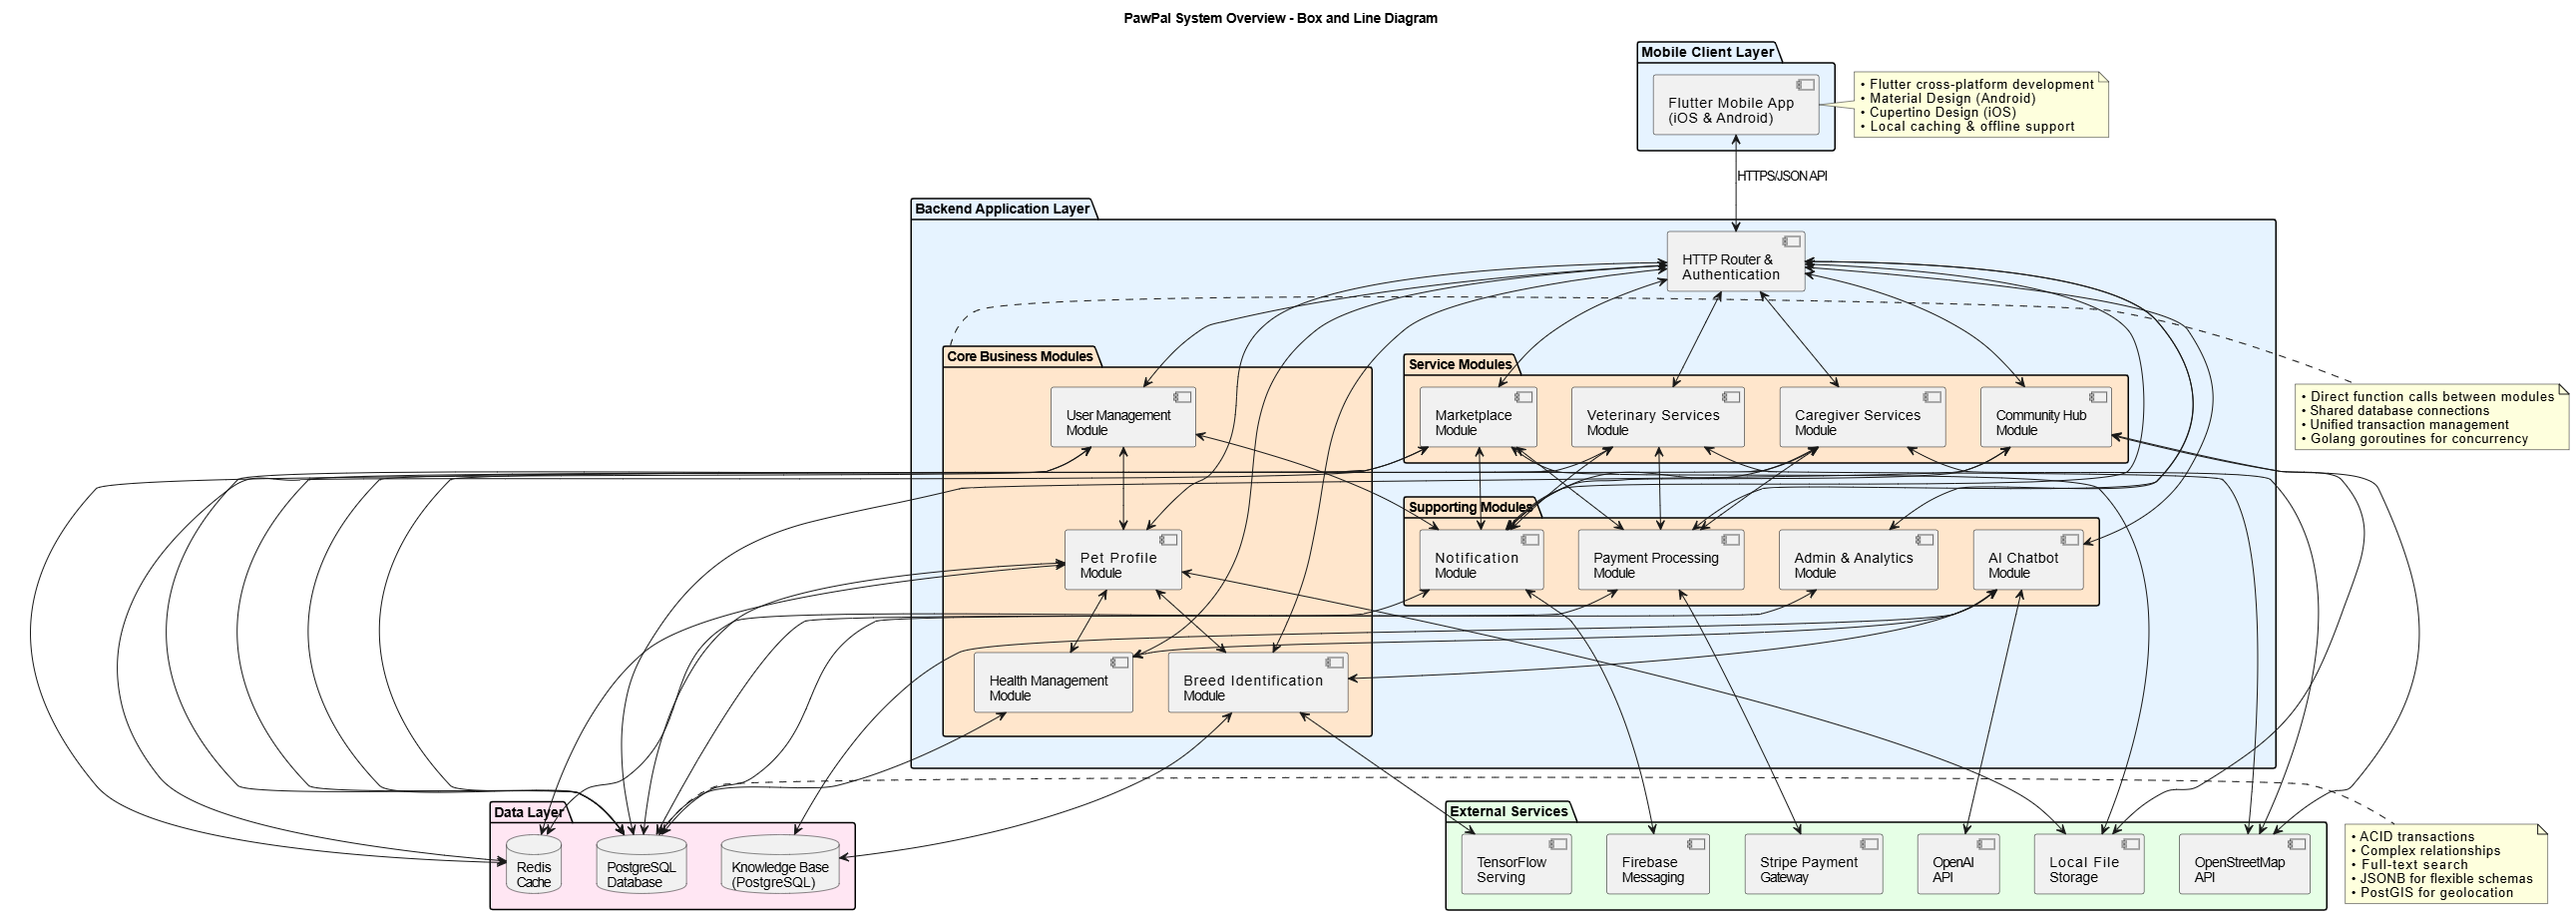
\includegraphics[width=1.0\textwidth]{ThesisFigs/system_overview_box_line.png}
    \caption{PawPal System Overview - Box and Line Diagram}
    \label{fig:system_overview}
\end{figure}

The diagram shows the mobile client layer communicating with the backend API gateway, which routes requests to the appropriate business modules. The backend modules interact with the data layer (PostgreSQL, Redis) and integrate with external services for payments, mapping, storage, and AI/ML capabilities.

\subsection{Detailed Layered Architecture}

The system implements a five-tier layered architecture with clear separation of concerns:

\begin{figure}[htbp]
    \centering
    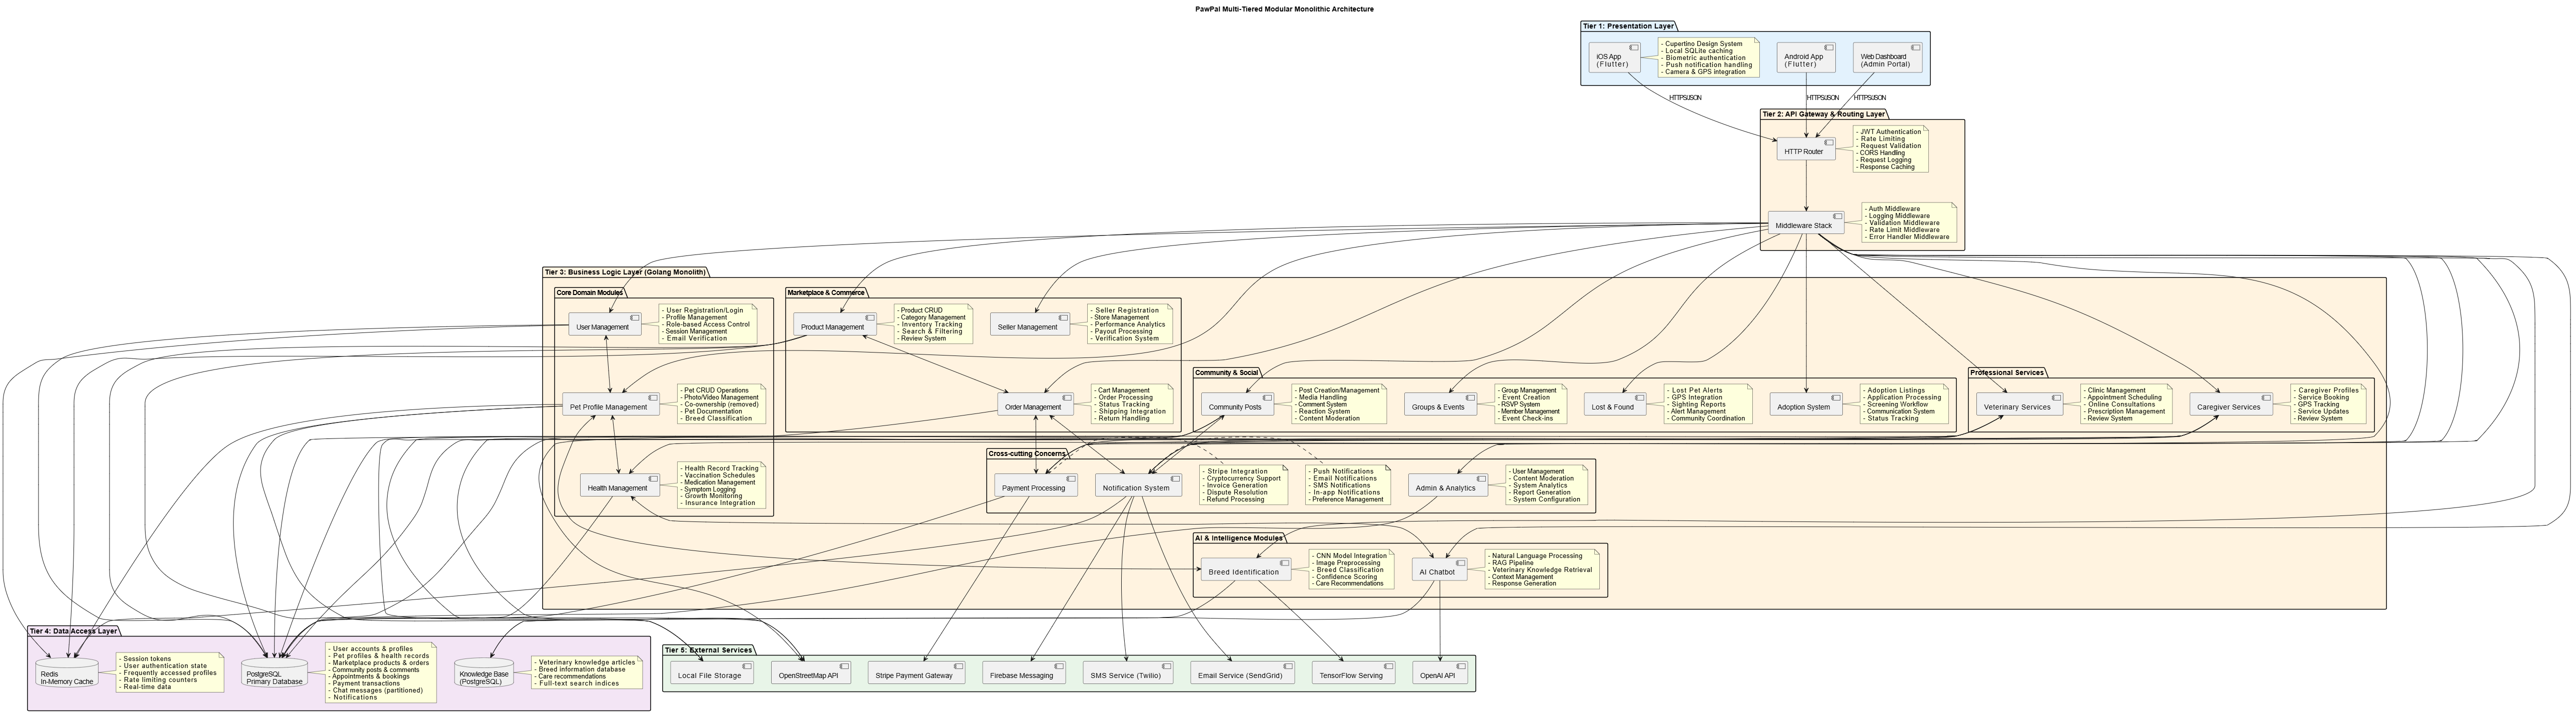
\includegraphics[width=1.0 \textwidth]{ThesisFigs/layered_architecture.png}
    \caption{PawPal Detailed Layered Architecture}
    \label{fig:layered_architecture}
\end{figure}

\textbf{Tier 1: Presentation Layer (Mobile Client)}
\begin{itemize}
    \item Flutter-based mobile applications for iOS and Android
    \item Handles user interface rendering and user interaction

    \item Communicates with backend via HTTPS REST APIs
    \item Manages client-side validation and state management
\end{itemize}

\textbf{Tier 2: API Gateway Layer}
\begin{itemize}
    \item Golang-based HTTP router serving as the request handler
    \item Routes incoming HTTP requests to appropriate internal modules
    \item Implements authentication and authorization middleware (JWT validation)
    \item Handles rate limiting and request throttling at the application level
    \item Provides centralized logging and request tracing
    \item Manages CORS policies and security headers
\end{itemize}

\textbf{Tier 3: Business Logic Layer (Internal Modules)}

The business logic is organized into eight core modules within the unified Golang application:

\begin{enumerate}
    \item \textbf{User Management Module:} User registration, login, JWT token management, password recovery, session handling, profile management
    \item \textbf{Pet Profile Module:} Pet CRUD operations, health records, vaccination tracking, journal entries, photo management
    \item \textbf{Health Management Module:} Health record management, vaccination schedules, medication tracking, reminder systems
    \item \textbf{Breed Identification Module:} Image processing, CNN model inference, breed information retrieval, care recommendations
    \item \textbf{Marketplace Module:} Product listings, search/filter, cart management, order processing, inventory tracking
    \item \textbf{Community Hub Module:} Post creation, social interactions, group management, event coordination, lost/found alerts
    \item \textbf{Veterinary Services Module:} Clinic registration, appointment booking, scheduling, reminders, consultation management
    \item \textbf{Caregiver Services Module:} Caregiver profiles, service matching, booking management, GPS tracking, service completion
\end{enumerate}

Supporting modules integrated across the core business logic:
\begin{itemize}
    \item \textbf{Payment Processing:}Cryptocurrency support, wallet management
    \item \textbf{AI Chatbot:} Query processing, RAG pipeline execution, LLM response generation, conversation history
    \item \textbf{Notification System:} Push notifications, email alerts, SMS messaging, in-app notifications
    \item \textbf{Admin \& Analytics:} System monitoring, user analytics, business intelligence, reporting
\end{itemize}

\textbf{Tier 4: Data Access Layer}
\begin{itemize}
    \item PostgreSQL database for all transactional and persistent data with ACID guarantees
    \item Redis cache for session tokens, frequently accessed profiles, and real-time data
  
\end{itemize}

\textbf{Tier 5: External Services Layer}
\begin{itemize}
    \item OpenStreetMap API for geolocation services
    \item Local file system for media storage
    \item Firebase Cloud Messaging for push notifications
    \item OpenAI API or other for LLM capabilities
    \item TensorFlow Serving for CNN model inference
\end{itemize}

\subsection{Module Communication and Integration}

Within the modular monolithic architecture, modules communicate through well-defined internal interfaces and direct function calls rather than network-based APIs. This approach provides several key advantages:

\textbf{Direct Function Calls:} Modules invoke each other's exported functions directly within the same process space, eliminating network latency and serialization overhead. For example, when the Marketplace Module processes an order, it directly calls the Payment Module's \texttt{ProcessPayment()} function and the Notification Module's \texttt{SendOrderConfirmation()} function.

\textbf{Shared Resources:} All modules share database connection pools, Redis cache connections, and configuration management, reducing resource consumption and ensuring consistent state across the application.

\textbf{Transaction Management:} Database transactions can span multiple modules seamlessly. For instance, creating a veterinary appointment can update the appointment table, deduct payment, and log the transaction within a single ACID transaction, ensuring data consistency without complex distributed transaction protocols.

\textbf{Error Propagation:} Errors propagate through the call stack naturally, simplifying debugging and error handling compared to distributed systems where failures may occur across network boundaries.

\textbf{Asynchronous Processing:} For operations that don't require immediate responses (e.g., sending email notifications, generating reports), the application uses Golang's goroutines and channels for efficient background processing within the same application, without requiring external message queue infrastructure.

\subsection{Golang Backend Implementation}

The Golang backend leverages Go's strengths for PawPal's modular monolithic architecture:

\begin{itemize}
    \item \textbf{Concurrency:} Goroutines handle multiple concurrent user requests efficiently within the single application, particularly important for real-time GPS tracking, payment processing, and chat functionality
    \item \textbf{Performance:} Single compiled binary with efficient memory management ensures sub-second response times for database queries and direct module function calls
    \item \textbf{Type Safety:} Static typing reduces runtime errors in critical payment and authentication logic, with compile-time verification of all module interfaces
    \item \textbf{Standard Library:} Built-in HTTP server, JSON parsing, and cryptography libraries simplify development within a single cohesive application

\end{itemize}



\section{Design Models}

PawPal follows an \textbf{Object-Oriented Development Approach} with well-defined classes, inheritance, and polymorphism in both Flutter frontend and Golang backend (using struct composition). The following UML diagrams model the system's static and dynamic behavior.

\subsection{Use Case Diagrams}

The use case diagrams provide a comprehensive view of the system's functional requirements and actor interactions across all modules.

\subsubsection{System-Wide Use Case Overview}

\begin{figure}[H]
    \centering
    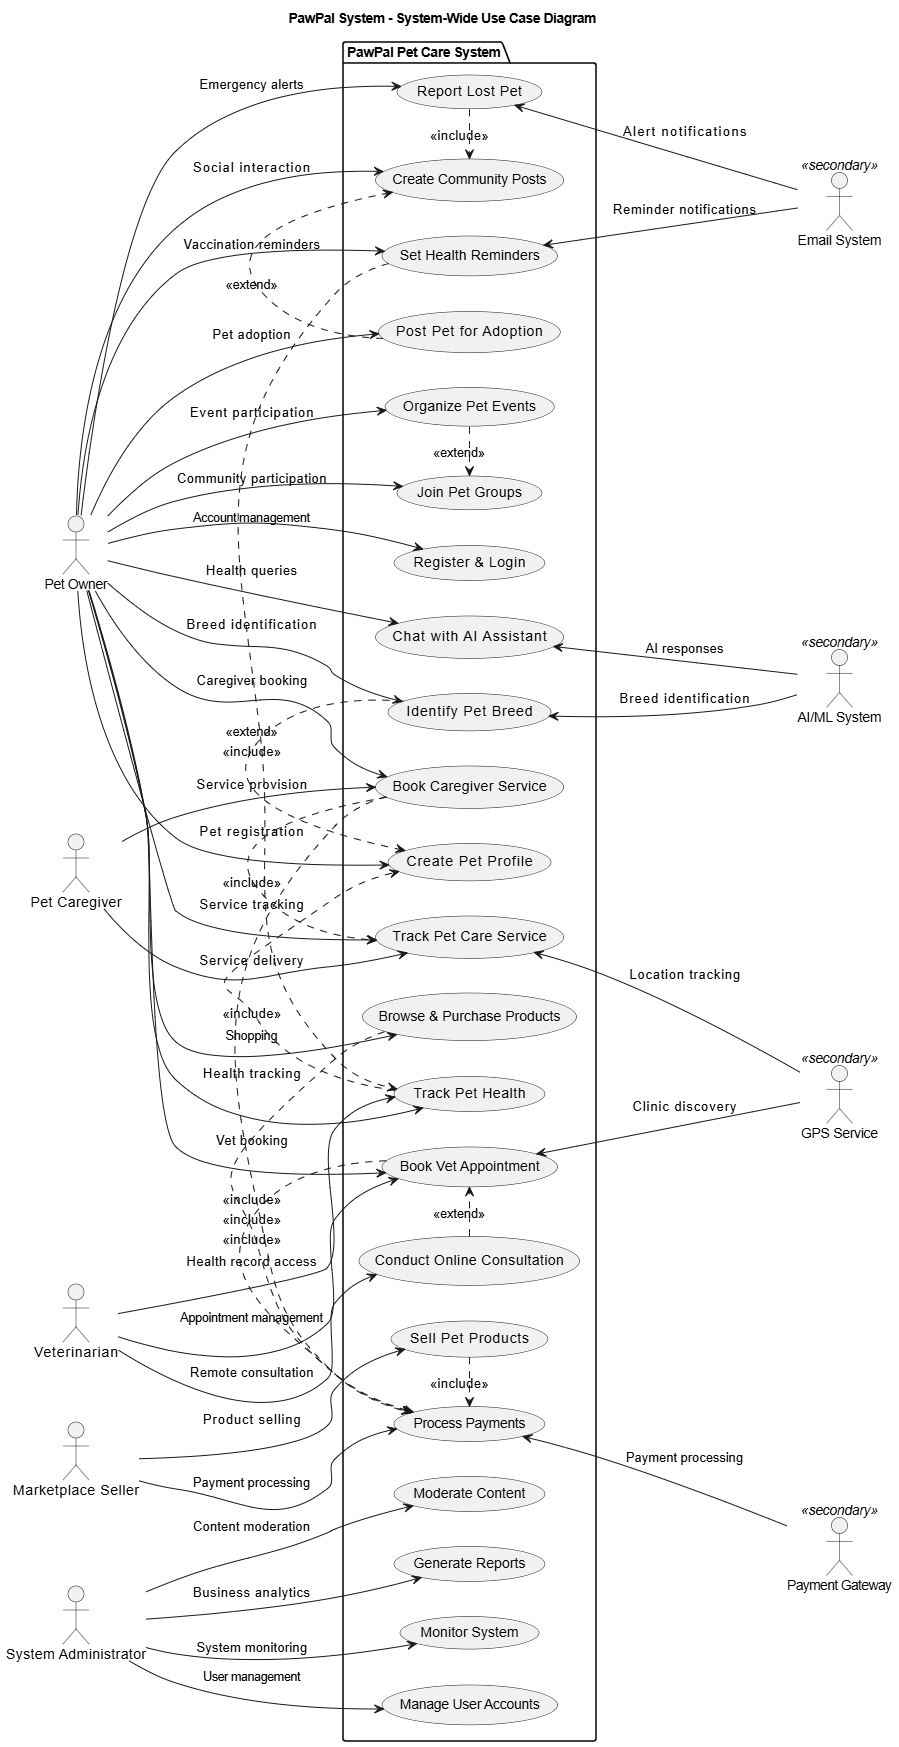
\includegraphics[width=0.75\textwidth]{ThesisFigs/use_case_system_wide.png}
    \caption{PawPal System-Wide Use Case Diagram}
    \label{fig:use_case_system_wide}
\end{figure}

This comprehensive use case diagram illustrates all system actors and their interactions with the core modules of PawPal. The diagram shows how Pet Owners, Veterinarians, Caregivers, Marketplace Sellers, and System Administrators interact with different functional areas of the system. The diagram includes 23 essential use cases organized by functional areas, with clear actor relationships and use case dependencies through include and extend relationships. 

\subsection{Component and Deployment Architecture}

\subsubsection{Component Architecture Diagram}

\begin{figure}[H]
    \centering
    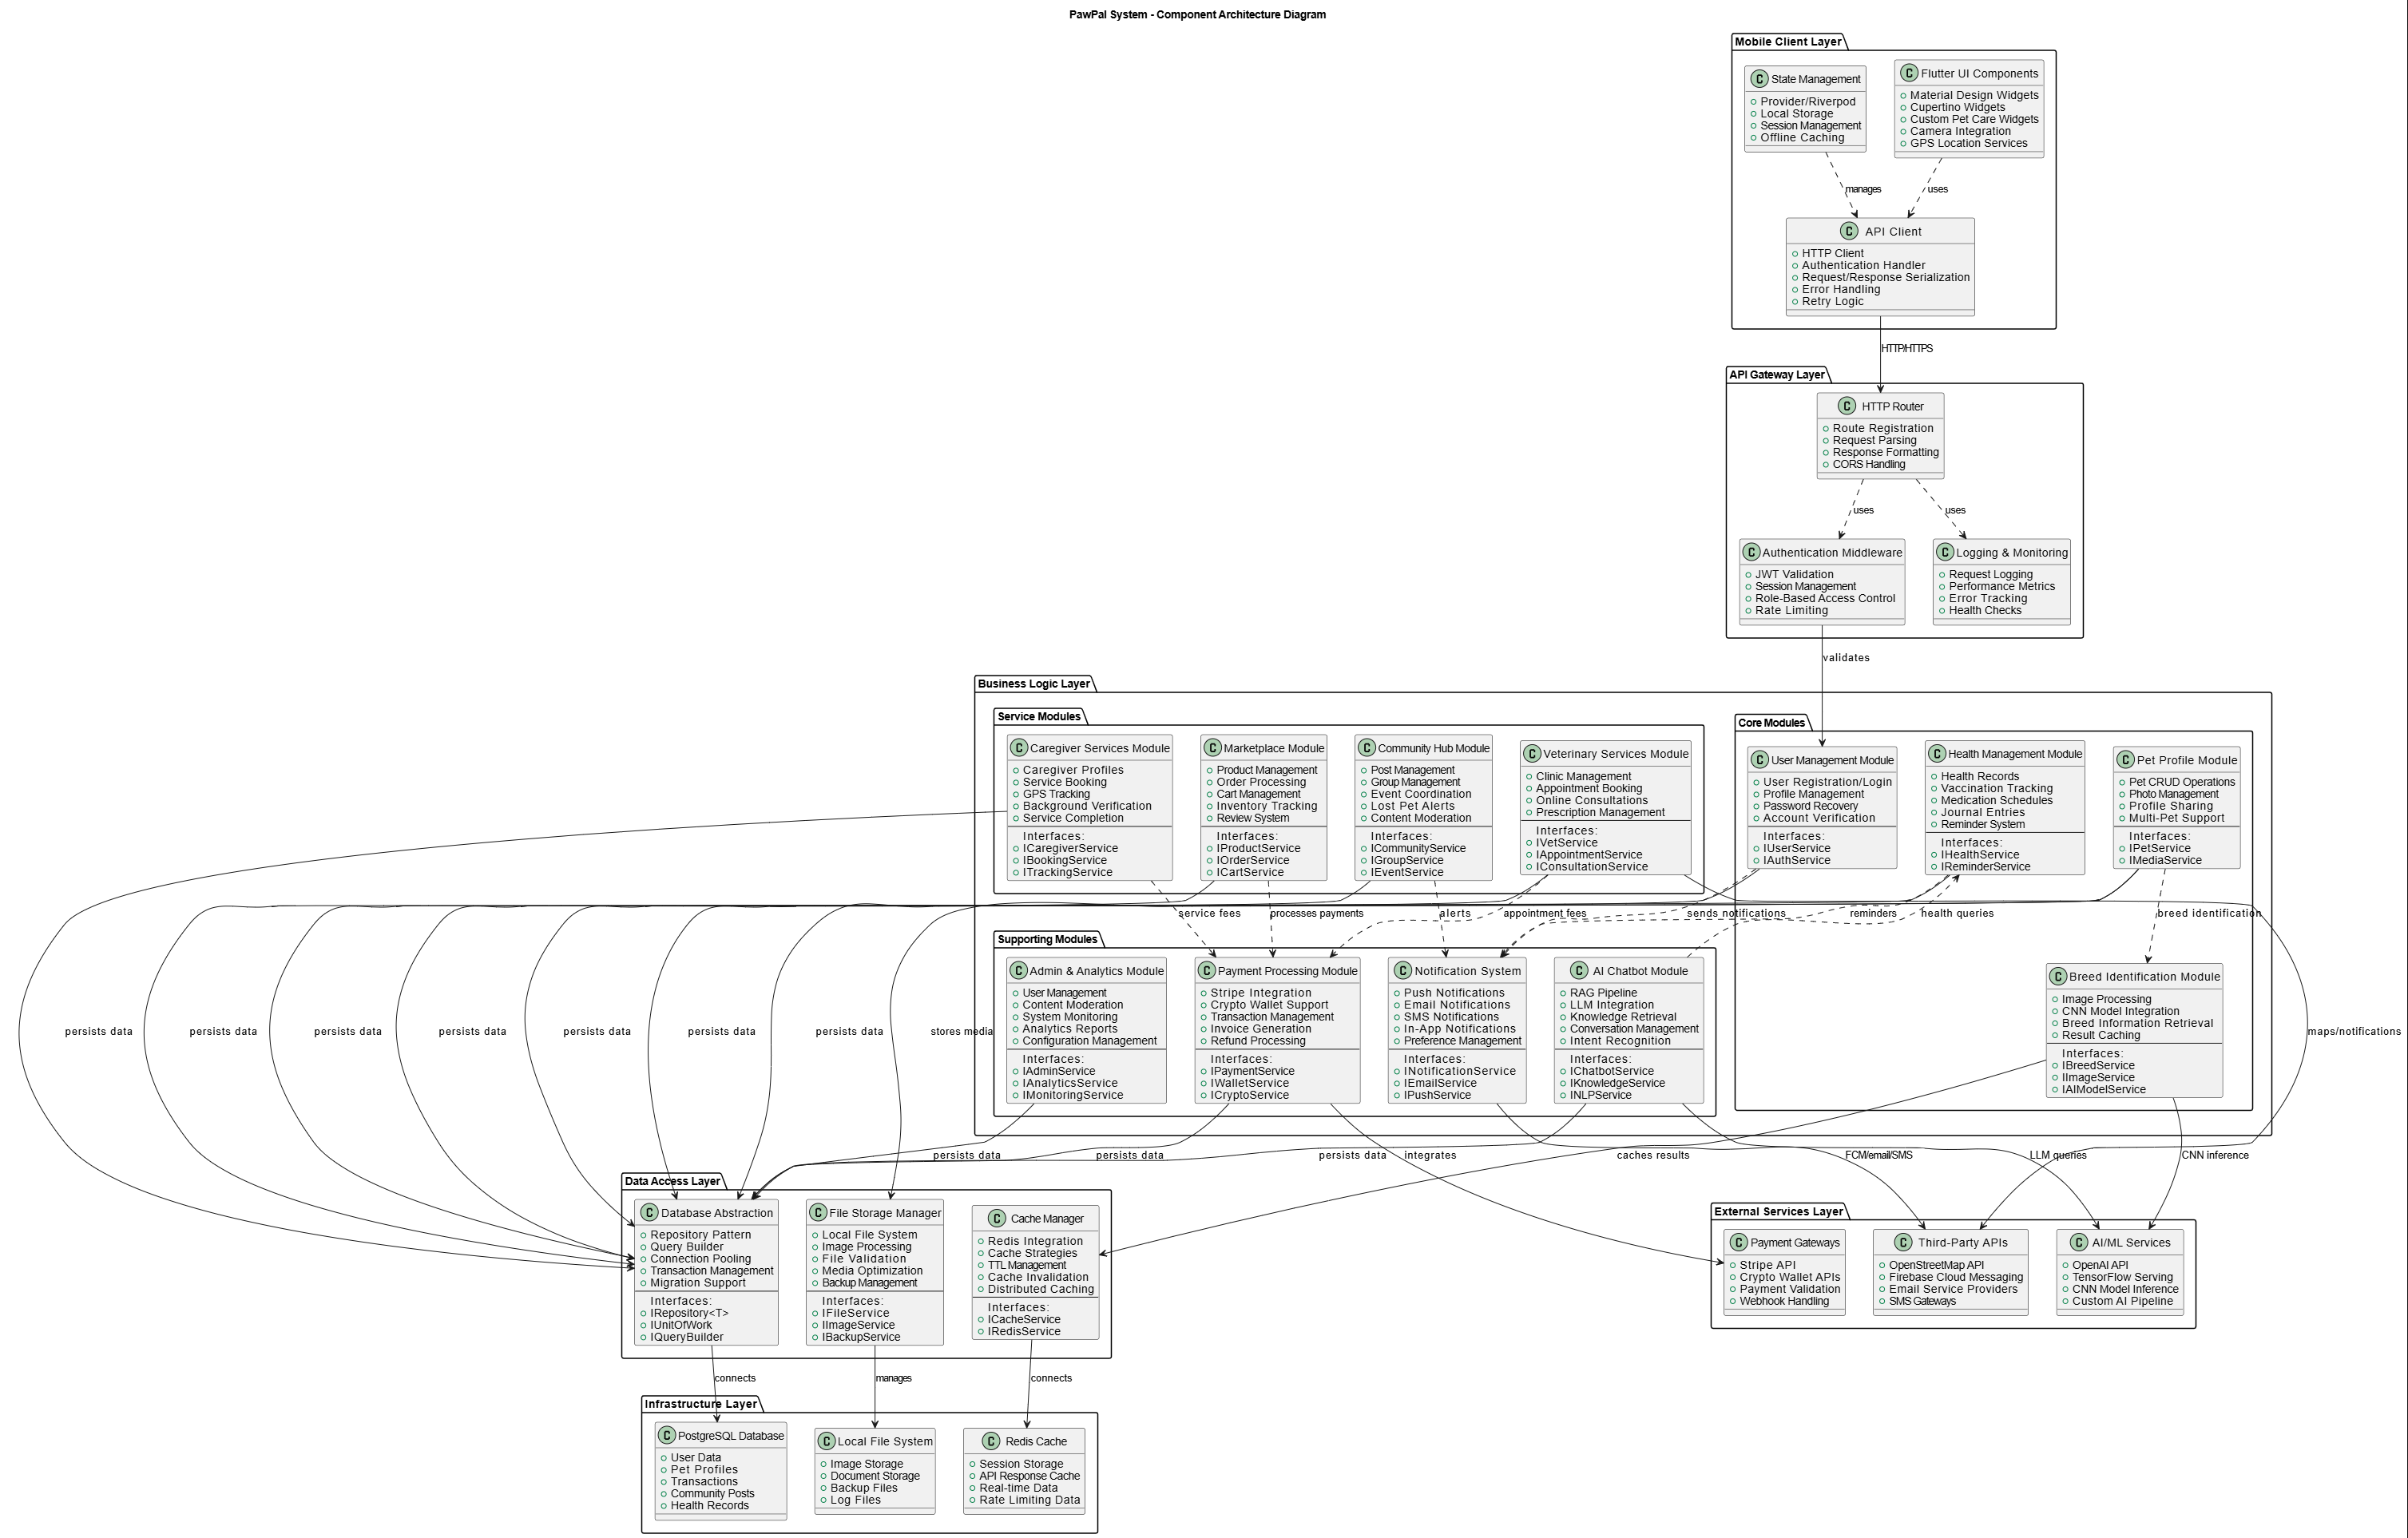
\includegraphics[width=1.0\textwidth]{ThesisFigs/component_architecture.png}
    \caption{PawPal Component Architecture Diagram}
    \label{fig:component_architecture}
\end{figure}

The component architecture diagram illustrates the internal structure of PawPal's modular monolithic backend, showing the relationships and dependencies between all system components. The diagram is organized into five distinct layers: Mobile Client Layer, API Gateway Layer, Business Logic Layer (with Core, Service, and Supporting modules), Data Access Layer, External Services Layer, and Infrastructure Layer. Each component includes its key responsibilities and interfaces, demonstrating the clear separation of concerns and well-defined module boundaries that enable maintainable and scalable architecture.

\subsubsection{Deployment Architecture Diagram}

\begin{figure}[H]
    \centering
    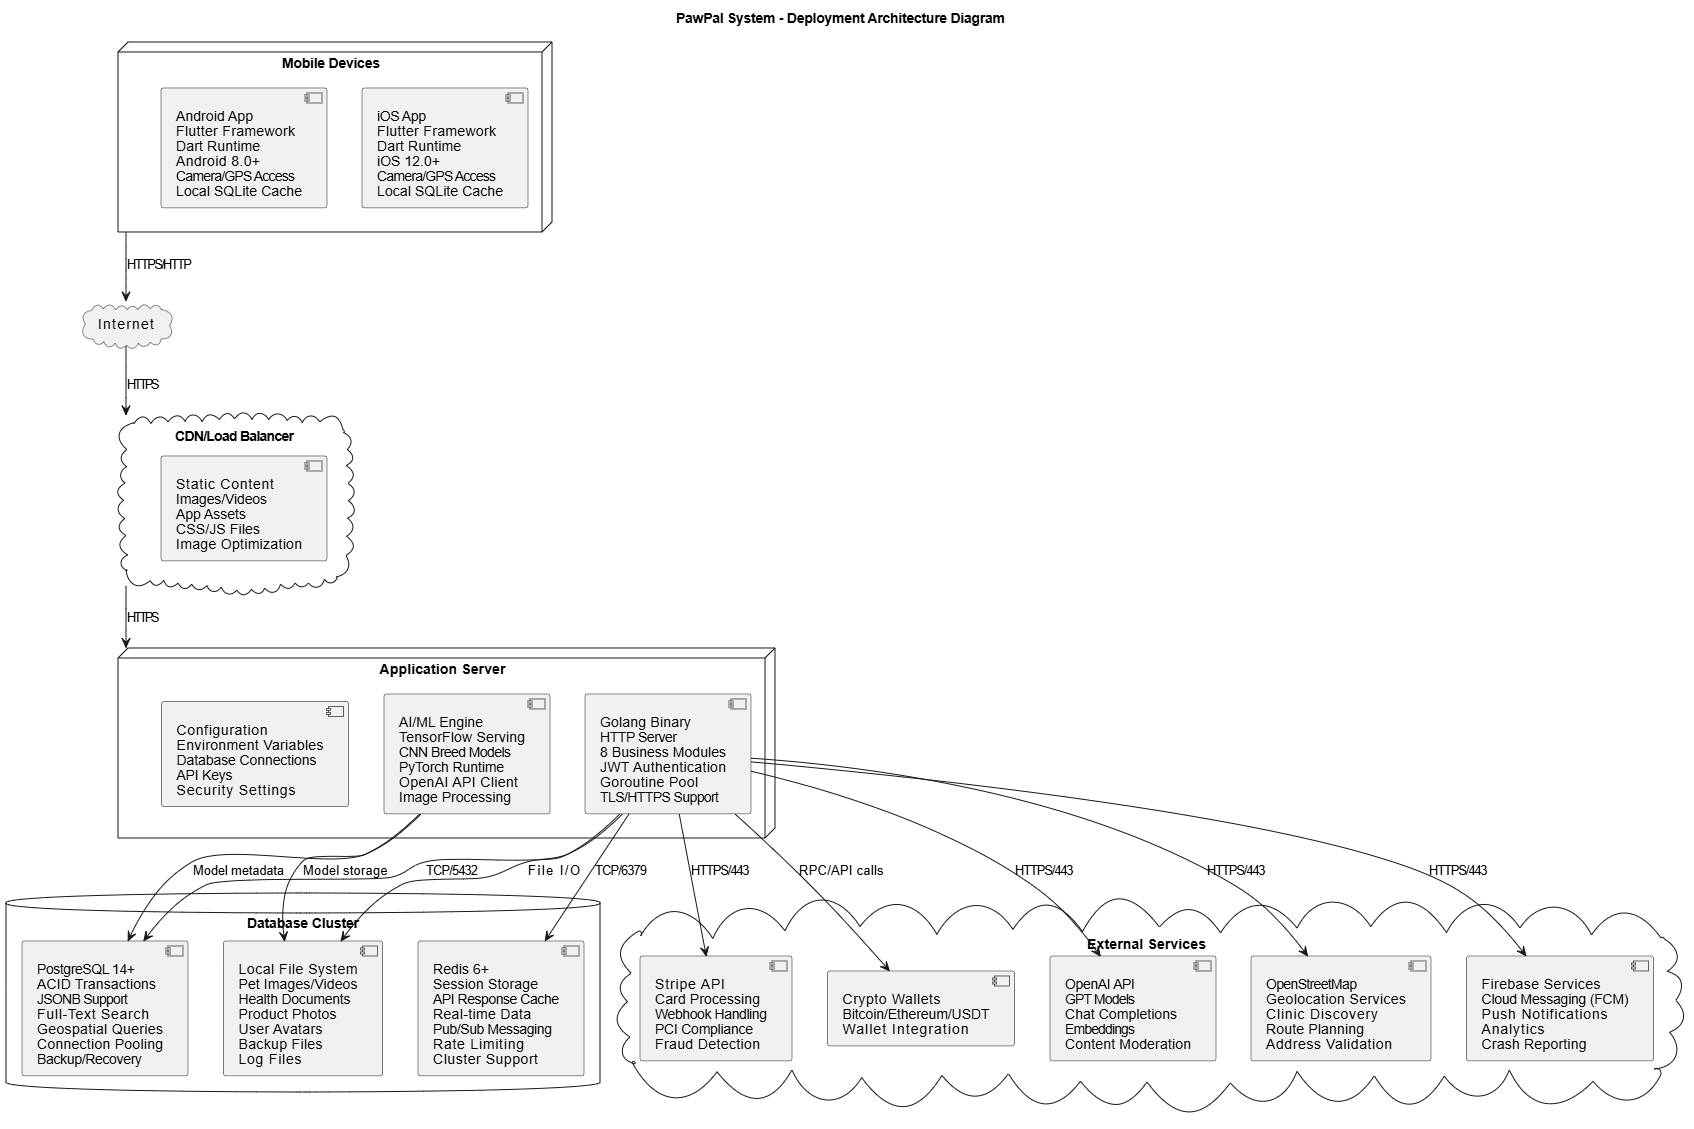
\includegraphics[width=1.0\textwidth]{ThesisFigs/deployment_architecture.png}
    \caption{PawPal Deployment Architecture Diagram}
    \label{fig:deployment_architecture}
\end{figure}

The deployment architecture diagram presents the physical deployment structure of PawPal, including mobile devices, application servers, database clusters, external services, and monitoring infrastructure. The diagram specifies the complete technology stack, hardware requirements, network protocols, security implementations, and deployment patterns. It shows how the Flutter mobile applications communicate with the Golang backend through HTTPS, the backend's integration with PostgreSQL and Redis, and the comprehensive monitoring and security infrastructure.

\subsection{Activity Diagrams}

\subsubsection{User Registration and Pet Profile Creation}

\begin{figure}[H]
    \centering
    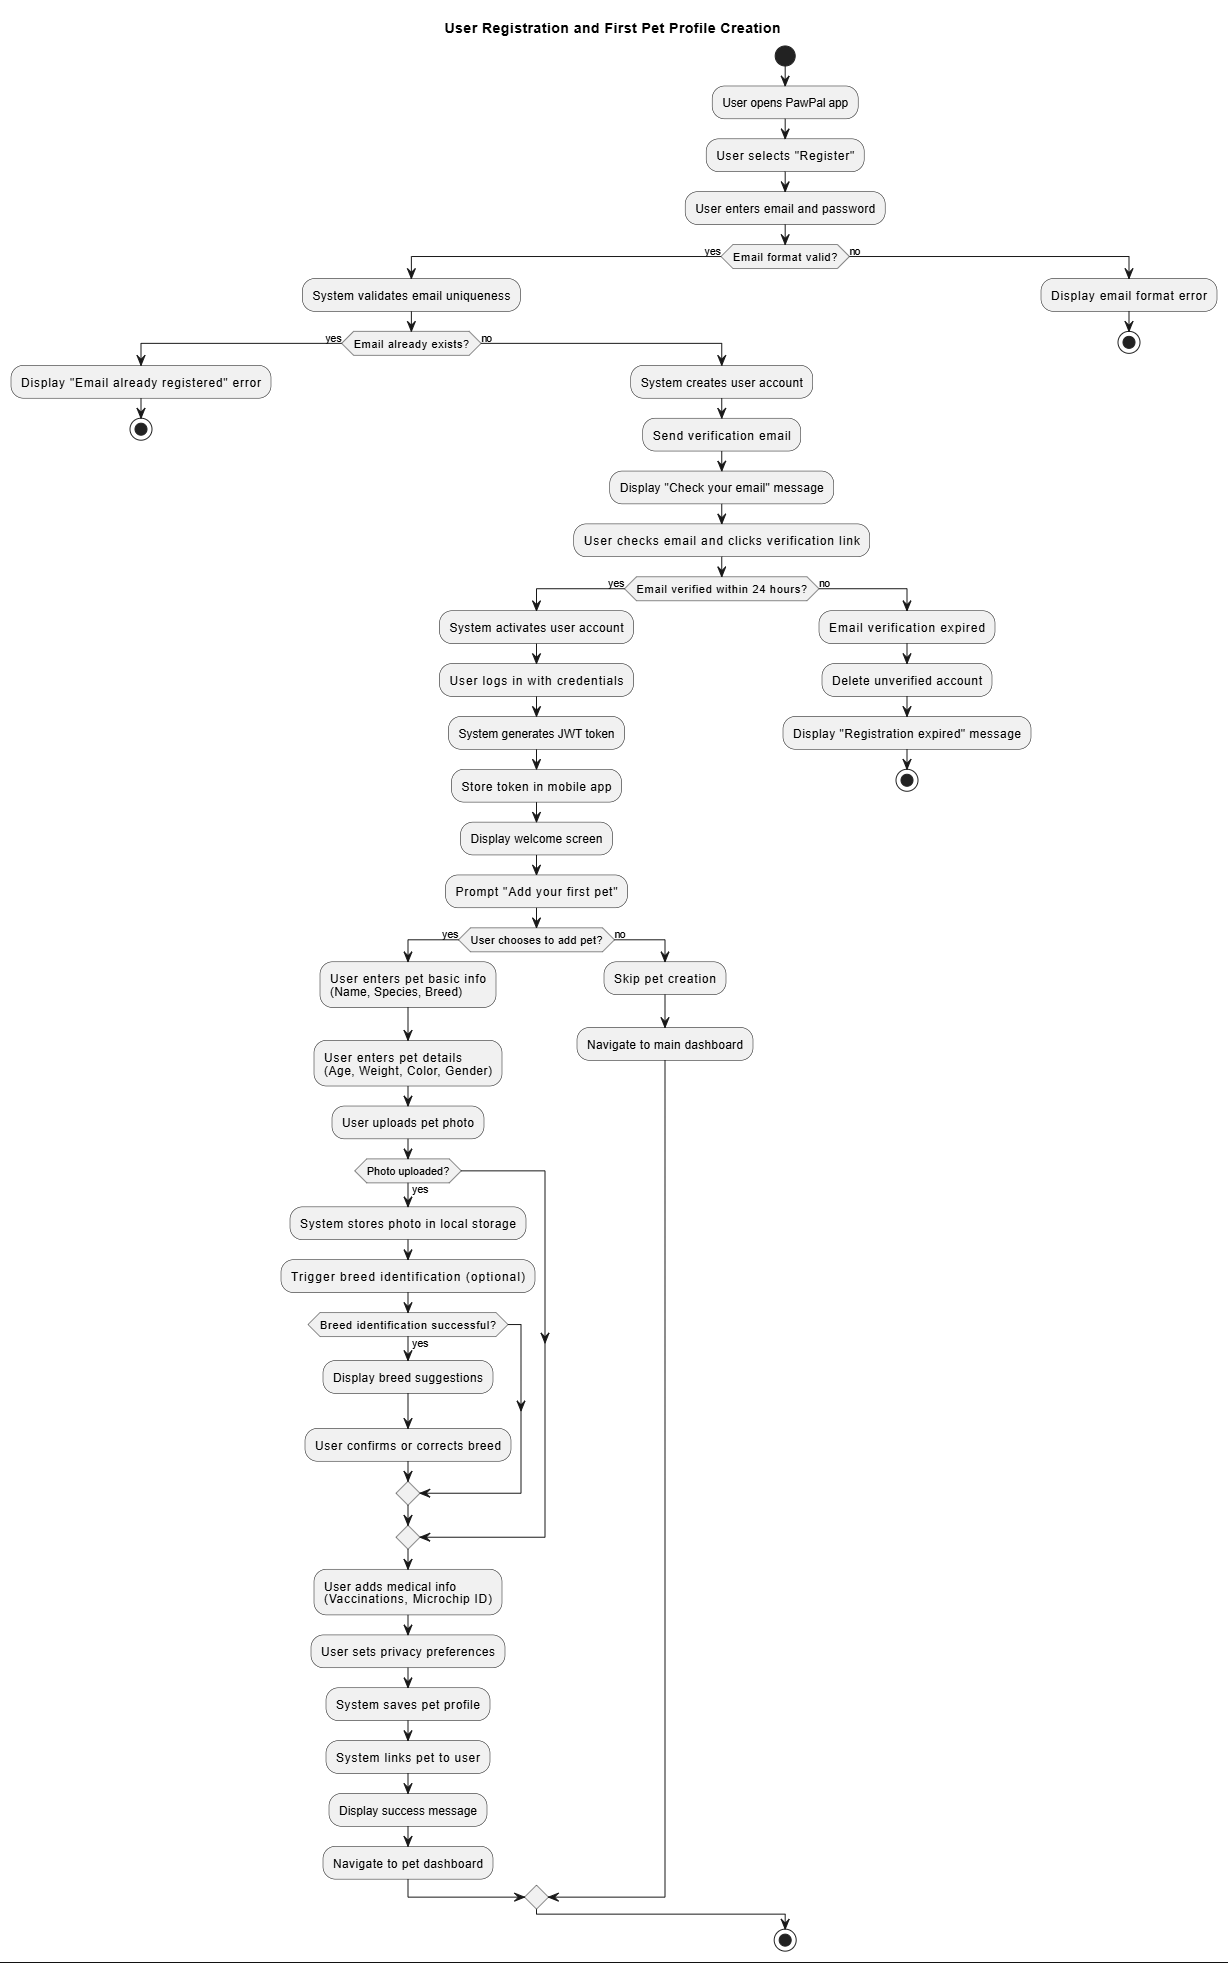
\includegraphics[width=0.9\textwidth]{ThesisFigs/activity_user_registration.png}
    \caption{User Registration and First Pet Profile Creation Activity Diagram}
    \label{fig:activity_user_registration}
\end{figure}

This activity diagram illustrates the registration workflow integrating authentication, email verification, and pet profile creation. The flow ensures data validation at each step and provides clear user feedback for validation failures and alternative flows.

% \subsubsection{Marketplace Purchase Flow}

% \begin{figure}[H]
%     \centering
%     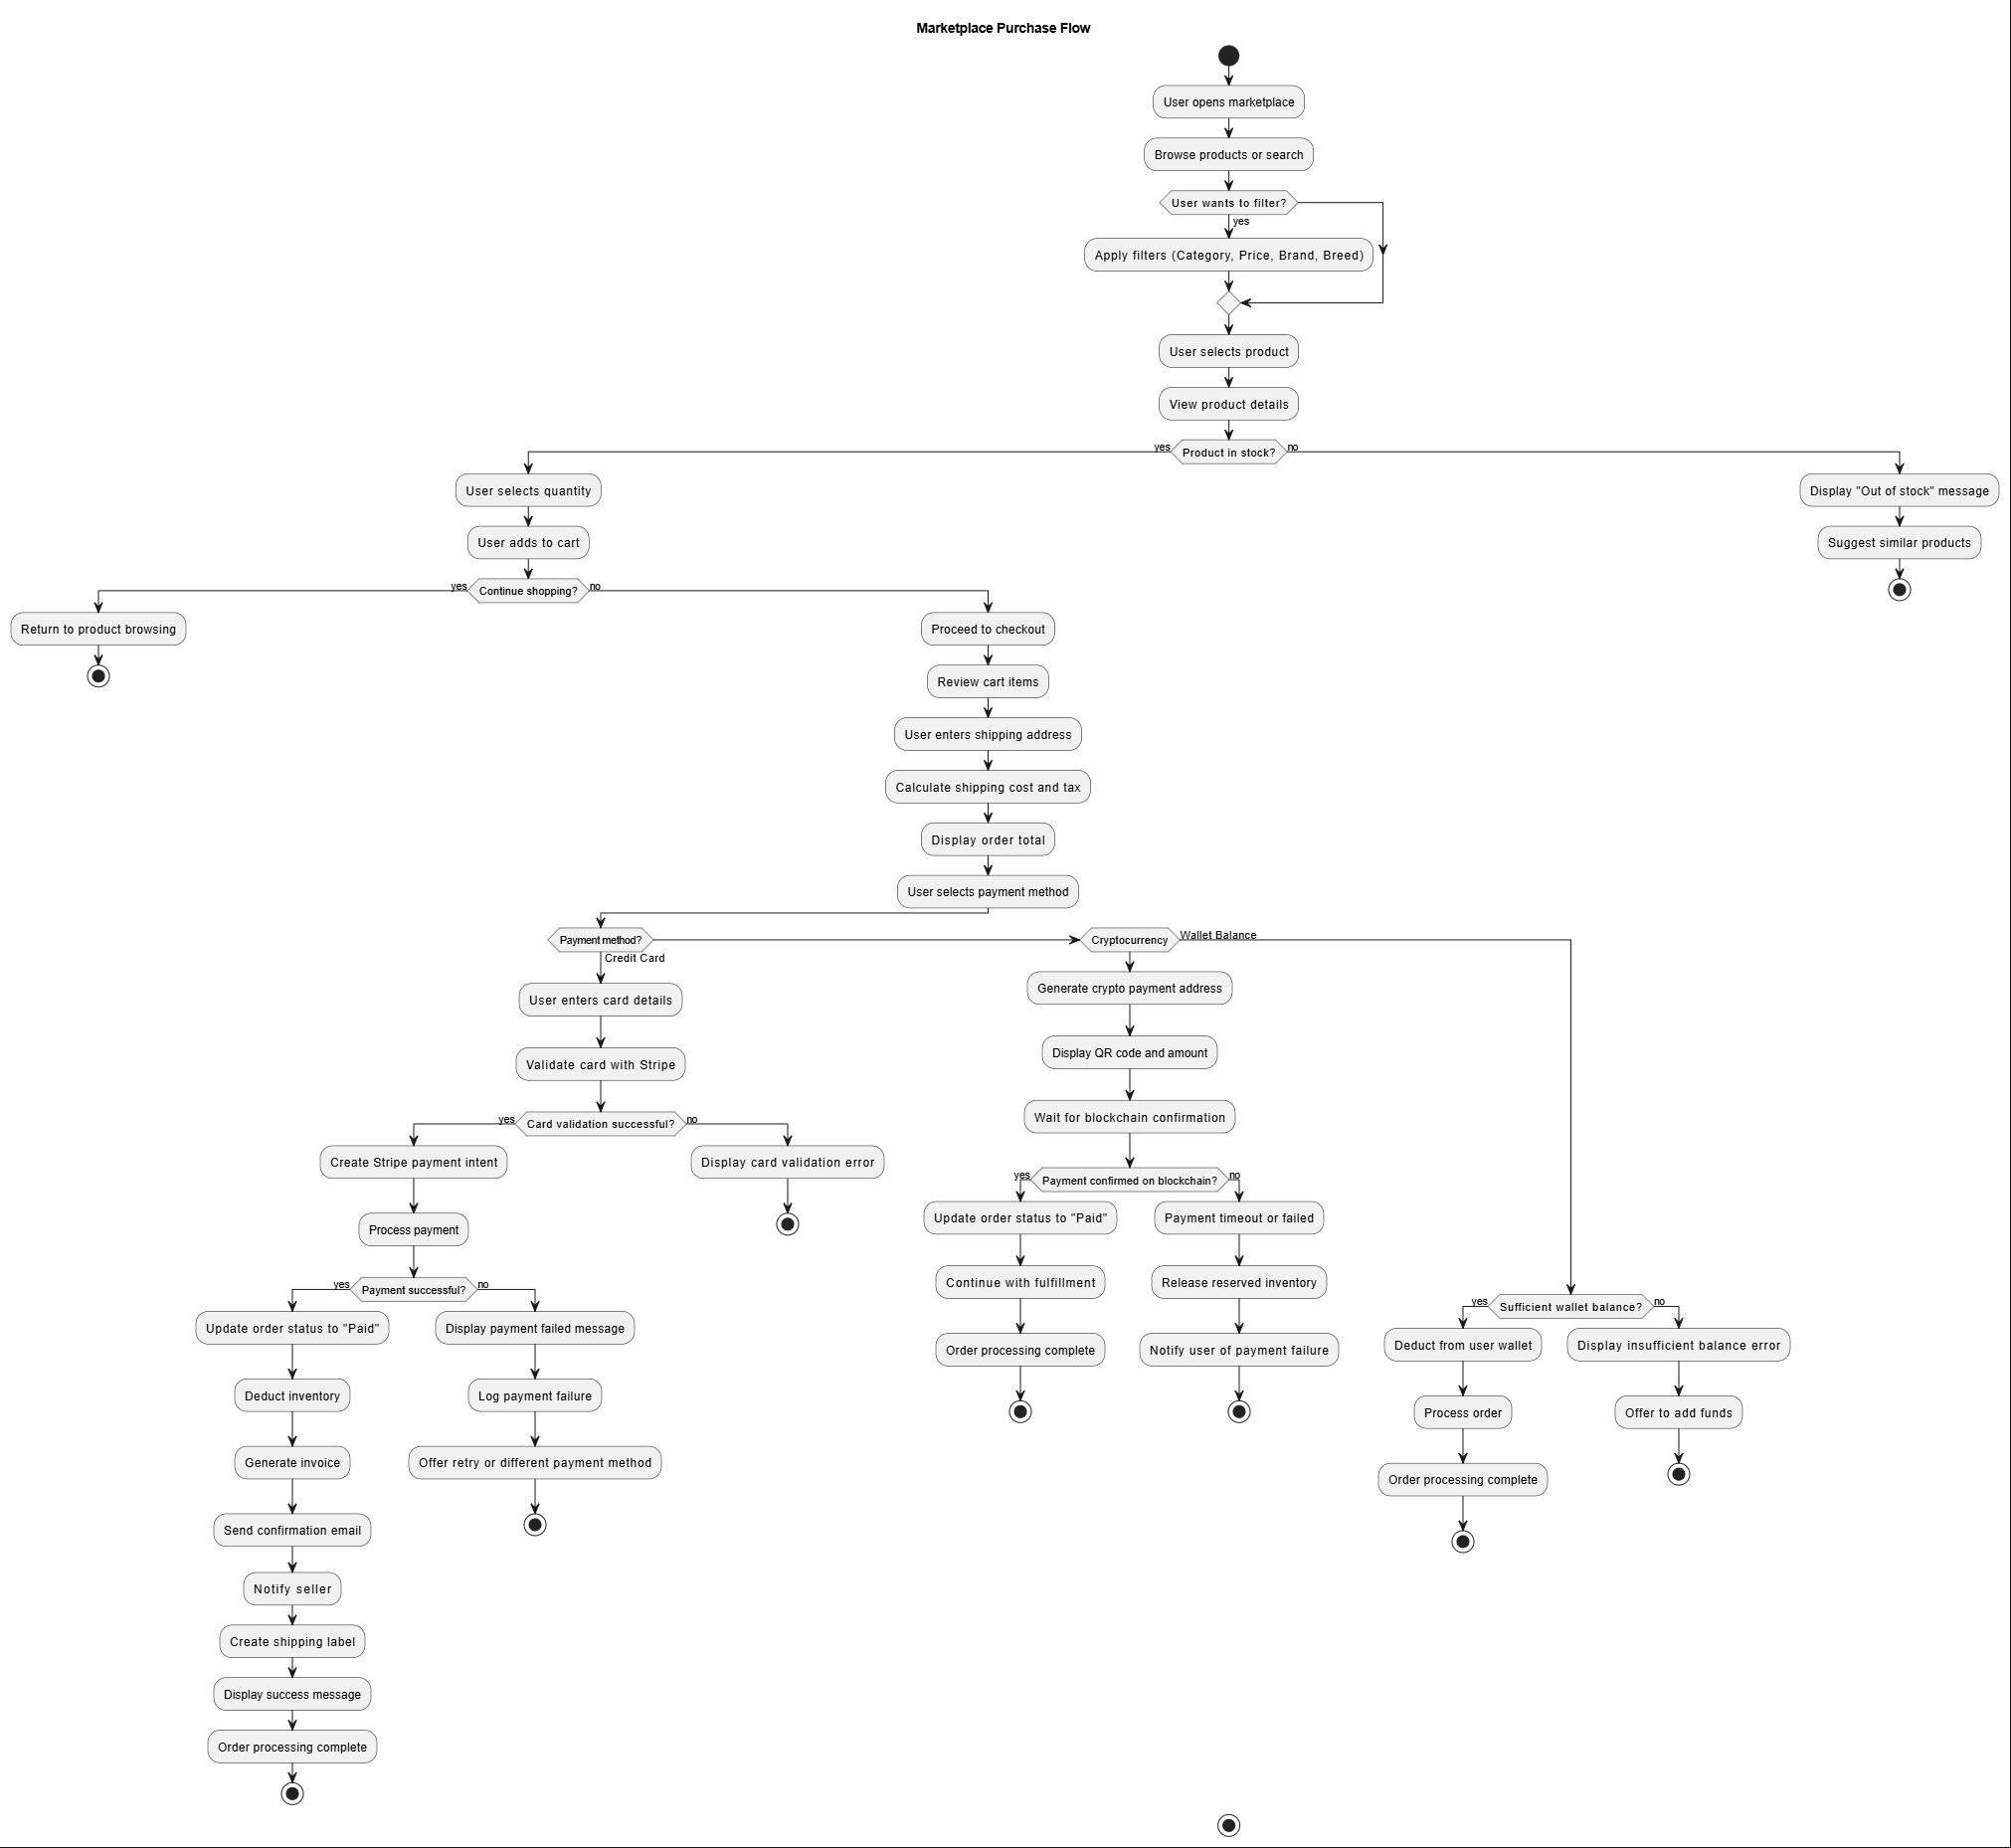
\includegraphics[width=0.9\textwidth]{ThesisFigs/activity_marketplace_purchase.png}
%     \caption{Marketplace Purchase Flow Activity Diagram}
%     \label{fig:activity_marketplace_purchase}
% \end{figure}

% This diagram models the complete e-commerce workflow including product discovery, cart management, payment processing with multiple gateways (card, crypto, wallet), and post-transaction notifications with error handling and retry mechanisms.

\subsubsection{Veterinary Appointment Booking}

\clearpage % Force new page for large diagram
\begin{figure}[htbp]
    \centering
    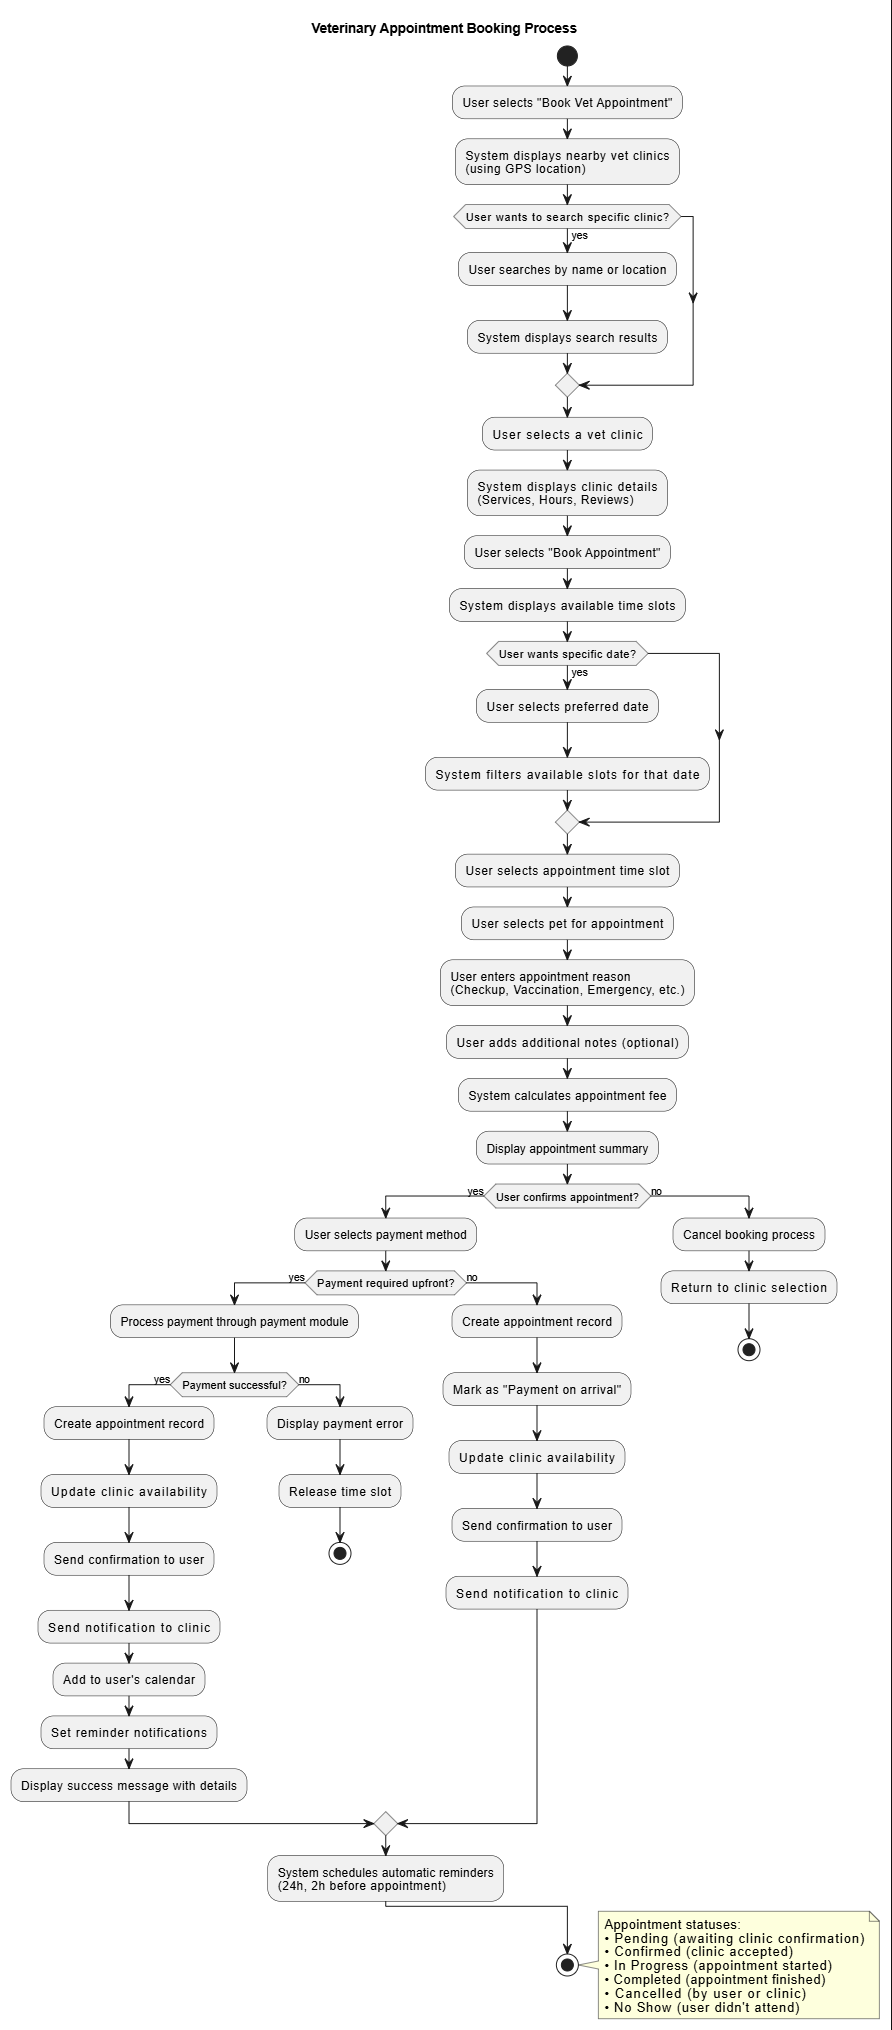
\includegraphics[width=0.75\textwidth]{ThesisFigs/activity_vet_appointment.png}
    \caption{Veterinary Appointment Booking Activity Diagram}
    \label{fig:activity_vet_appointment}
\end{figure}

This activity diagram shows the appointment booking process including clinic discovery using GPS, availability checking, booking confirmation, and payment processing with reminder scheduling.

\subsubsection{AI Breed Identification Process}

\begin{figure}[H]
    \centering
    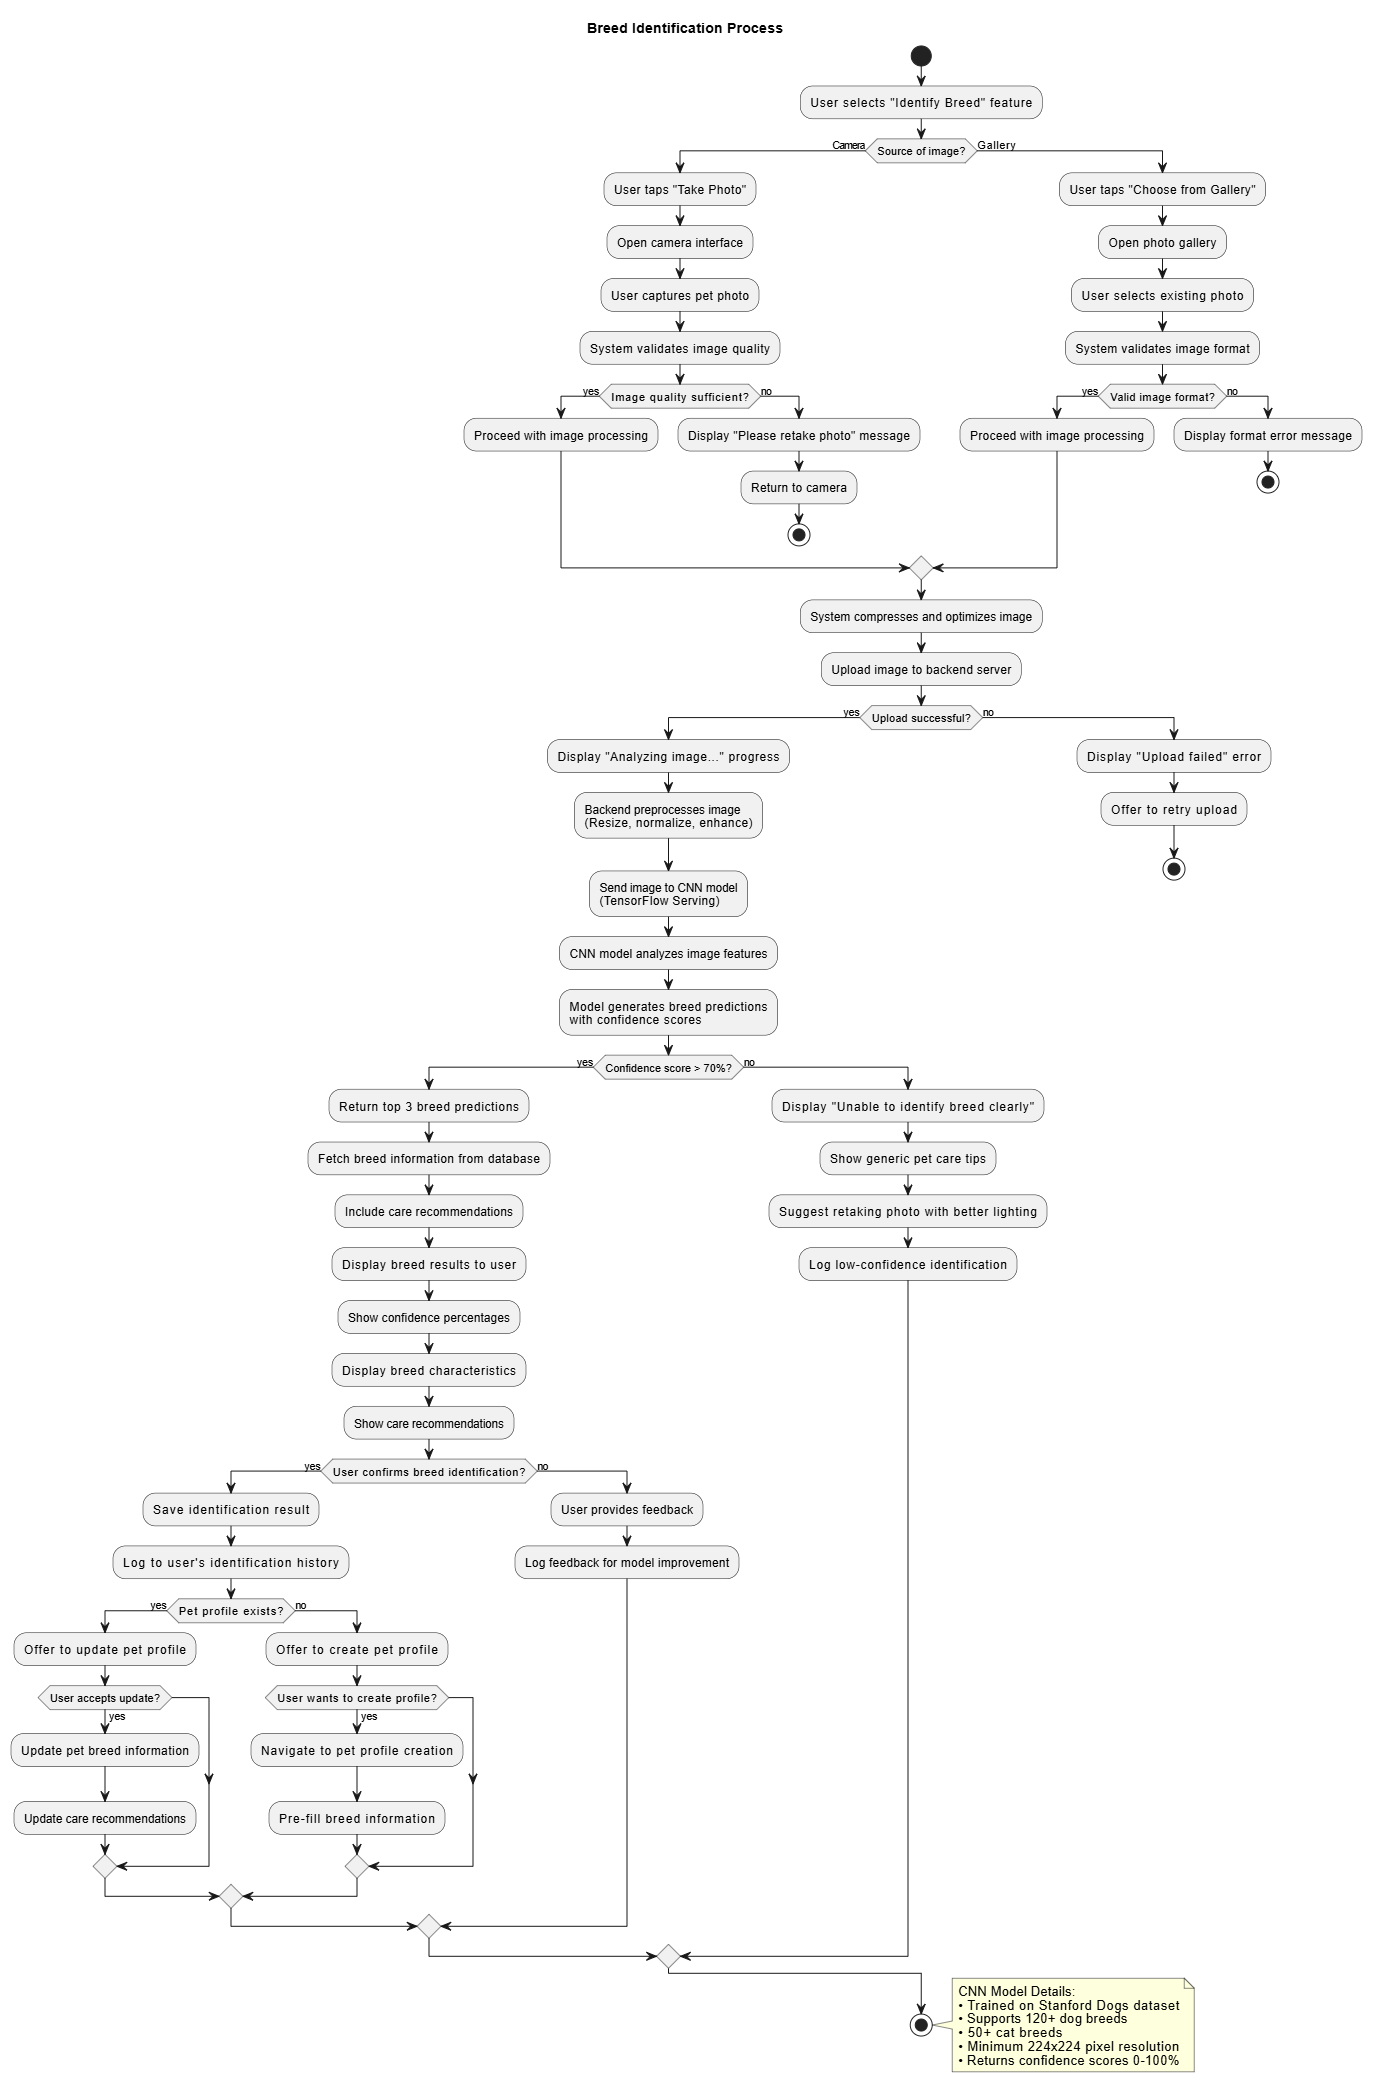
\includegraphics[width=0.9\textwidth]{ThesisFigs/activity_breed_identification.png}
    \caption{AI Breed Identification Process Activity Diagram}
    \label{fig:activity_breed_identification}
\end{figure}

This diagram illustrates the AI-powered breed identification workflow including image upload, validation, CNN model processing, confidence scoring, and result presentation with option to save to pet profile.

\subsubsection{Caregiver Service Booking Flow}

\begin{figure}[H]
    \centering
    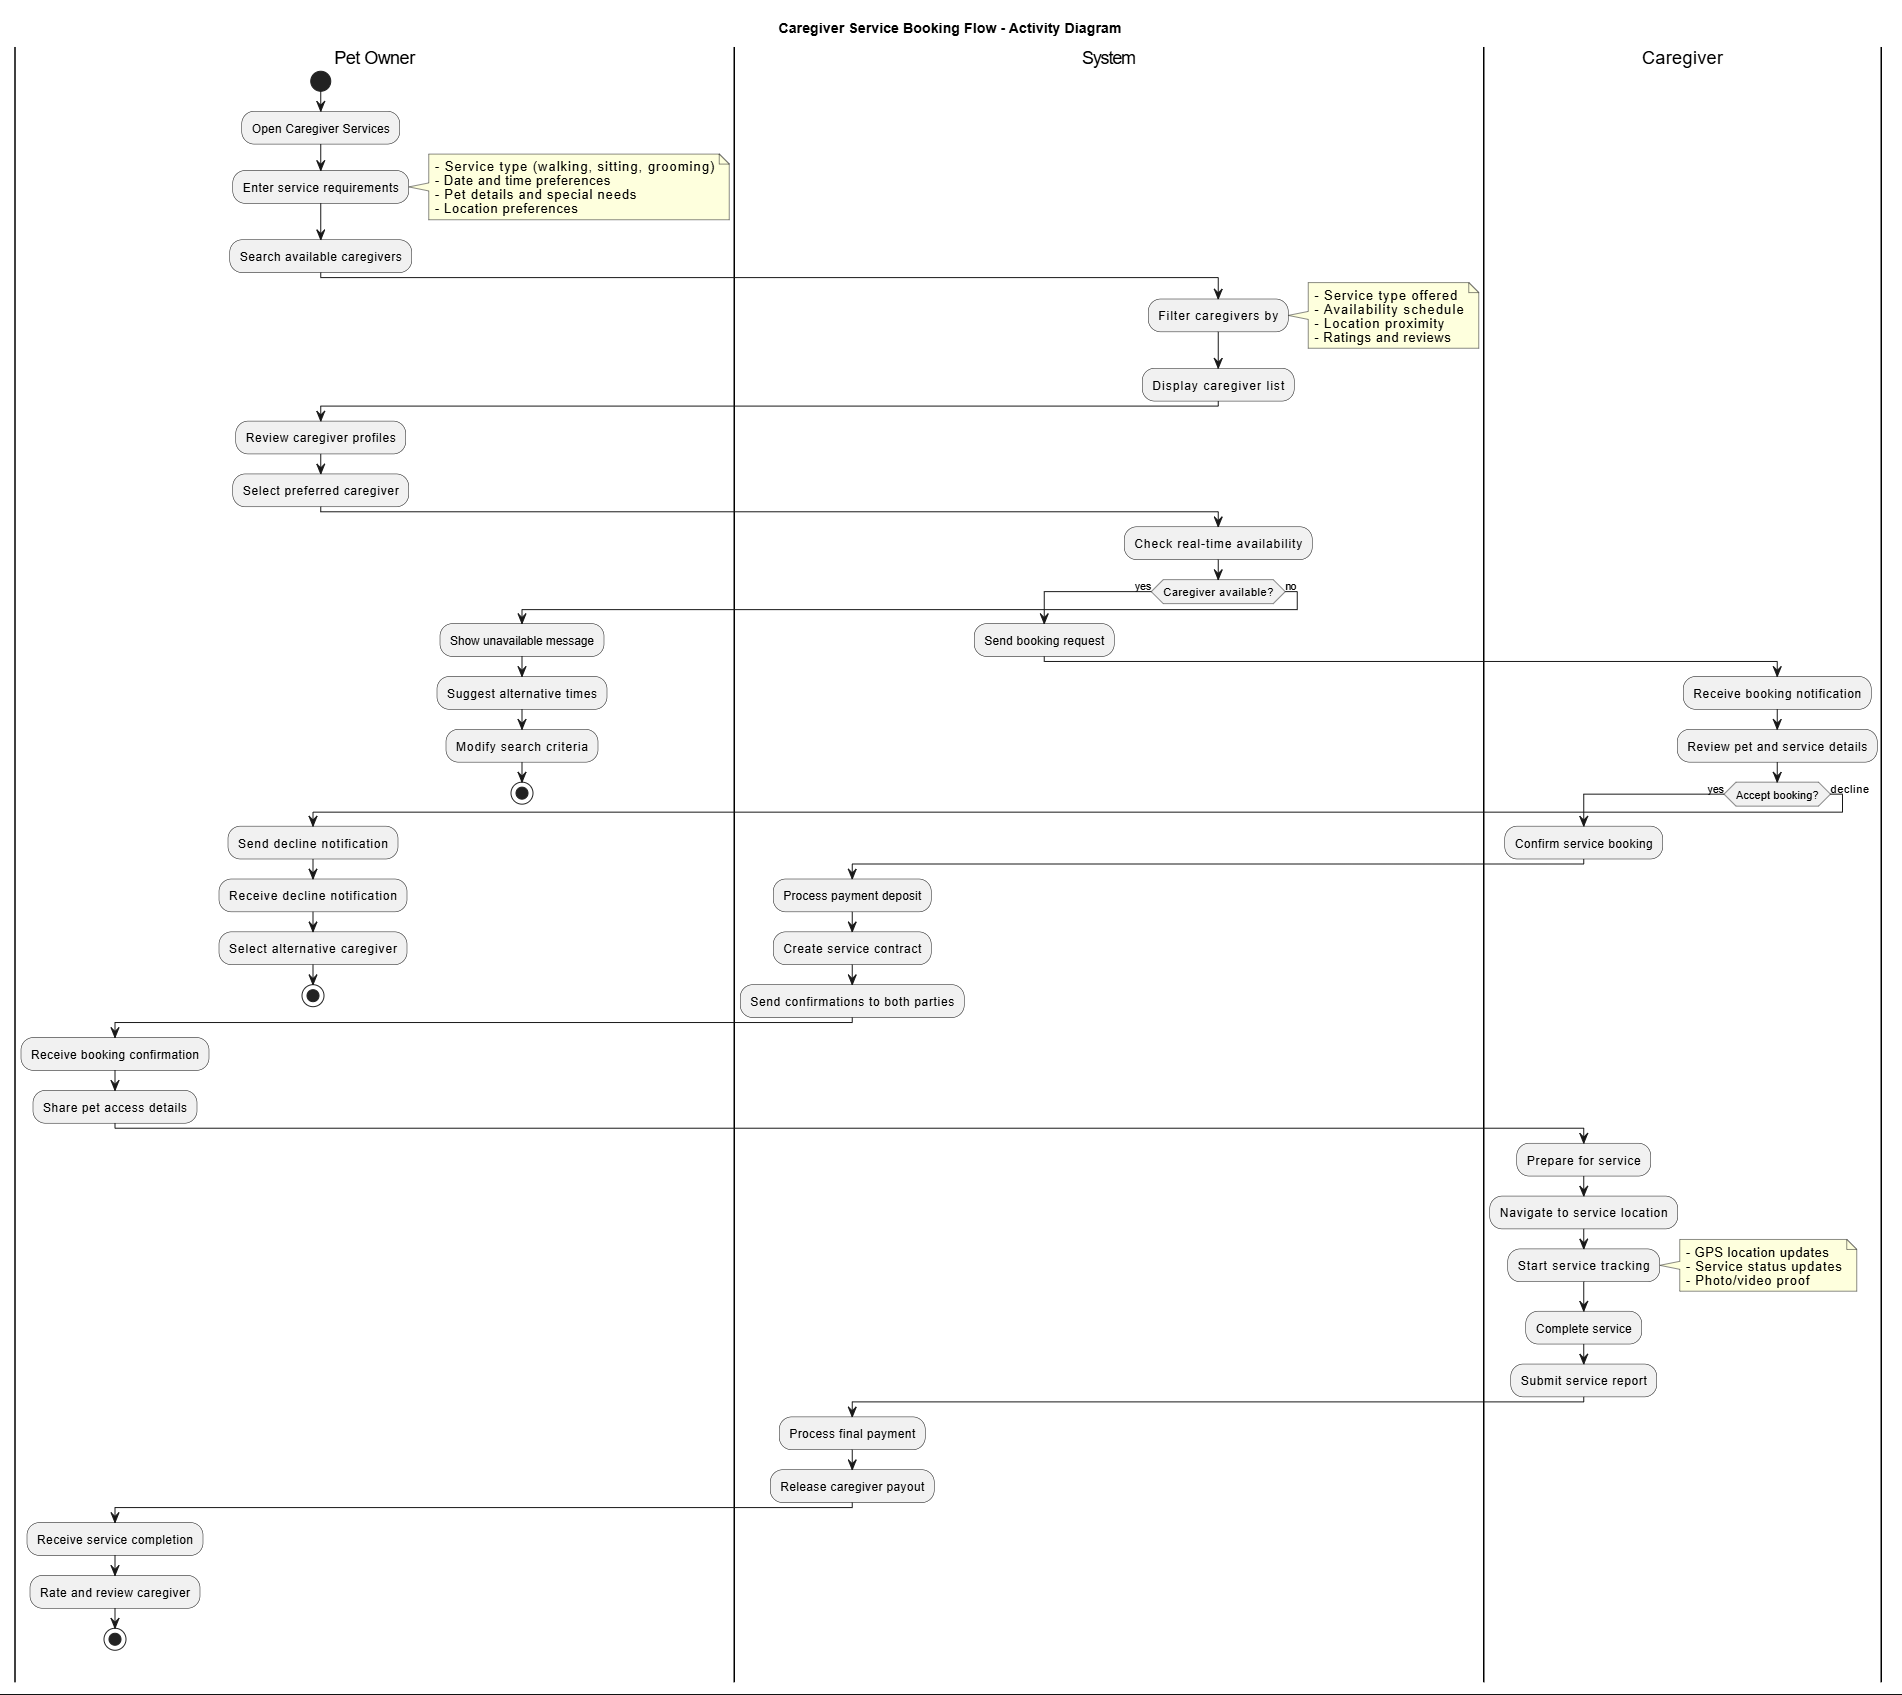
\includegraphics[width=0.9\textwidth]{ThesisFigs/activity_caregiver_booking.png}
    \caption{Caregiver Service Booking Activity Diagram}
    \label{fig:activity_caregiver_booking}
\end{figure}

This activity diagram models the complete caregiver service booking workflow with swim lanes for Pet Owner, System, and Caregiver actors. The flow includes service request submission, caregiver matching based on location and availability, real-time GPS tracking during service delivery, photo updates with progress reports, and payment processing upon completion.

\subsubsection{AI Chatbot Conversation Flow}

\begin{figure}[H]
    \centering
    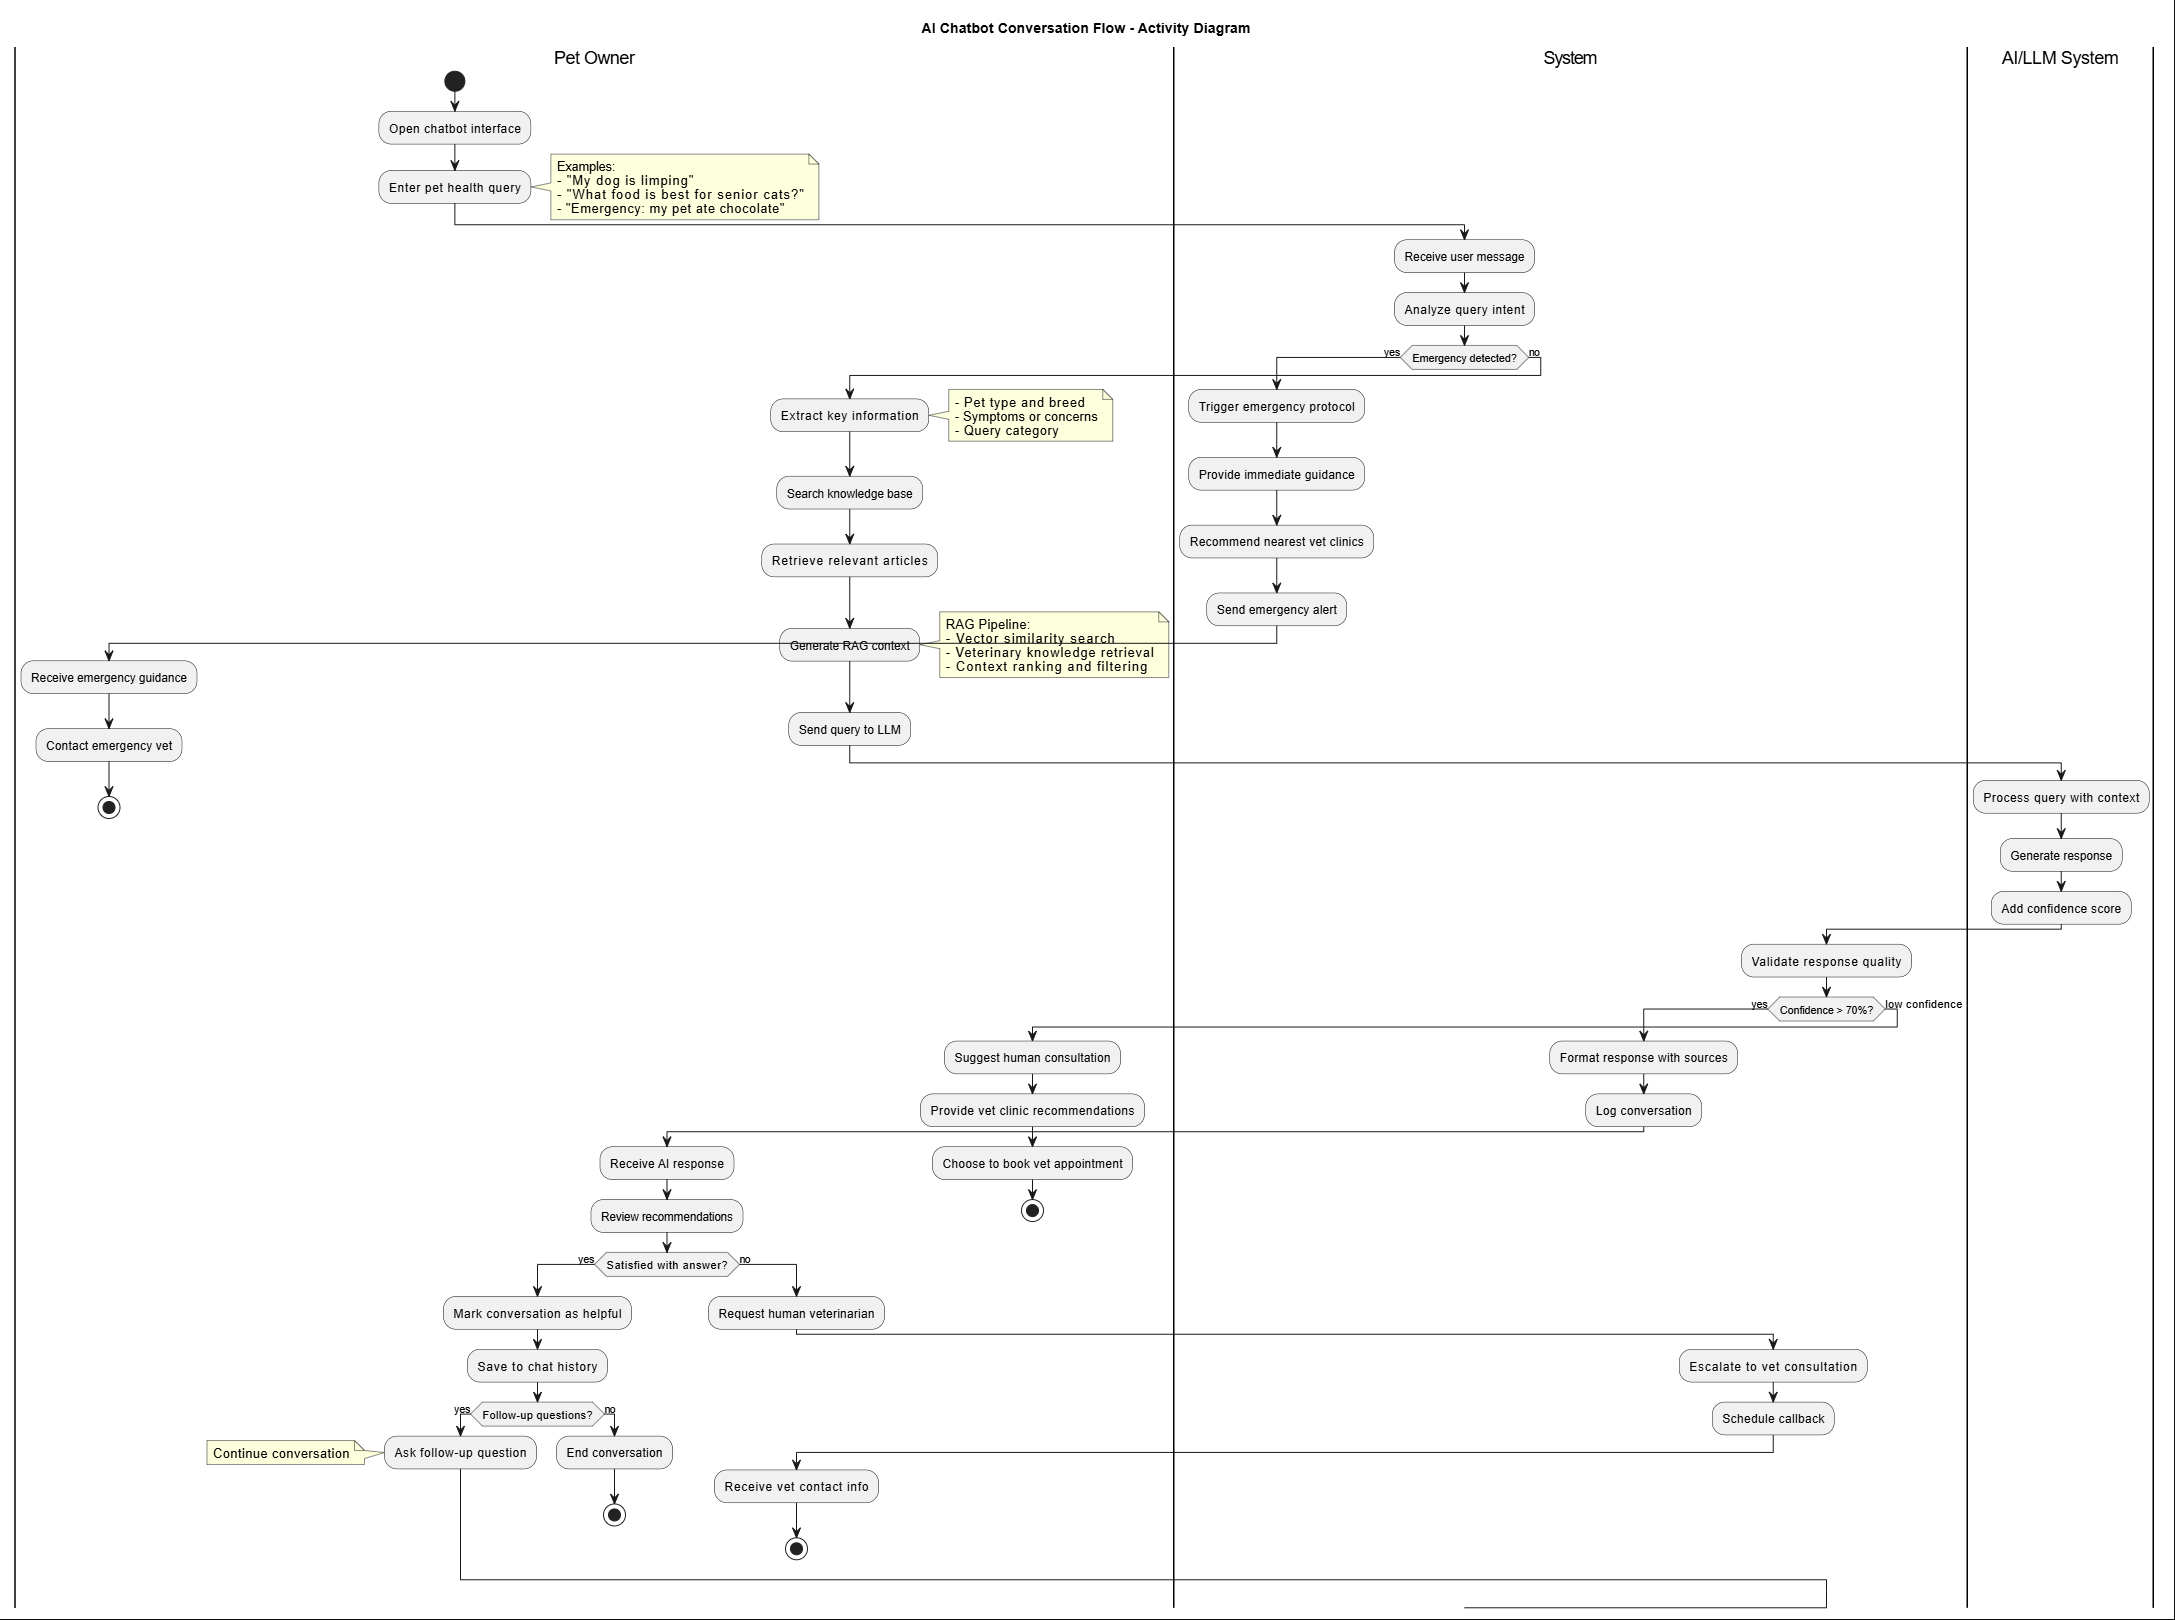
\includegraphics[width=0.9\textwidth]{ThesisFigs/activity_chatbot_conversation.png}
    \caption{AI Chatbot Conversation Activity Diagram}
    \label{fig:activity_chatbot_conversation}
\end{figure}

This diagram illustrates the AI-powered chatbot conversation flow including intent analysis, emergency detection, RAG knowledge retrieval, LLM processing, confidence scoring, and veterinarian escalation for critical situations. The workflow ensures appropriate responses based on query complexity and urgency levels.

\subsubsection{Lost Pet Alert System}

\begin{figure}[H]
    \centering
    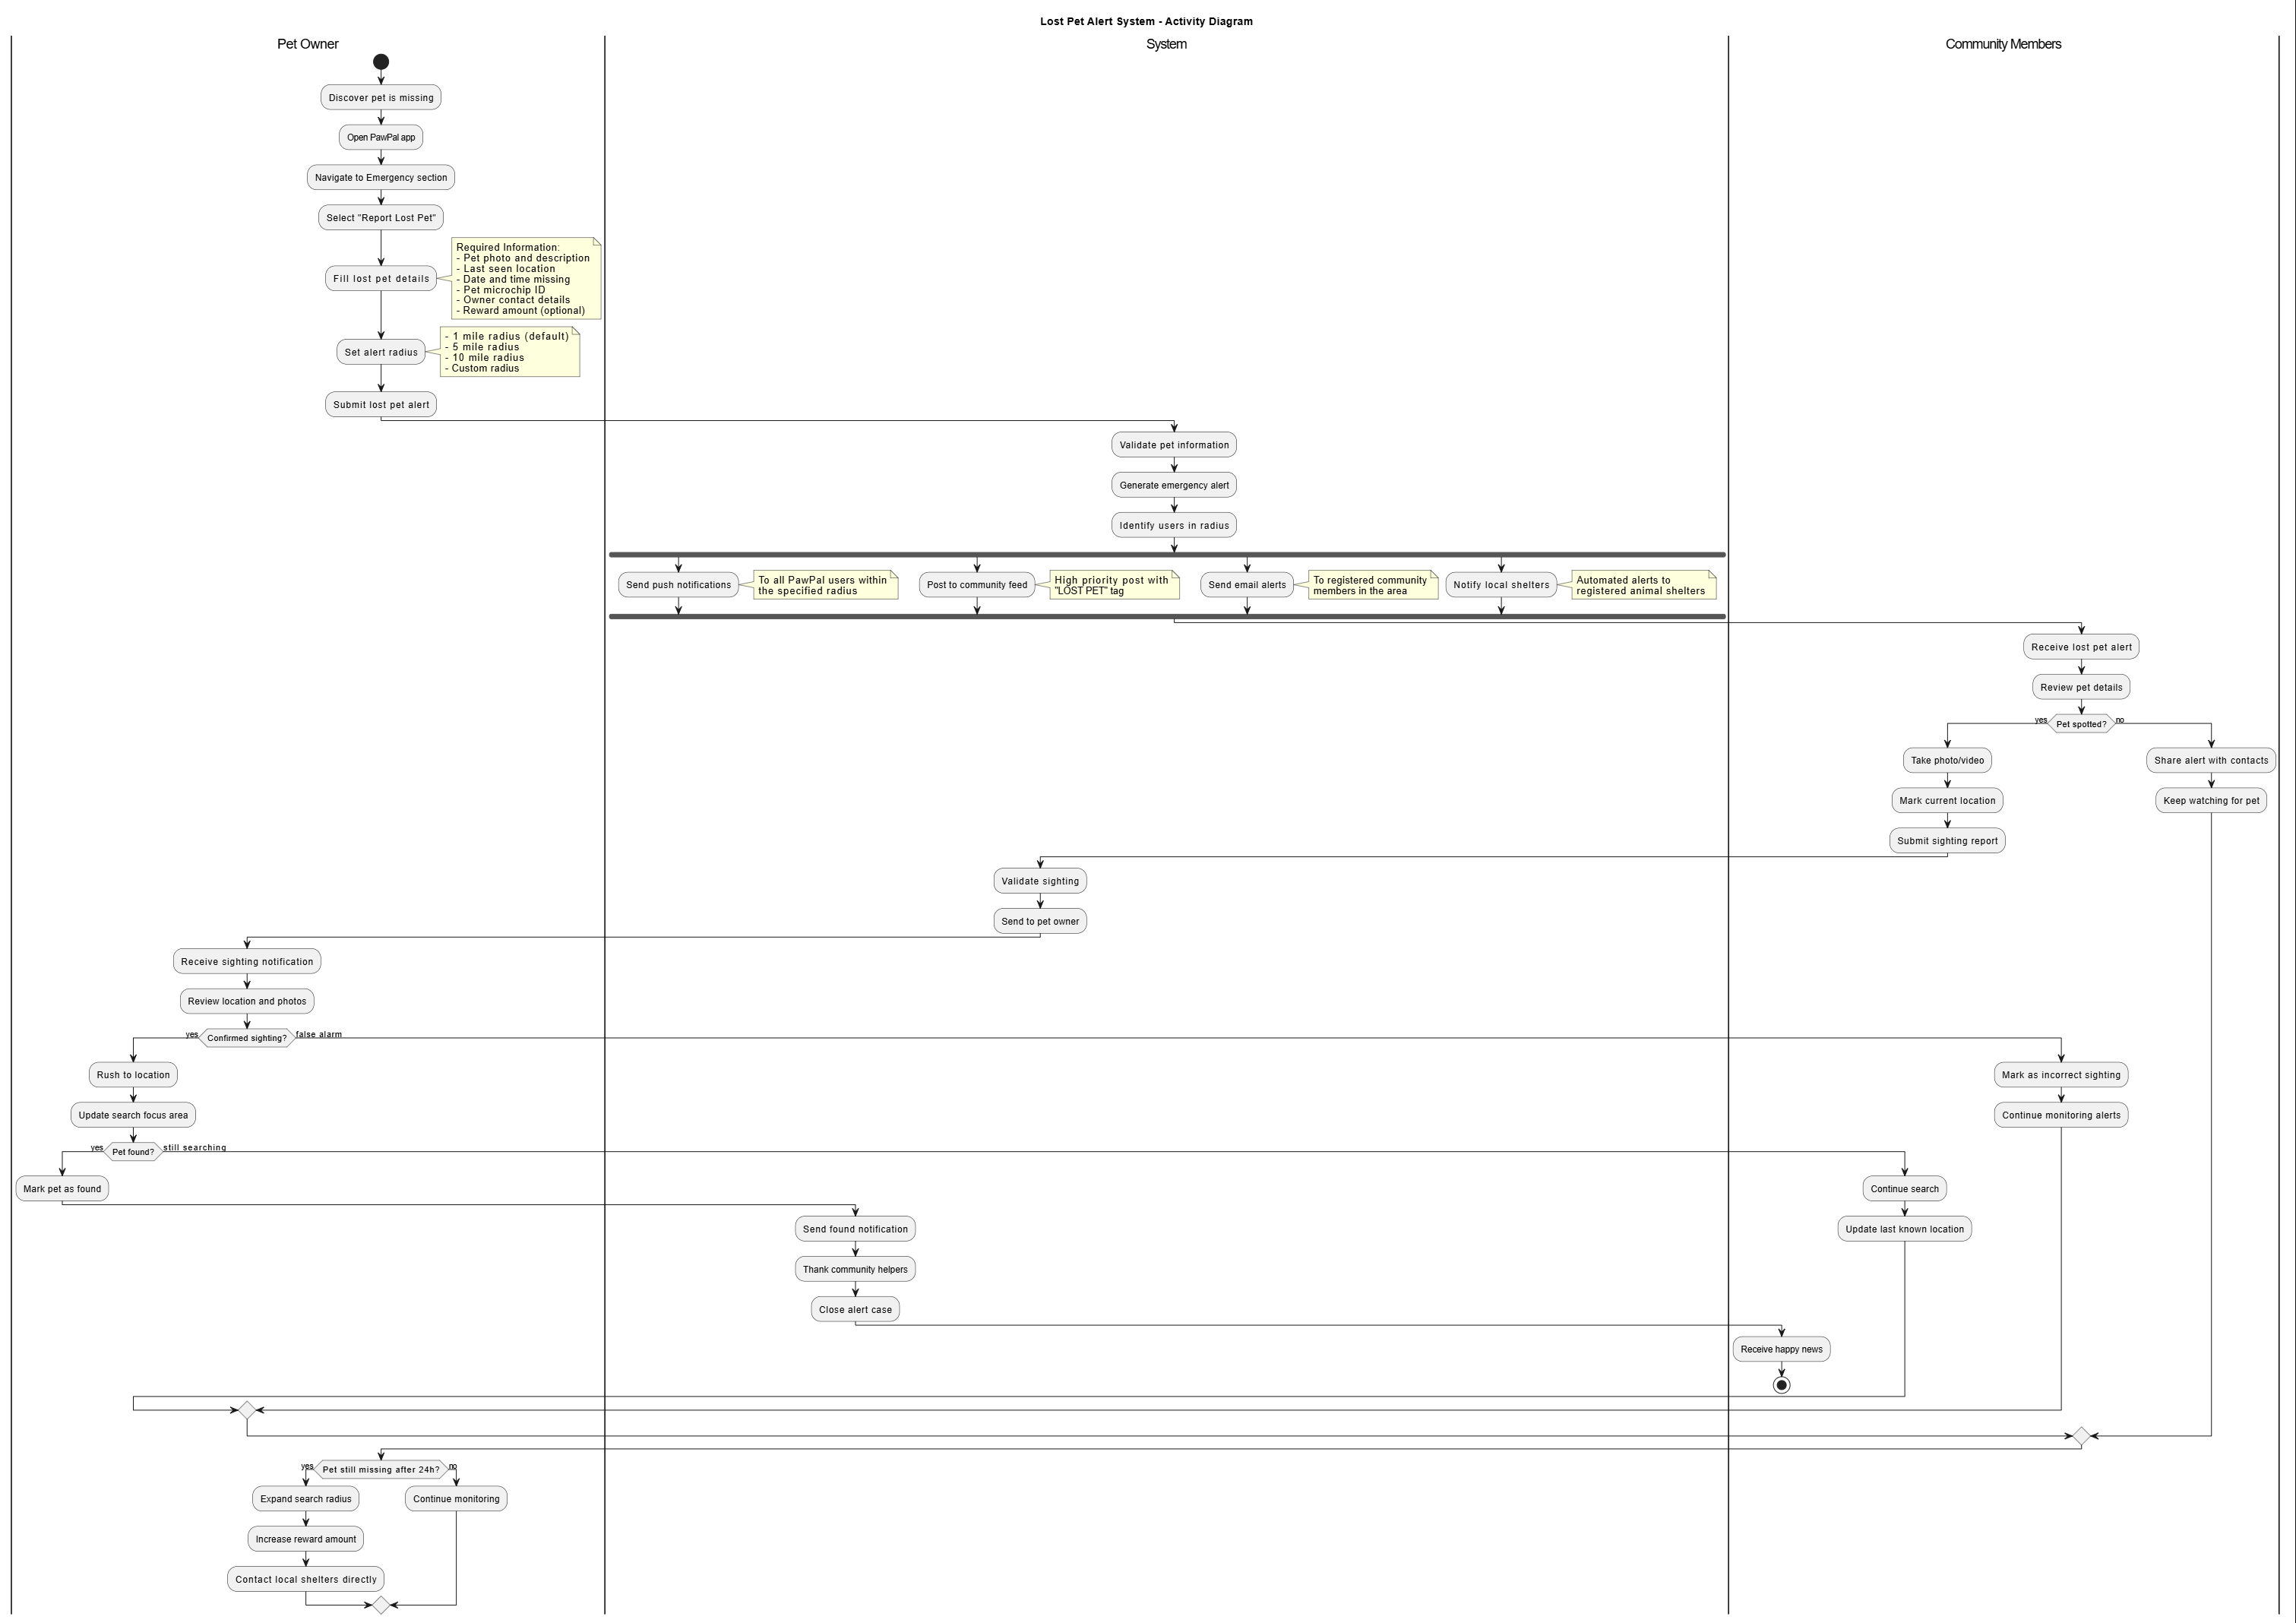
\includegraphics[width=1.0\textwidth]{ThesisFigs/activity_lost_pet_alert.png}
    \caption{Lost Pet Alert Activity Diagram}
    \label{fig:activity_lost_pet_alert}
\end{figure}

This activity diagram shows the emergency lost pet alert system workflow including alert creation with pet details and last known location, radius-based community notifications via push notifications and email, shelter alert distribution, sighting reporting with photo verification, and case resolution tracking.

\subsubsection{Pet Adoption Process}

\begin{figure}[H]
    \centering
    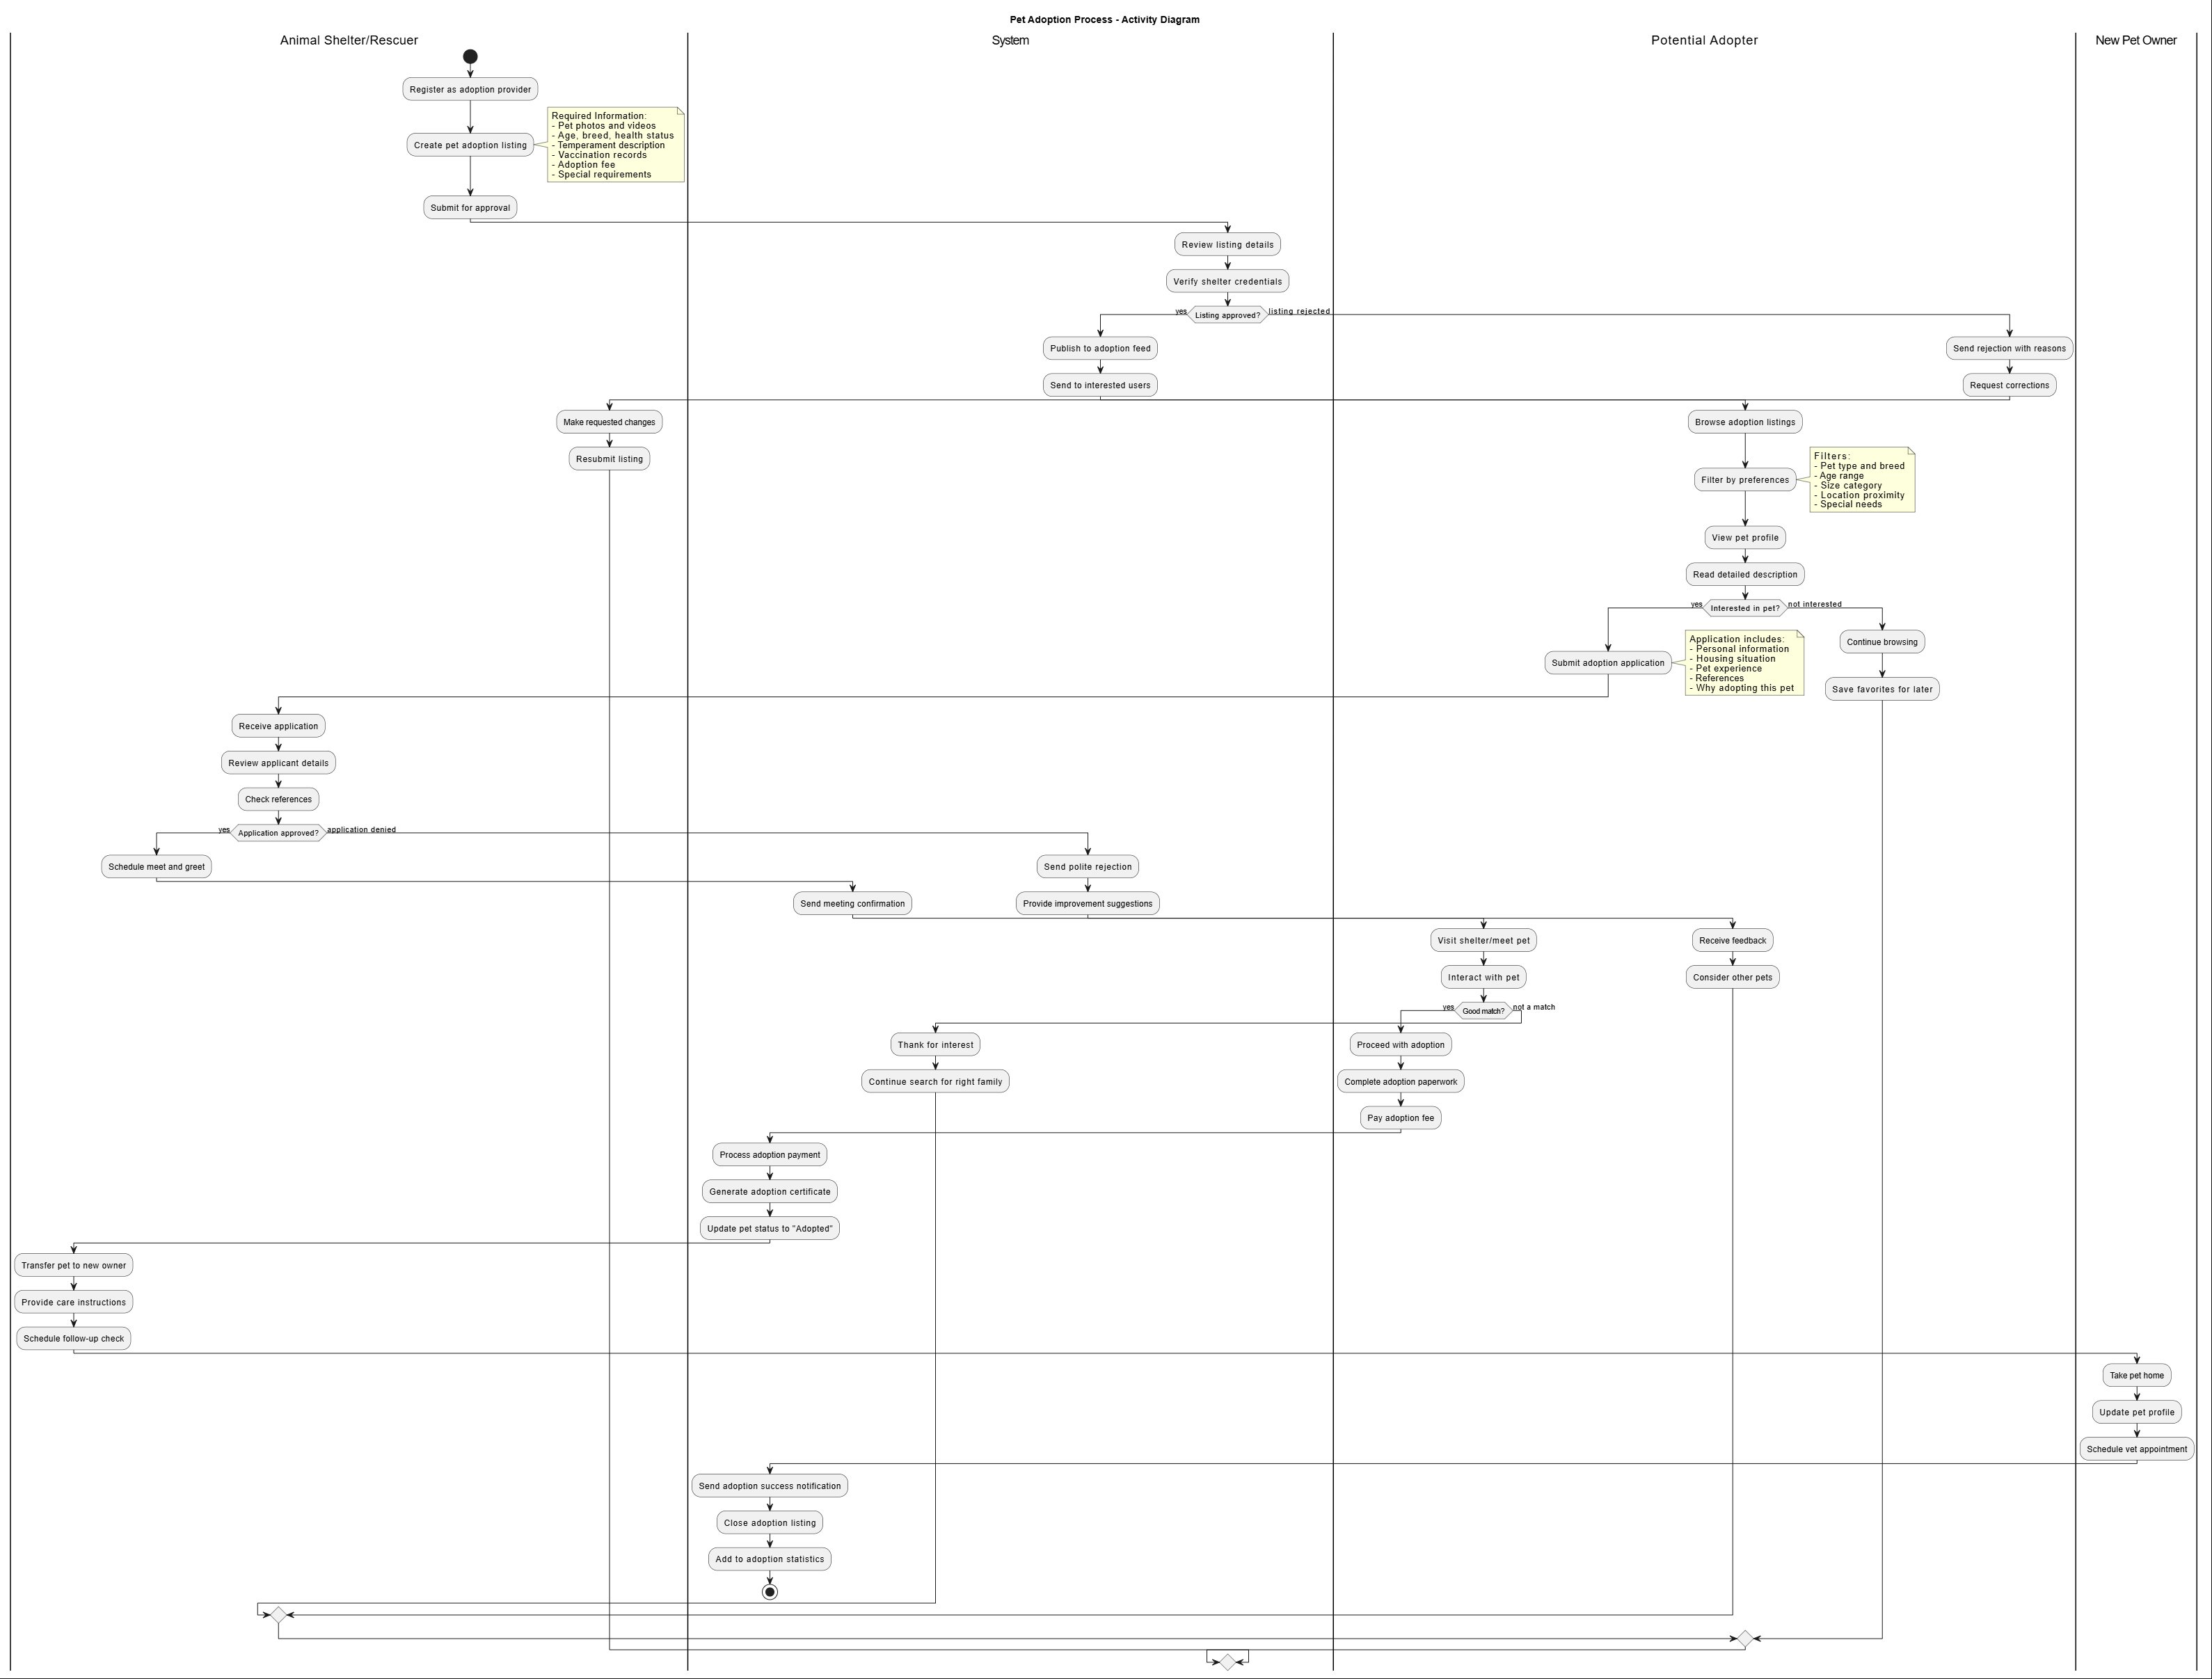
\includegraphics[width=0.9\textwidth]{ThesisFigs/activity_pet_adoption.png}
    \caption{Pet Adoption Process Activity Diagram}
    \label{fig:activity_pet_adoption}
\end{figure}

This comprehensive activity diagram models the pet adoption process from shelter registration through successful adoption. The flow includes shelter verification, pet profile creation with health records, adoption application screening, background checks, meet-and-greet scheduling, and adoption finalization with legal documentation.

\subsection{Class Diagram: Core Domain Model}

\begin{figure}[htbp]
    \centering
    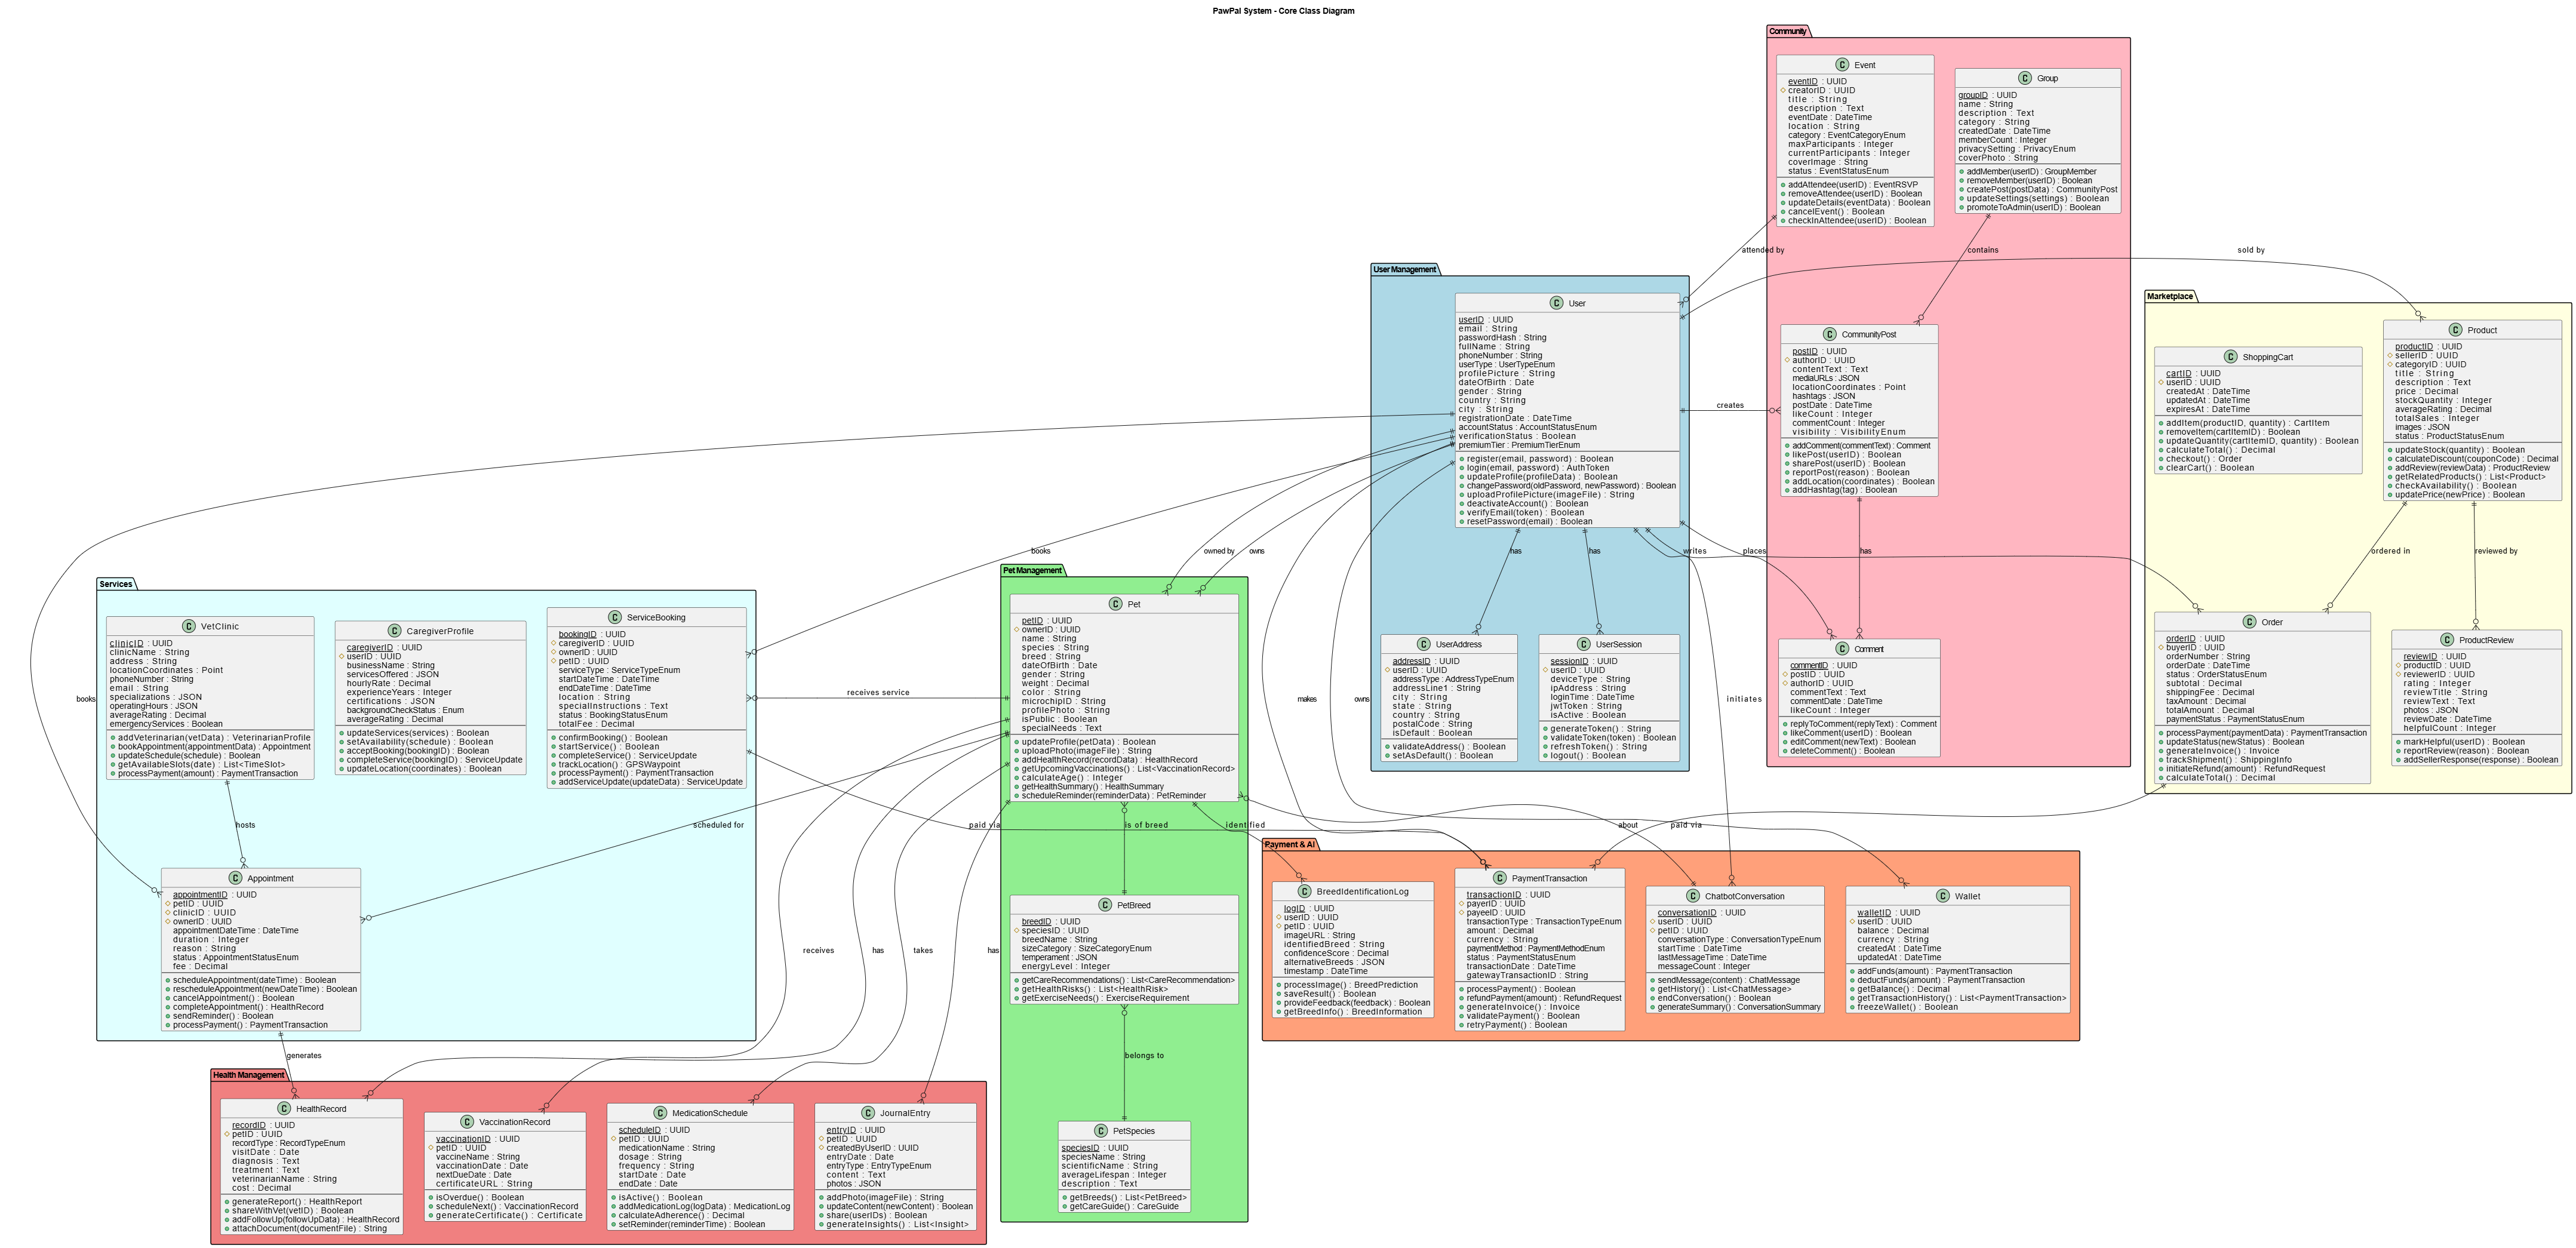
\includegraphics[width=0.95\textwidth]{ThesisFigs/class_diagram.png}
    \caption{PawPal System - Core Class Diagram}
    \label{fig:class_diagram}
\end{figure}

The class diagram represents the static structure of PawPal's domain model, showing entity relationships, attributes, and key methods. The diagram includes all major entities from the domain model with proper cardinalities indicating one-to-many and many-to-many relationships. Key classes include User, Pet, HealthRecord, Product, Order, Appointment, ServiceBooking, PaymentTransaction, CommunityPost, and ChatbotConversation with their respective attributes and methods.

\subsection{Sequence Diagrams}

\subsubsection{AI Breed Identification Process}

\begin{figure}[H]
    \centering
    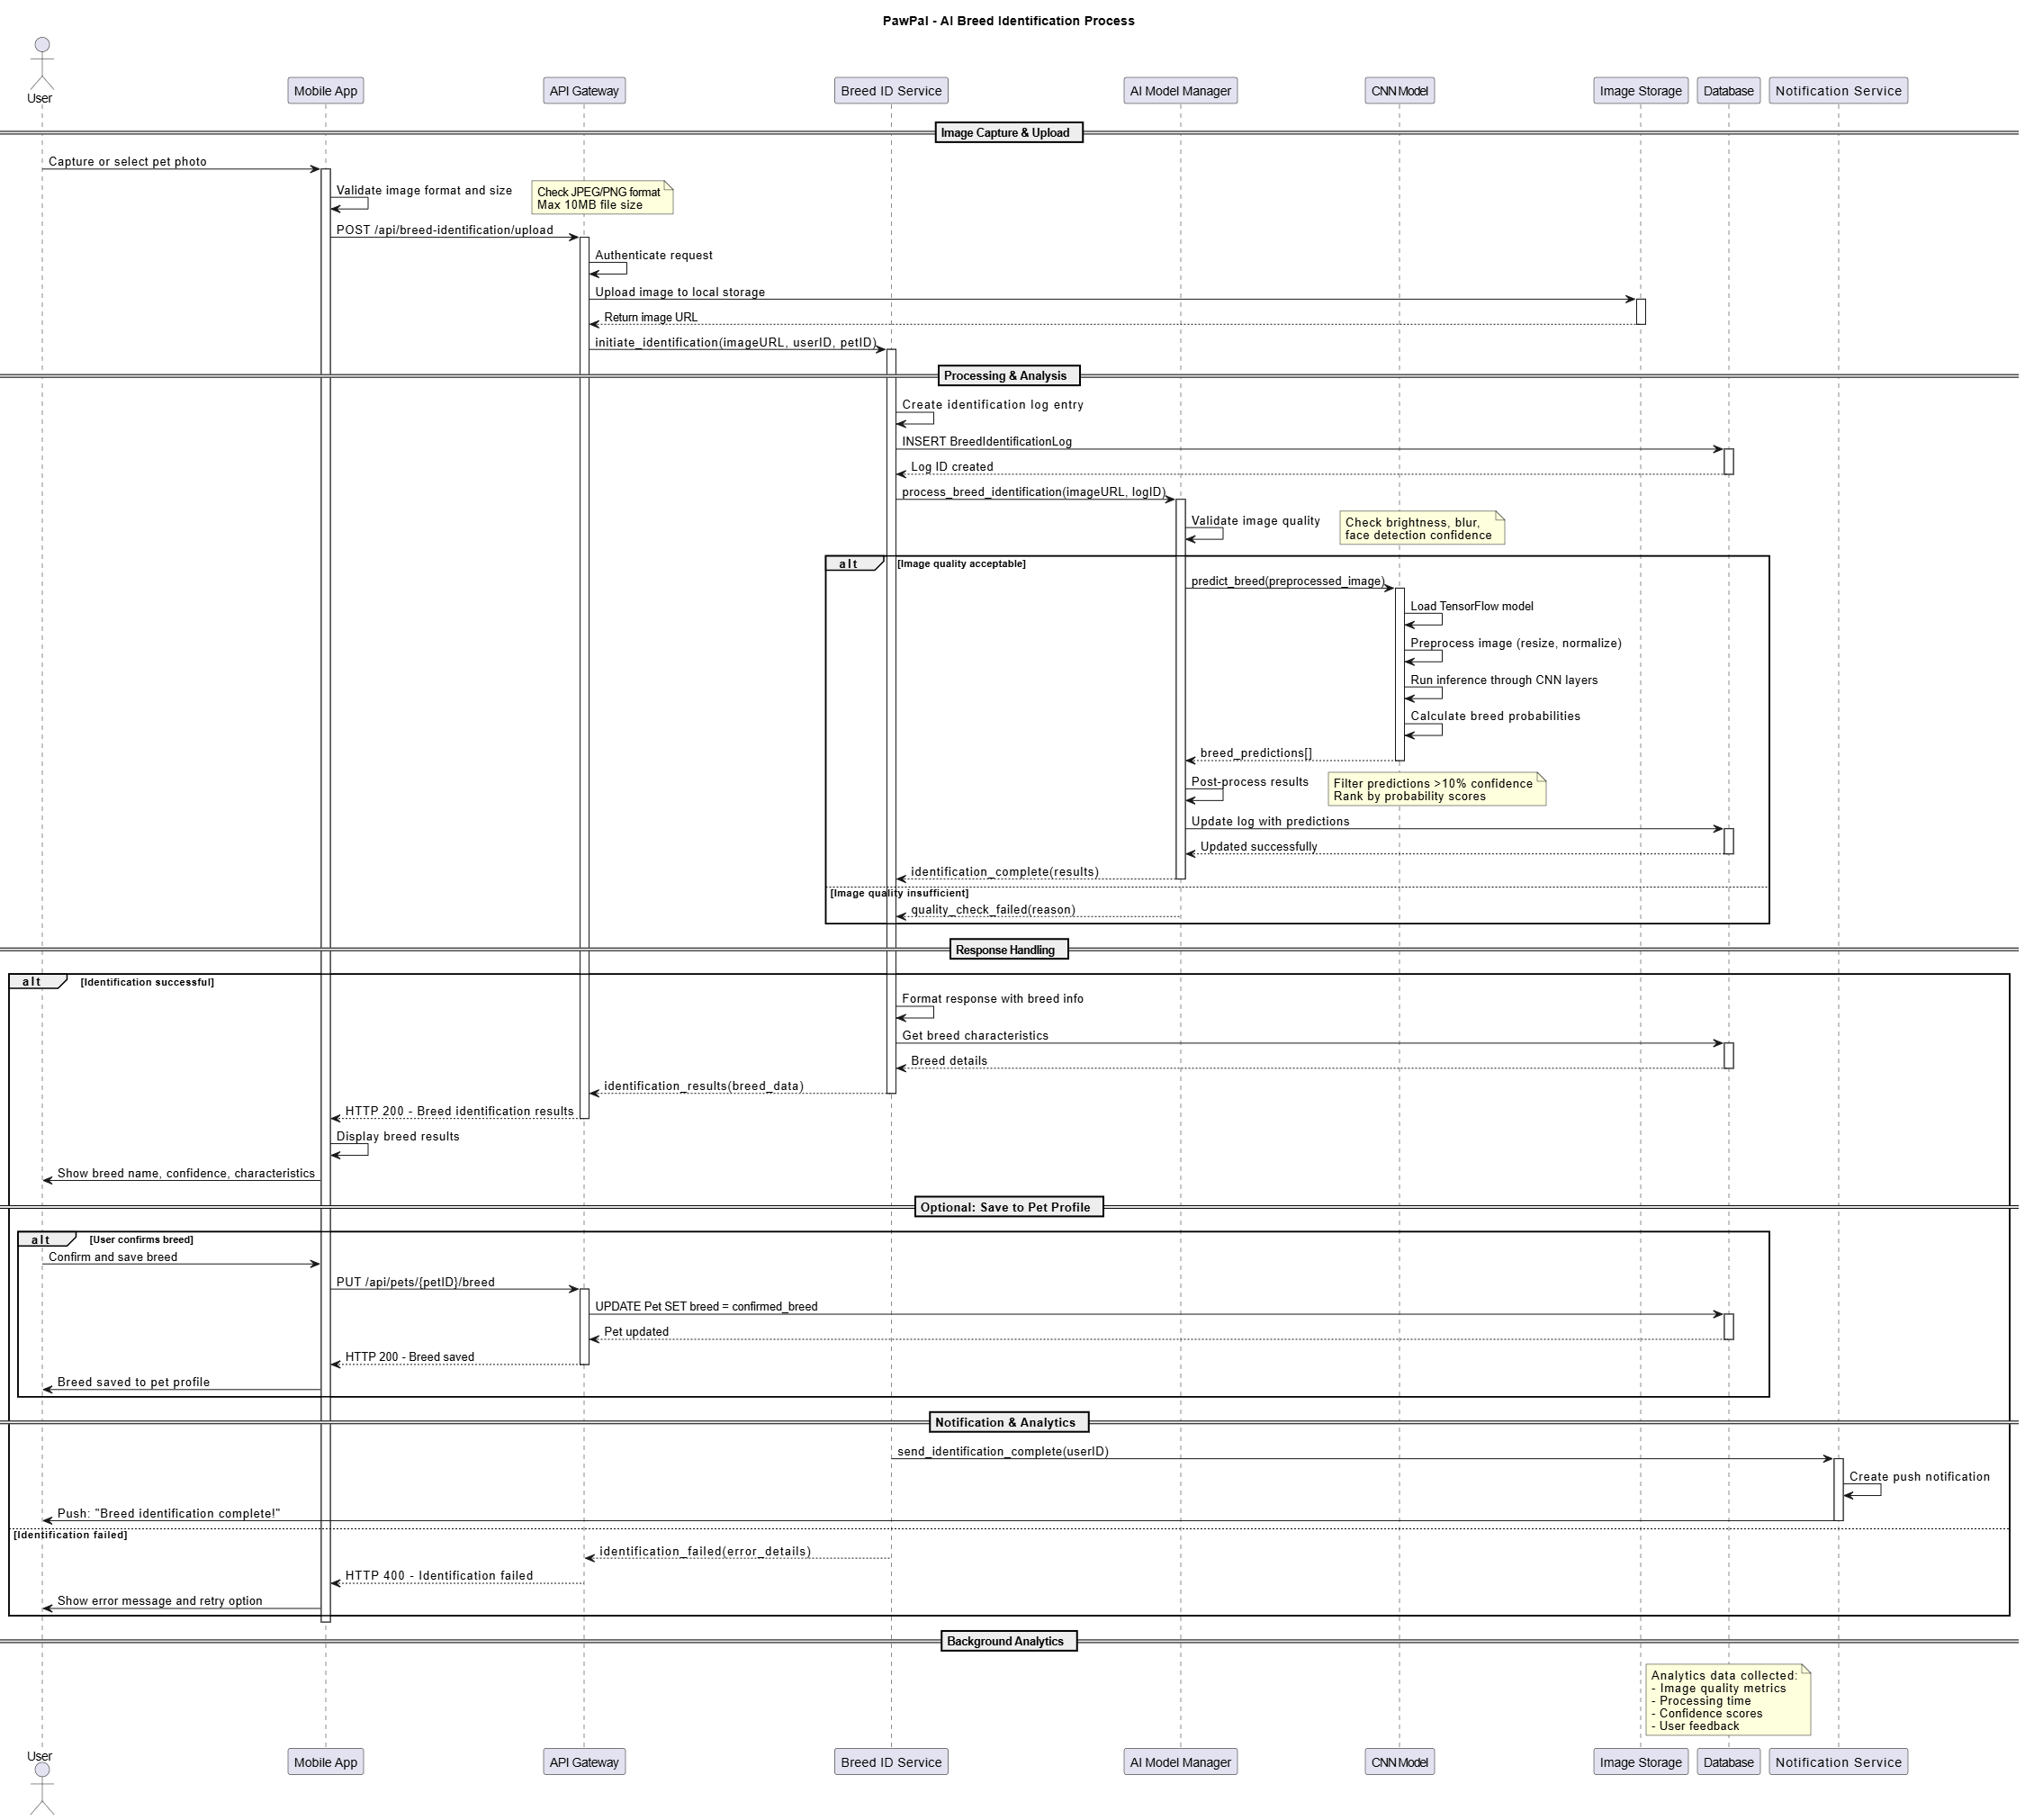
\includegraphics[width=1.0\textwidth]{ThesisFigs/sequence_breed_identification.png}
    \caption{AI Breed Identification Process Sequence Diagram}
    \label{fig:sequence_breed_identification}
\end{figure}

This sequence diagram illustrates the temporal flow of breed identification, showing interaction between user interface, API gateway, breed identification service, AI model manager, CNN model, and database. The diagram emphasizes image quality validation, model inference, and result logging within the unified application.

\subsubsection{Payment Processing Flow}

\begin{figure}[H]
    \centering
    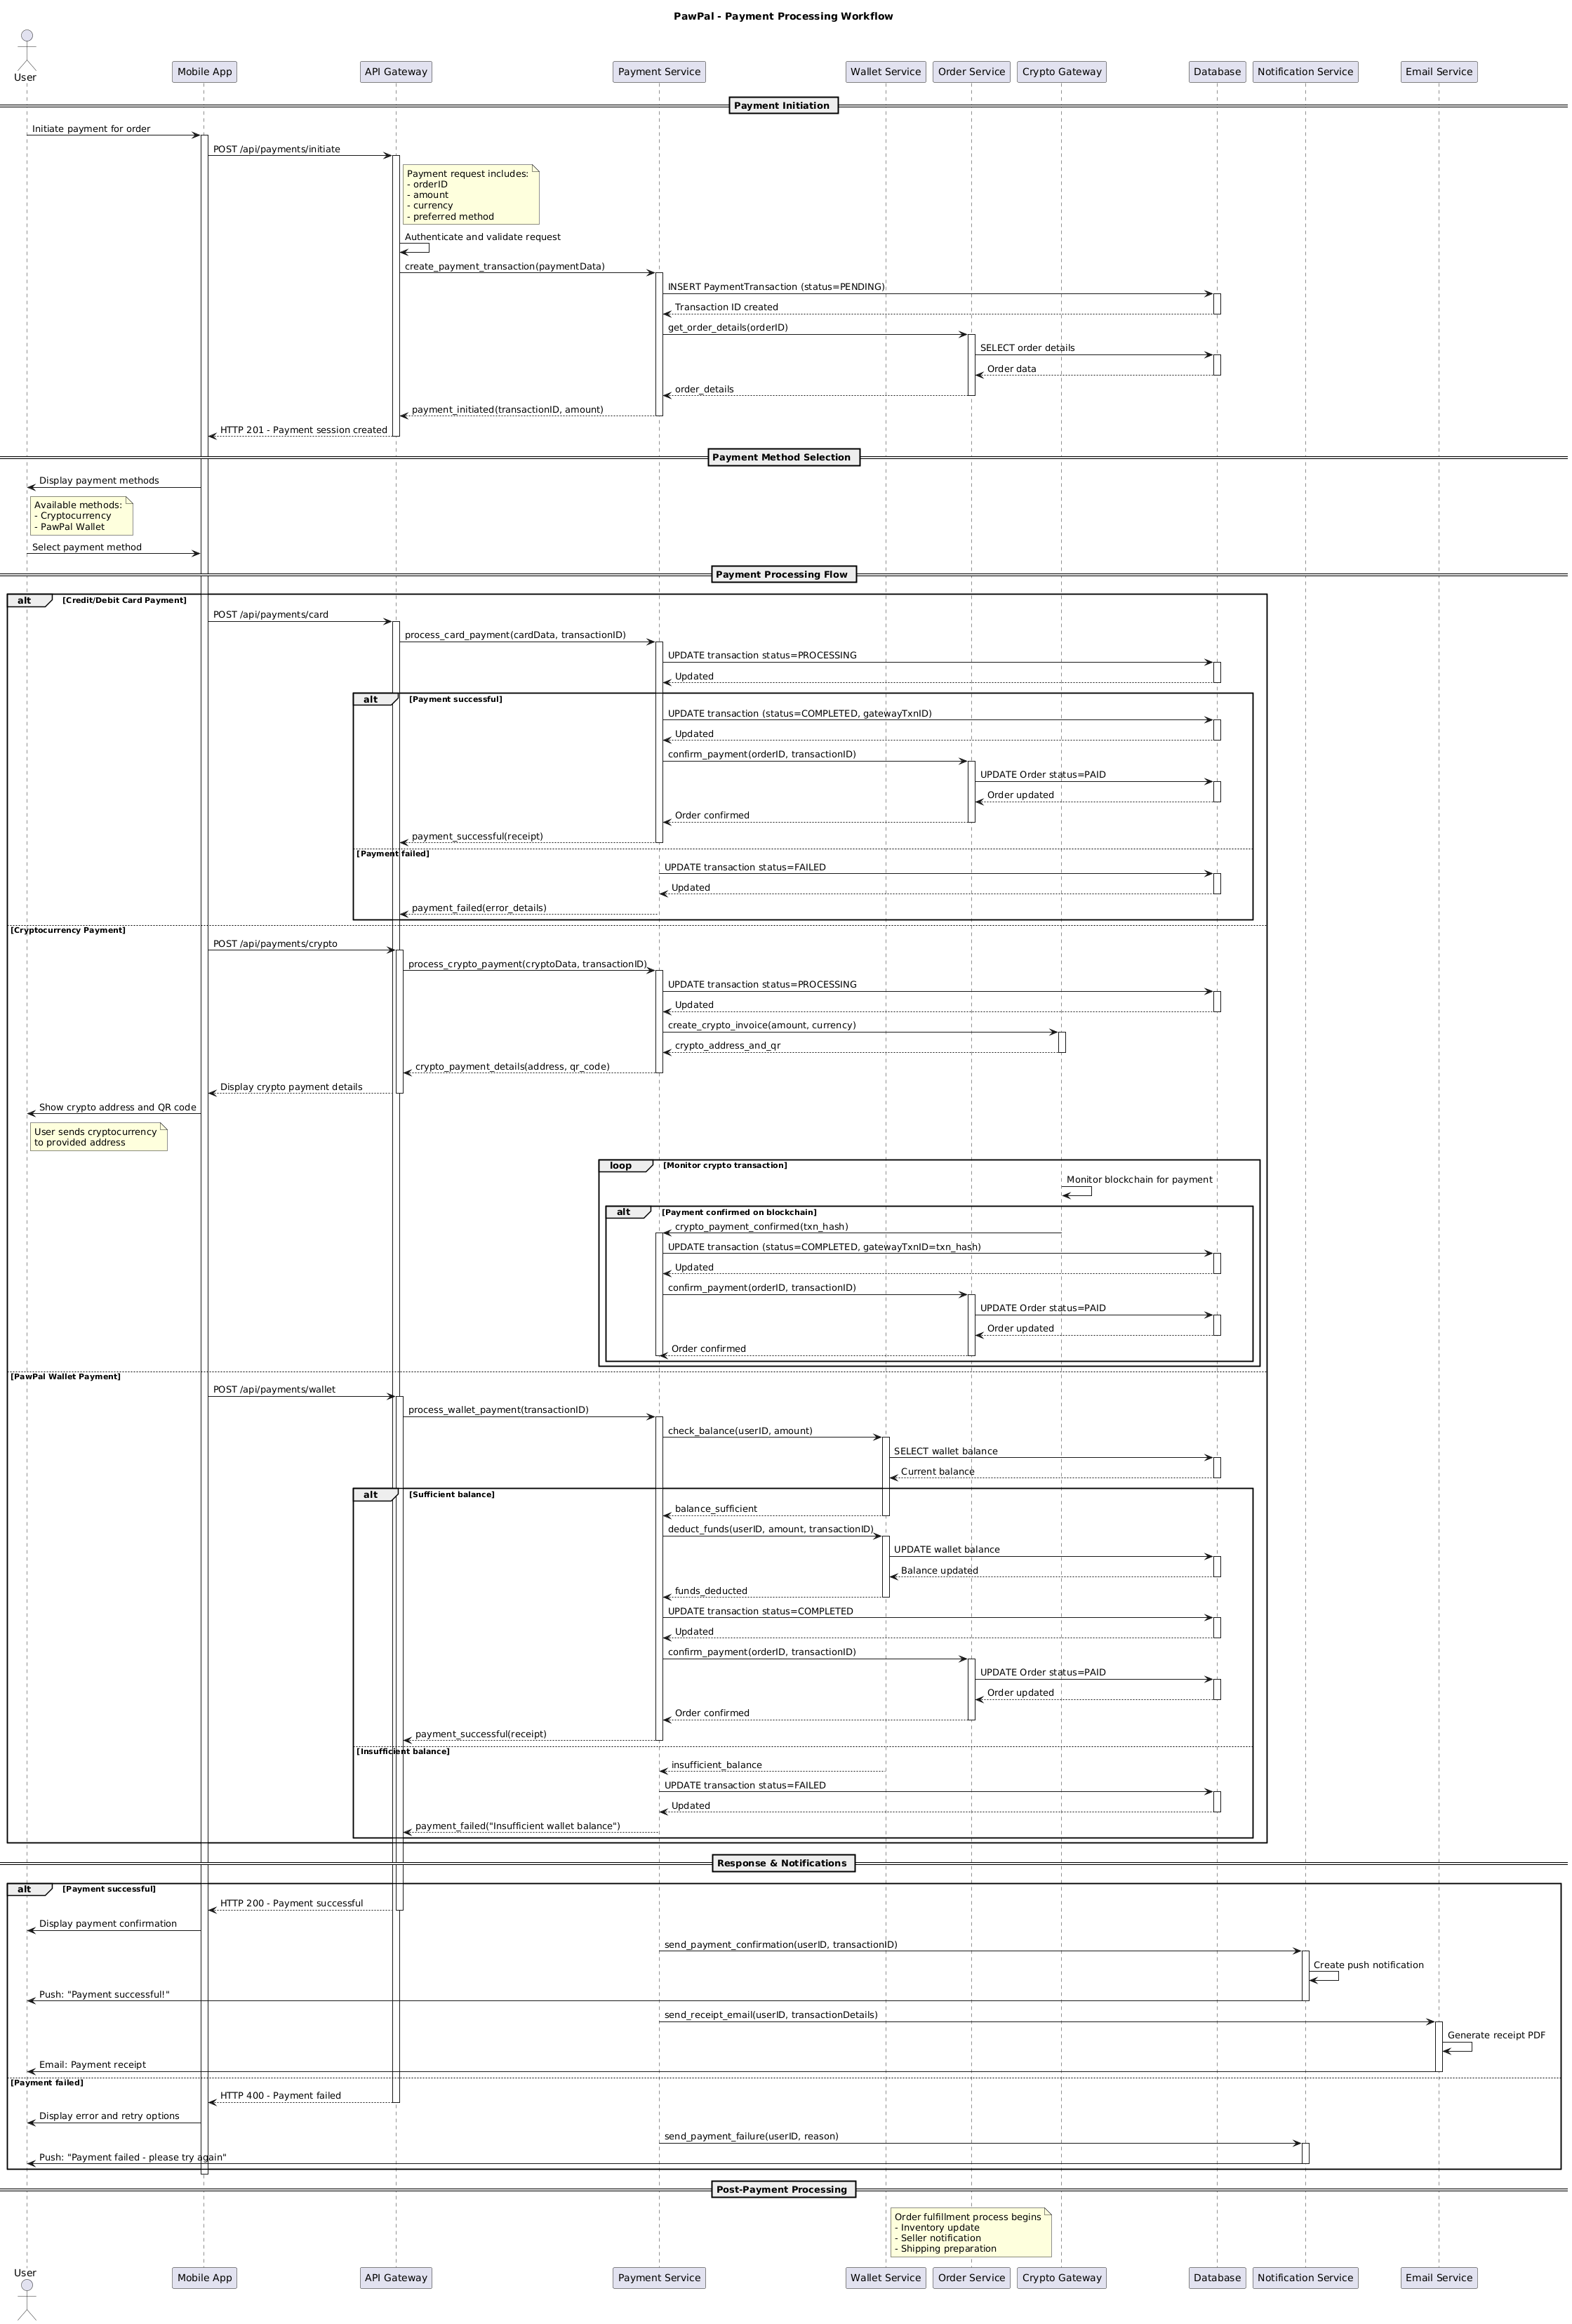
\includegraphics[width=1.0\textwidth]{ThesisFigs/sequence_payment_processing.png}
    \caption{Payment Processing Workflow Sequence Diagram}
    \label{fig:sequence_payment_processing}
\end{figure}

This critical sequence diagram models the payment processing workflow with alternative flows for different payment methods (card, crypto, wallet) and handles success/failure scenarios. It demonstrates direct module-to-module function calls within the monolithic application, enabling atomic transactions across Payment, Order, and Notification modules.

\subsubsection{Veterinary Appointment Booking}

\begin{figure}[H]
    \centering
    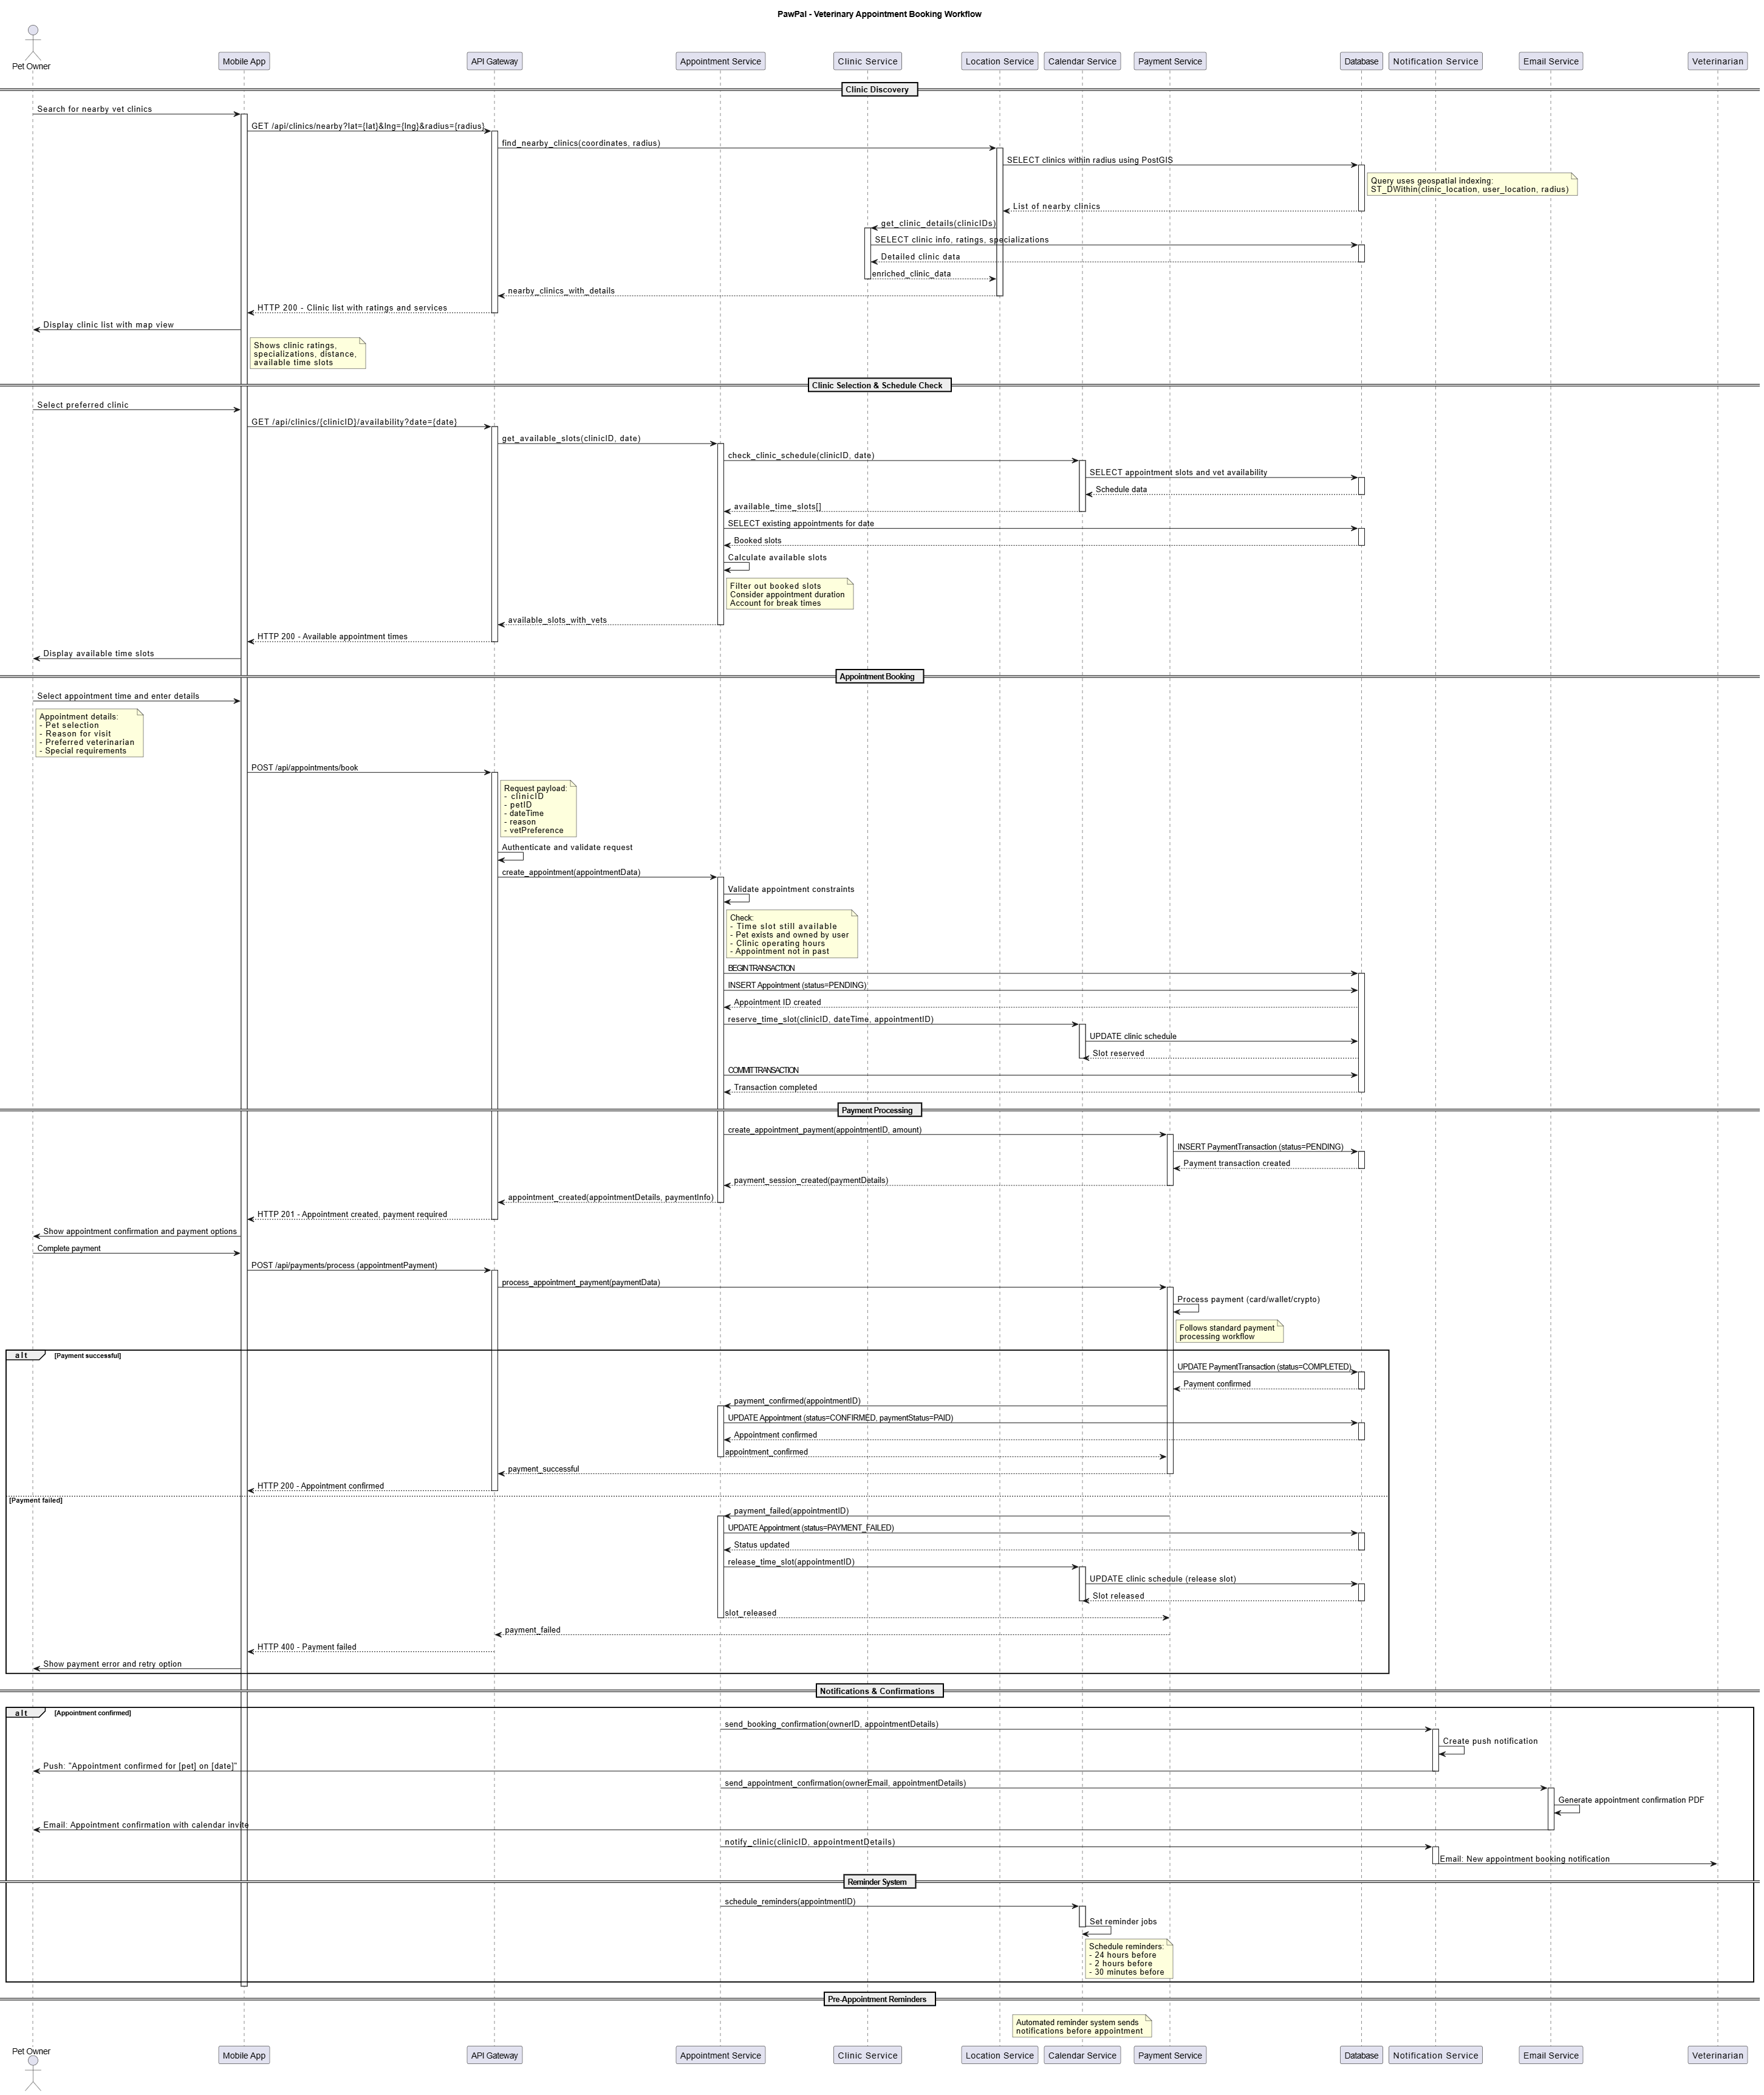
\includegraphics[width=1.0\textwidth]{ThesisFigs/sequence_vet_appointment.png}
    \caption{Veterinary Appointment Booking Sequence Diagram}
    \label{fig:sequence_vet_appointment}
\end{figure}

This sequence diagram shows the complete appointment booking workflow including clinic discovery using geospatial queries, availability checking, booking creation, payment processing, and confirmation notifications to both pet owner and veterinary clinic.

\subsubsection{Community Post Creation with Real-time Updates}

\begin{figure}[H]
    \centering
    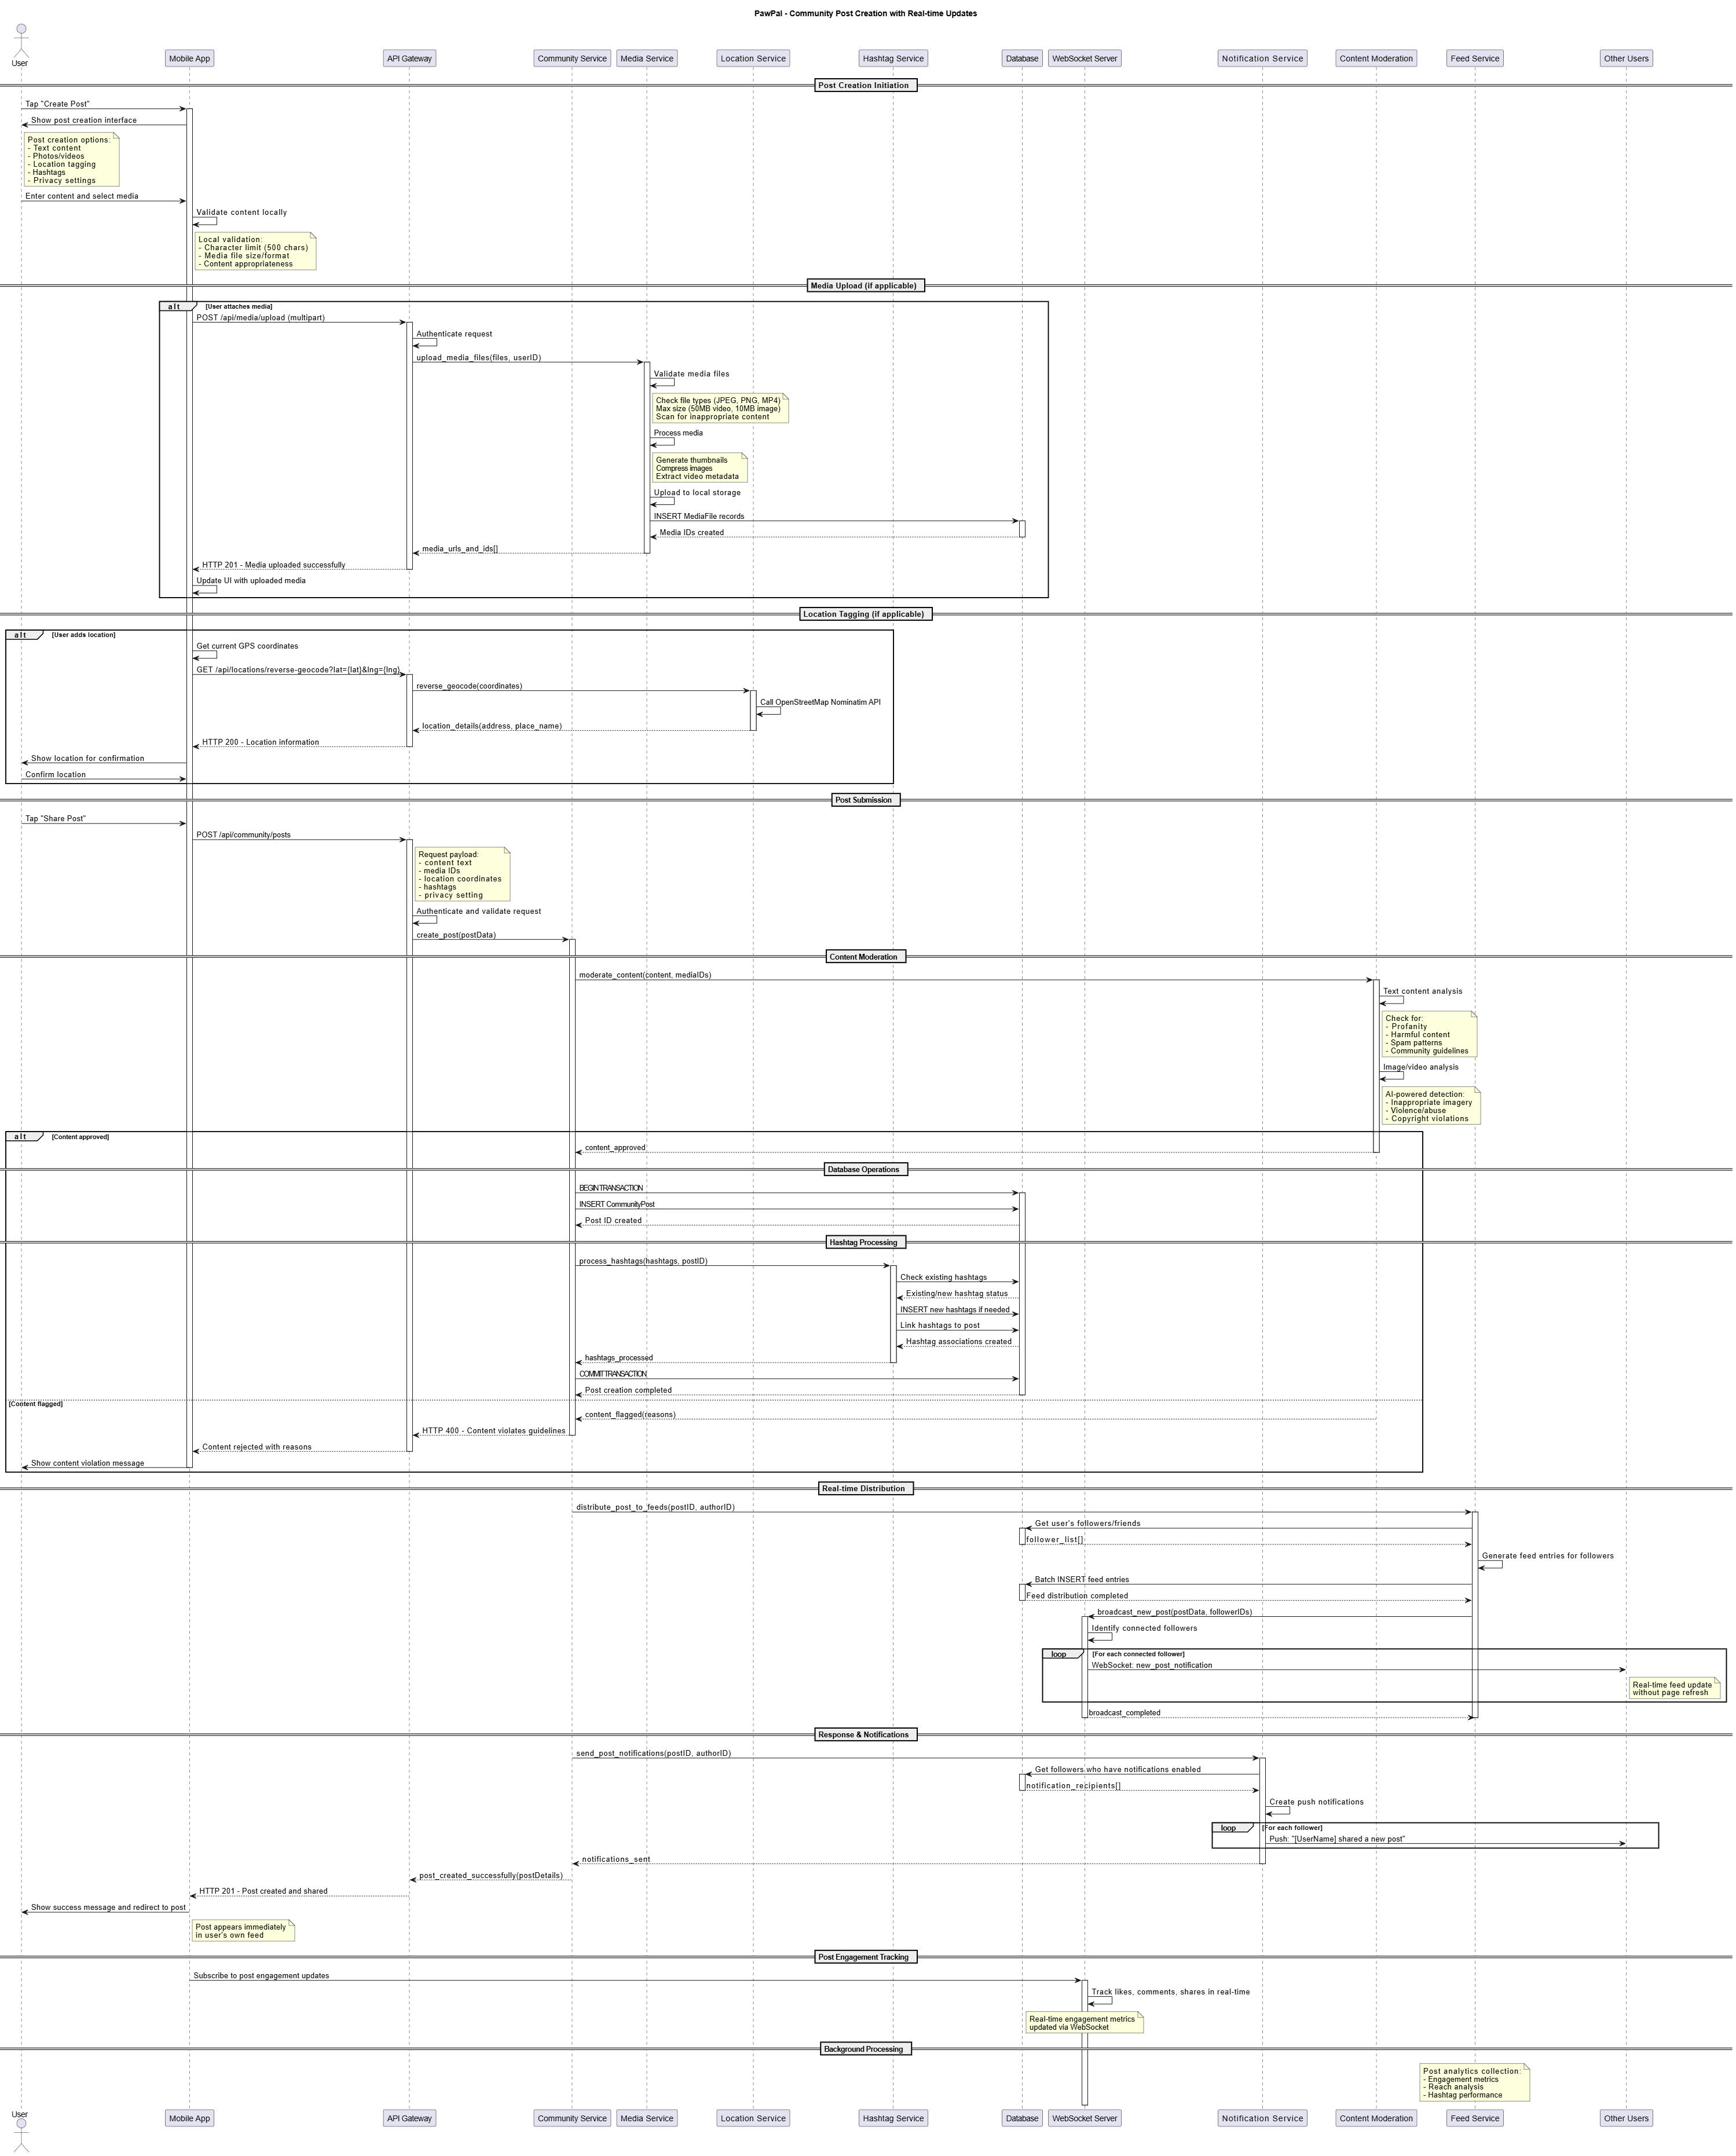
\includegraphics[width=1.0\textwidth]{ThesisFigs/sequence_community_post.png}
    \caption{Community Post Creation Sequence Diagram}
    \label{fig:sequence_community_post}
\end{figure}

This sequence diagram illustrates the community post creation process including media upload, content moderation, hashtag processing, real-time distribution to followers via WebSocket, and push notification delivery for enhanced user engagement.

\subsubsection{Caregiver GPS Tracking System}

\begin{figure}[H]
    \centering
    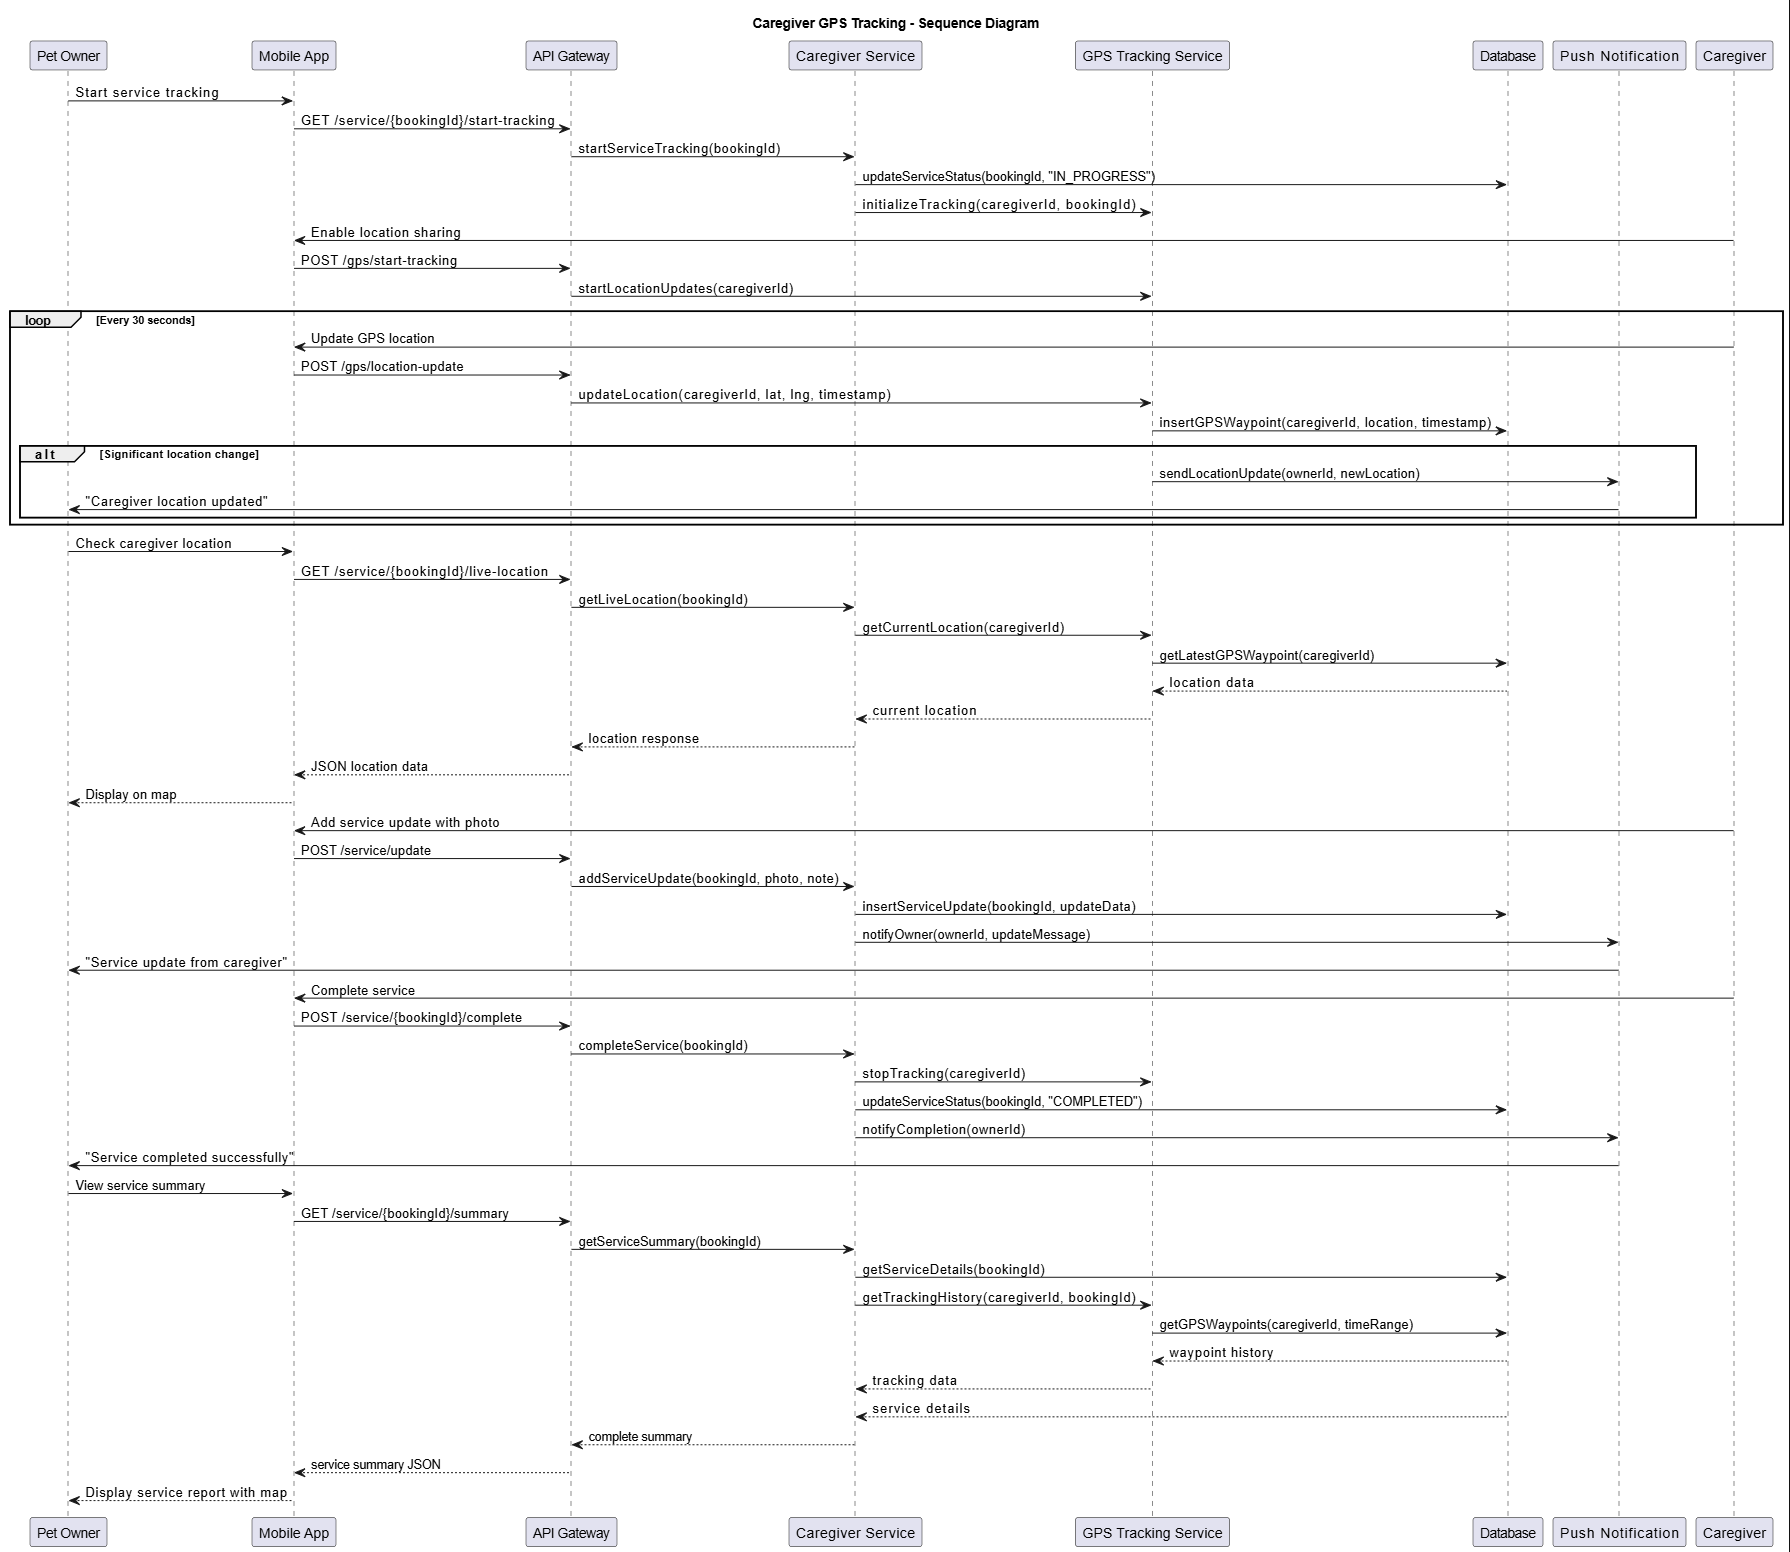
\includegraphics[width=1.0\textwidth]{ThesisFigs/sequence_caregiver_gps_tracking.png}
    \caption{Caregiver GPS Tracking Sequence Diagram}
    \label{fig:sequence_caregiver_gps_tracking}
\end{figure}

This sequence diagram demonstrates the real-time GPS tracking system for caregiver services, showing continuous location updates, service progress reporting with photos, and comprehensive service completion tracking. The workflow emphasizes real-time communication and transparency during service delivery.

\subsubsection{AI Chatbot RAG Pipeline}

\begin{figure}[H]
    \centering
    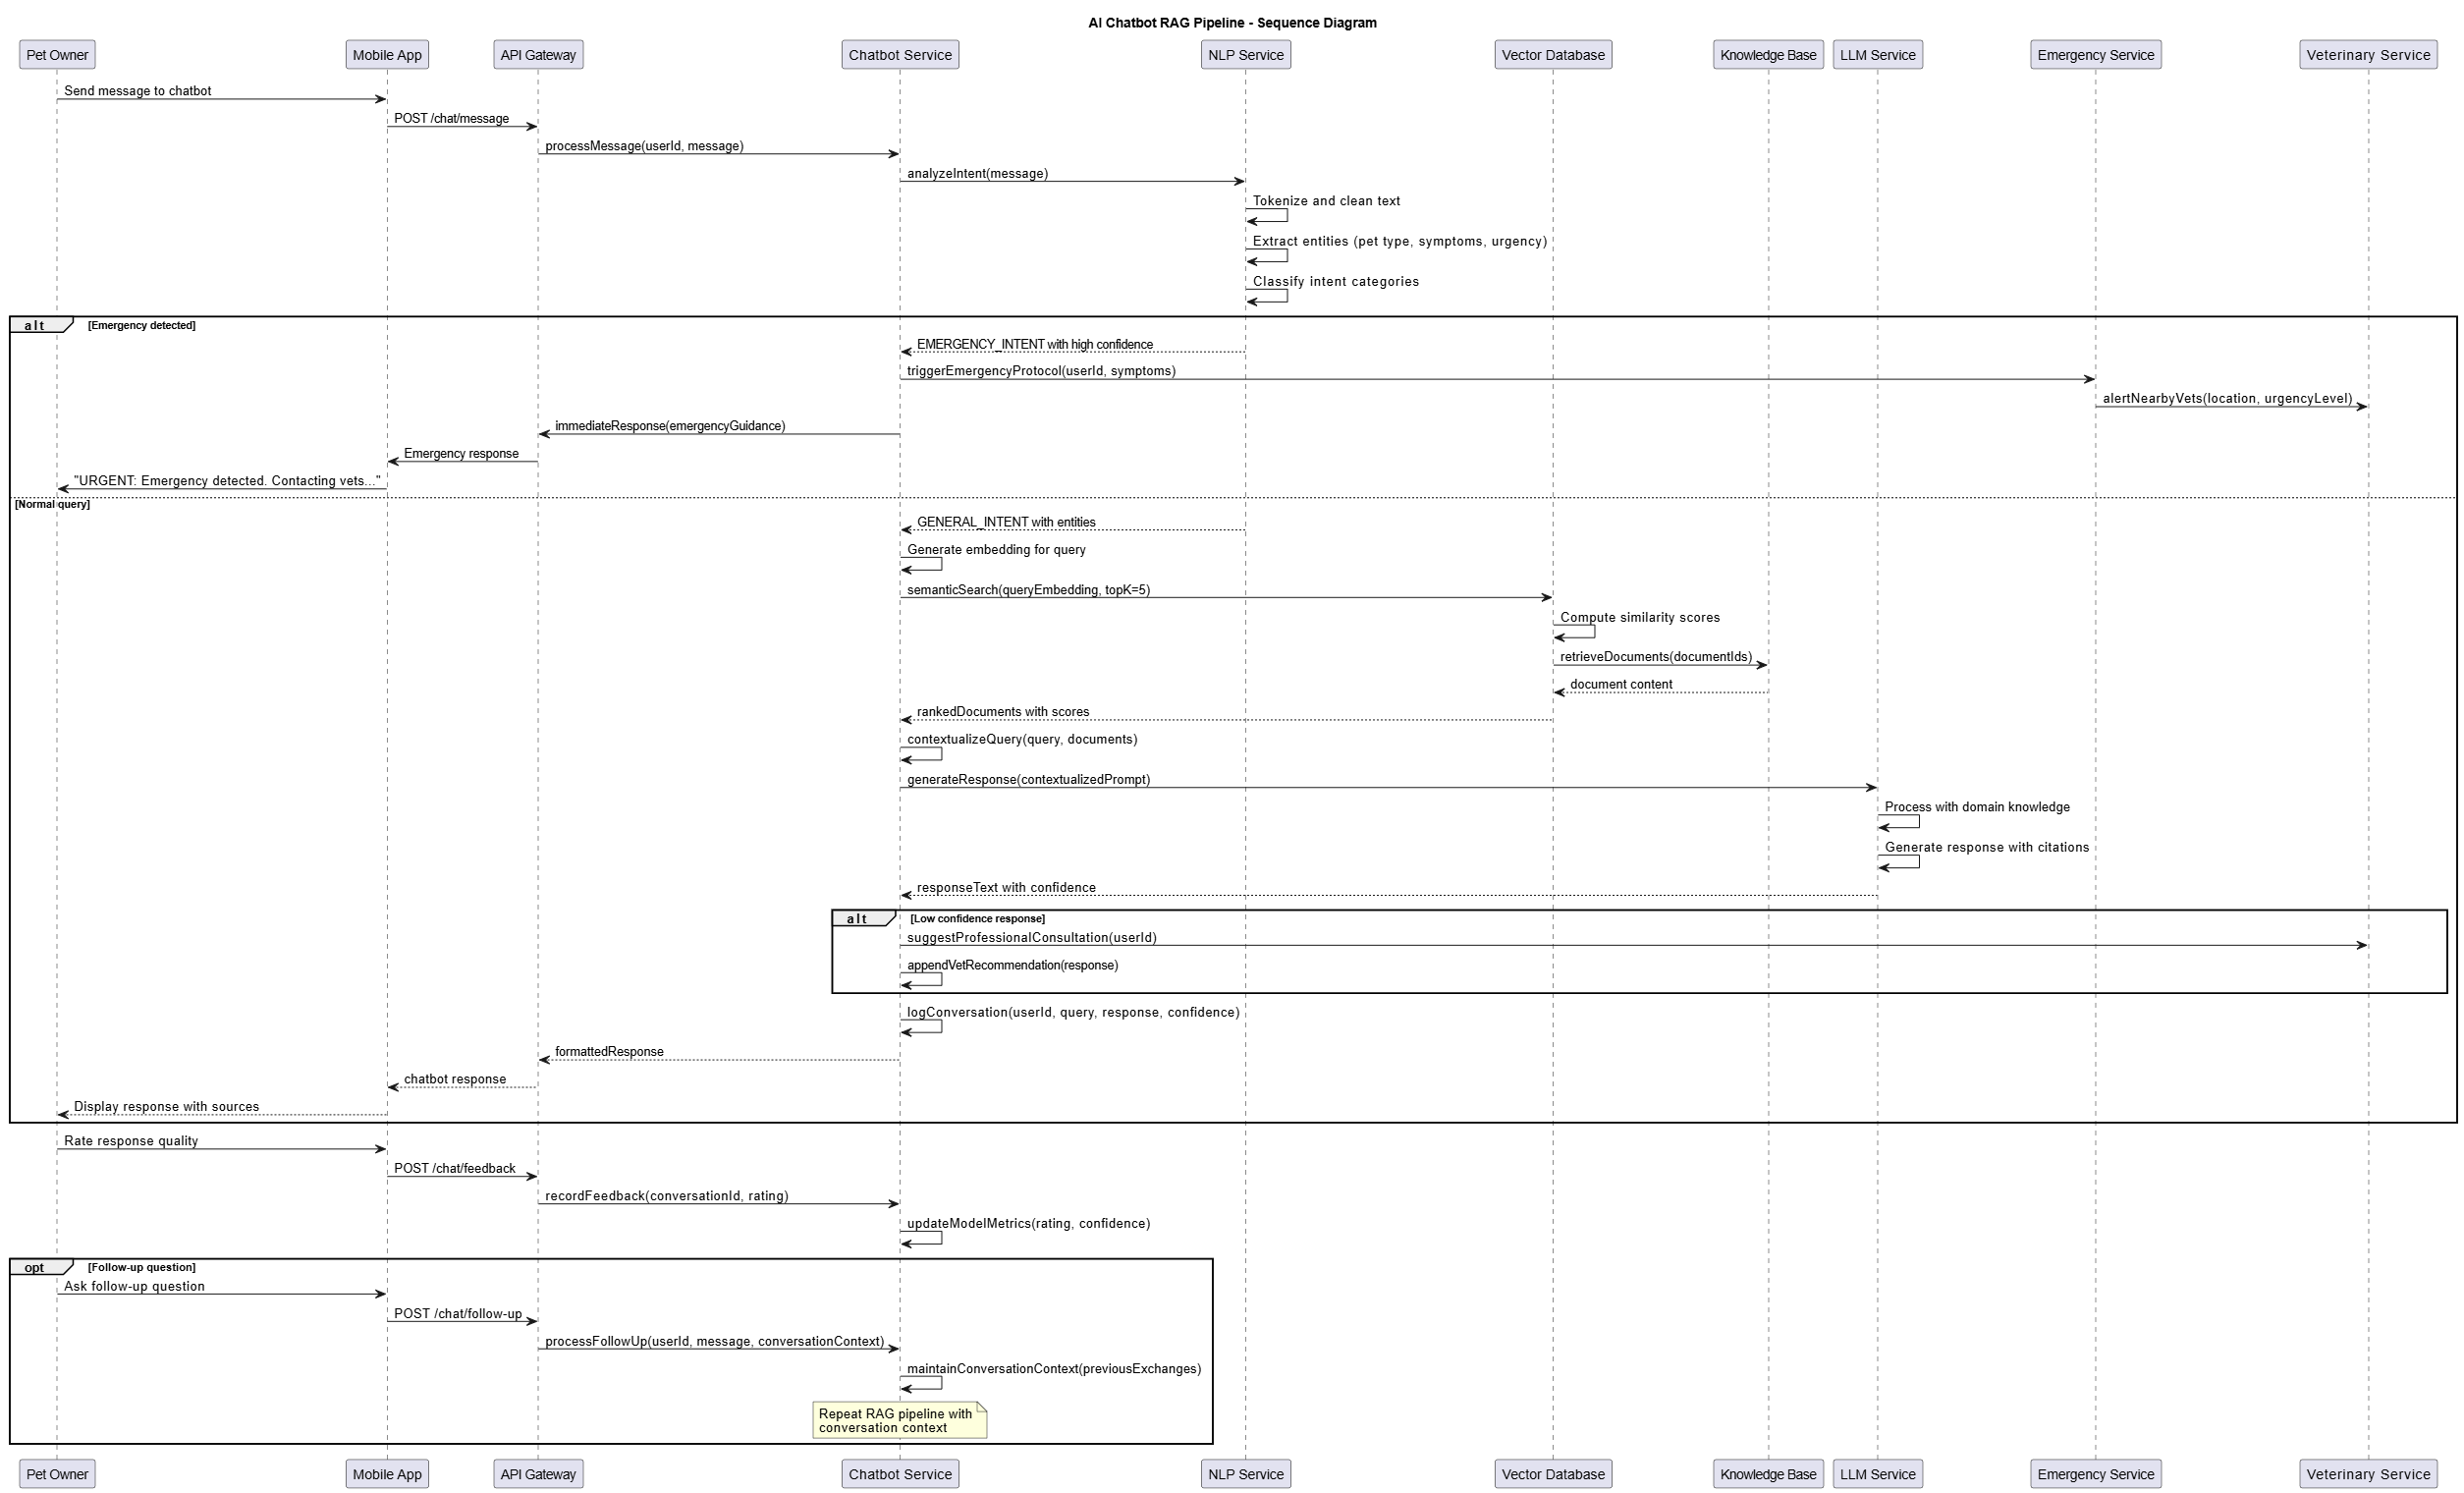
\includegraphics[width=1.0\textwidth]{ThesisFigs/sequence_chatbot_rag_pipeline.png}
    \caption{AI Chatbot RAG Pipeline Sequence Diagram}
    \label{fig:sequence_chatbot_rag_pipeline}
\end{figure}

This critical sequence diagram illustrates the Retrieval-Augmented Generation (RAG) pipeline for the AI chatbot system. The flow includes natural language processing for intent analysis, emergency detection with automatic veterinarian alerts, semantic search through the knowledge base, LLM processing with domain-specific context, and confidence-based response handling with professional consultation recommendations.

\subsubsection{Lost Pet Alert Broadcasting}

\begin{figure}[H]
    \centering
    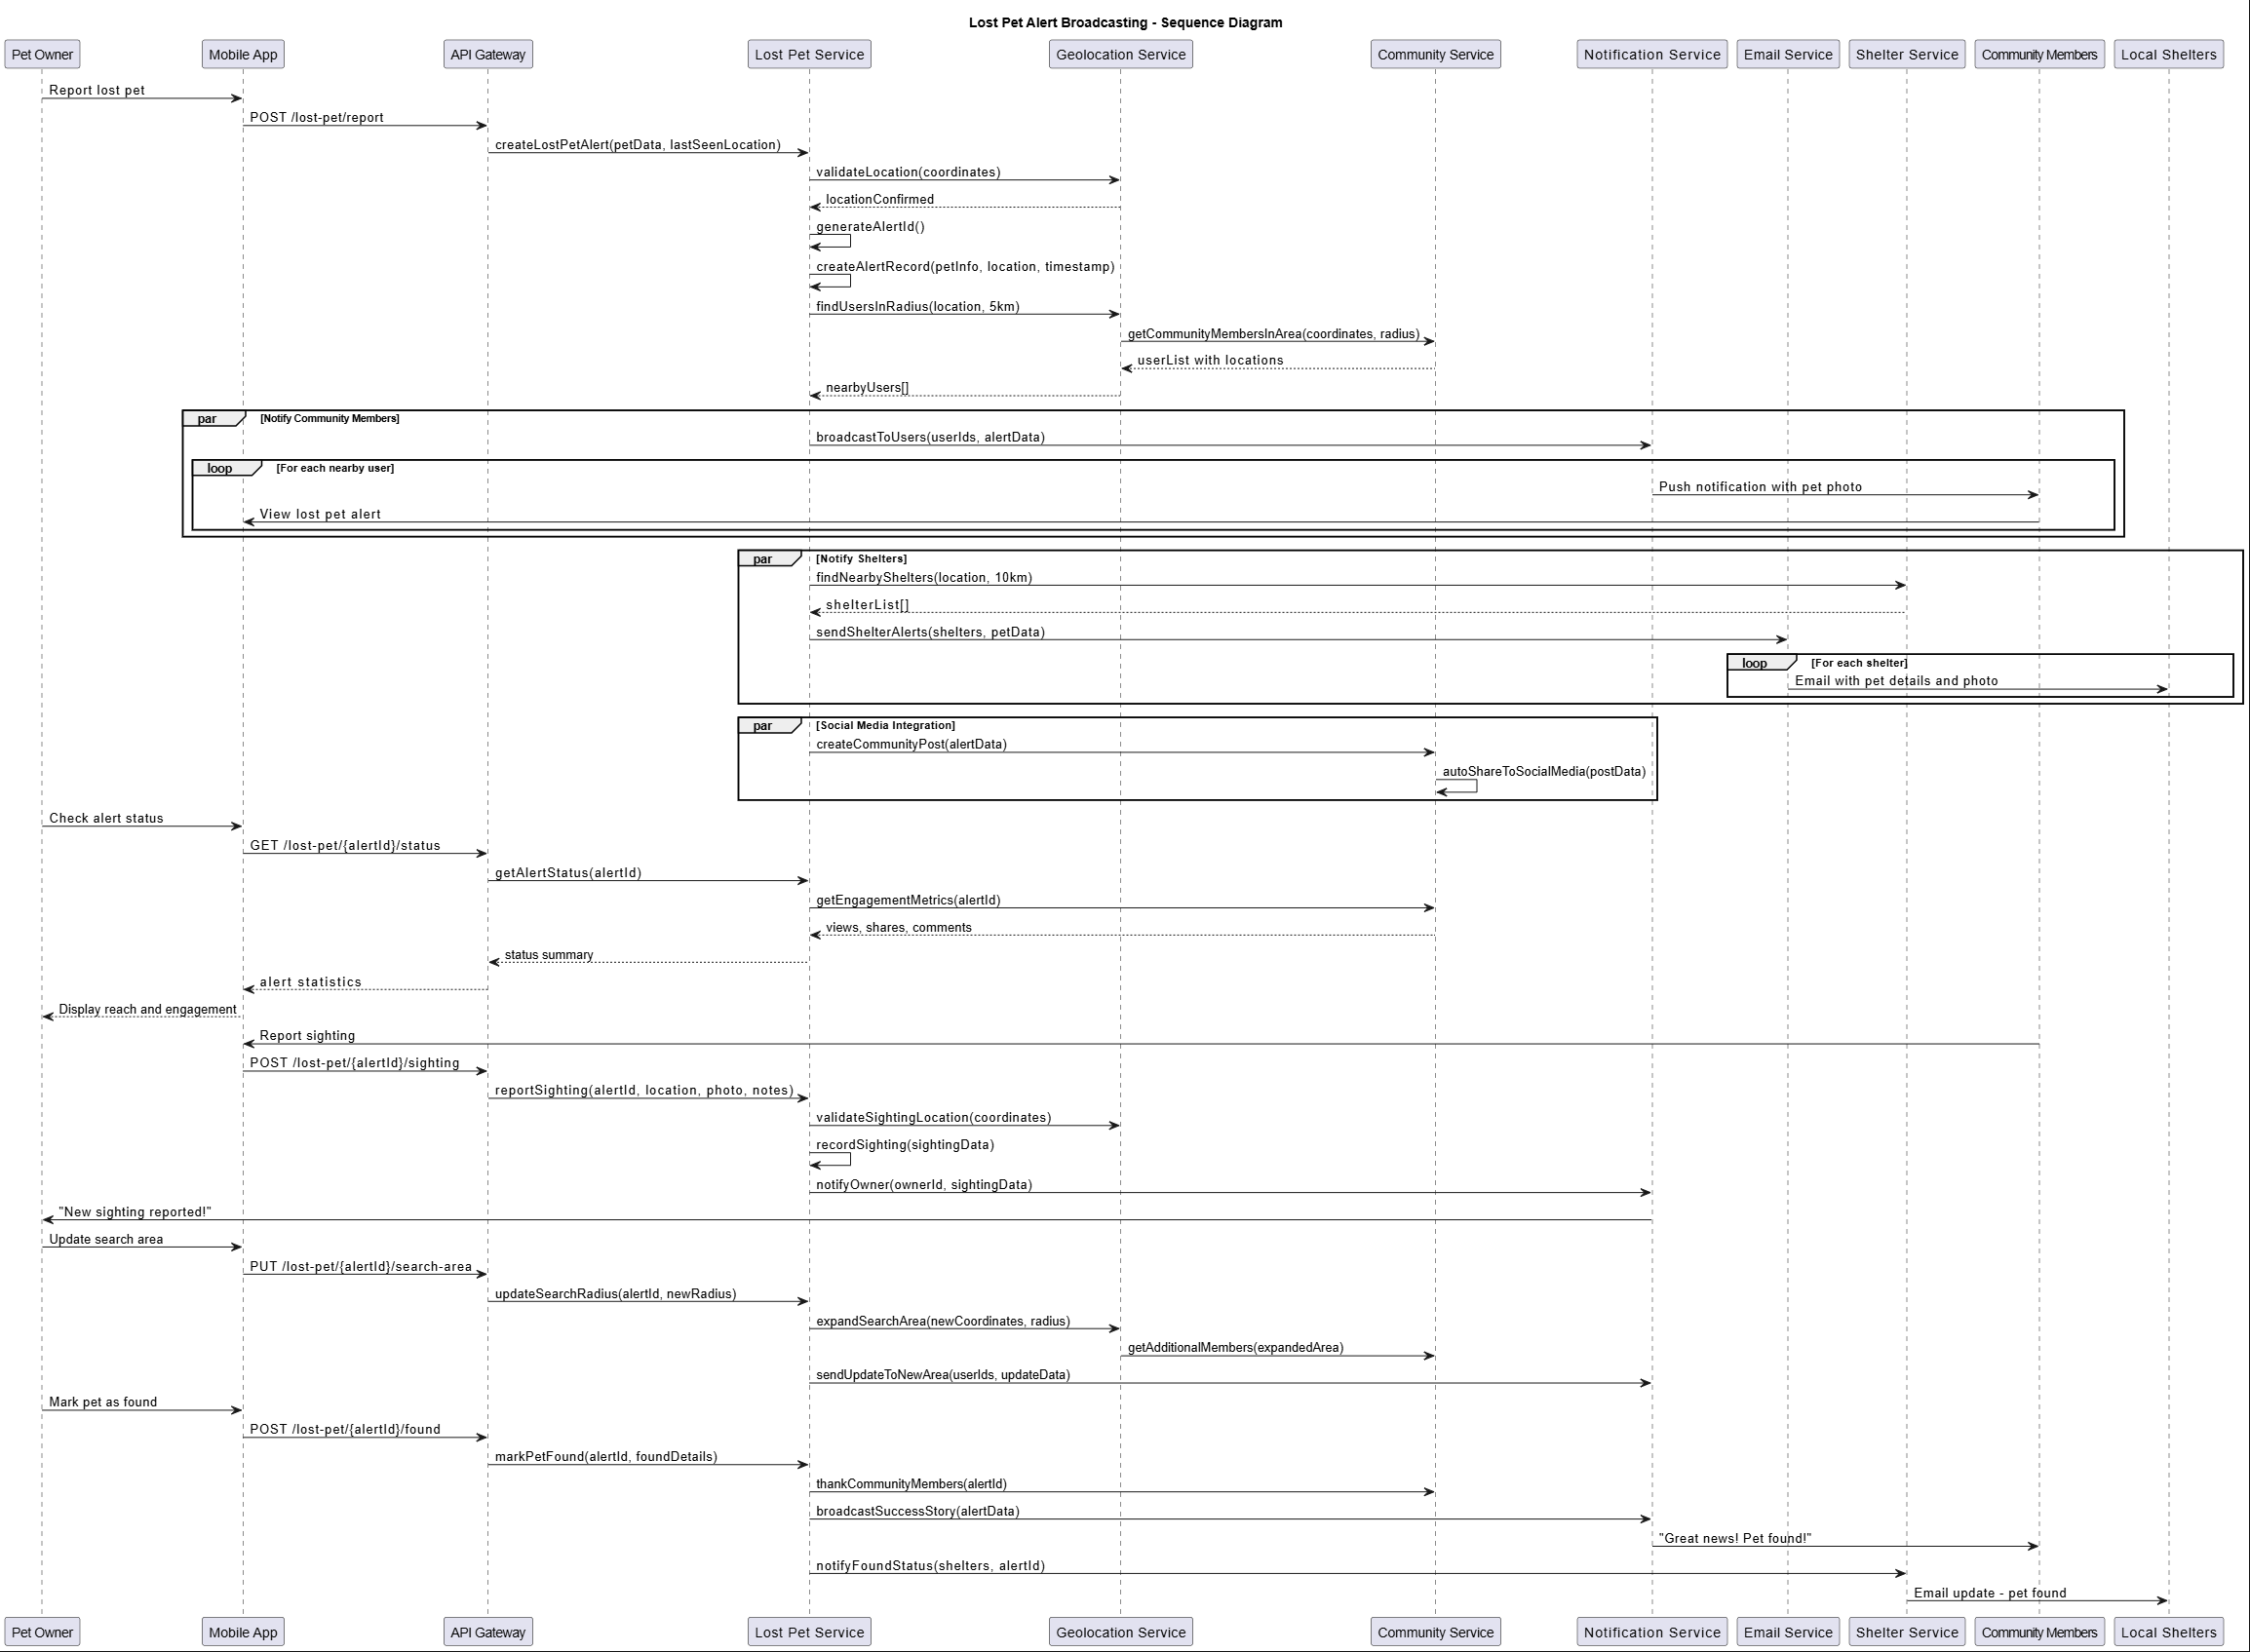
\includegraphics[width=1.0\textwidth]{ThesisFigs/sequence_lost_pet_alert_broadcasting.png}
    \caption{Lost Pet Alert Broadcasting Sequence Diagram}
    \label{fig:sequence_lost_pet_alert_broadcasting}
\end{figure}

This sequence diagram models the comprehensive lost pet alert broadcasting system, including GPS-based community member identification within a 5km radius, parallel notification delivery via push notifications and email, shelter coordination within a 10km radius, social media integration, real-time sighting reporting, and success story sharing upon pet recovery.

\subsubsection{Cryptocurrency Payment Processing}

\begin{figure}[H]
    \centering
    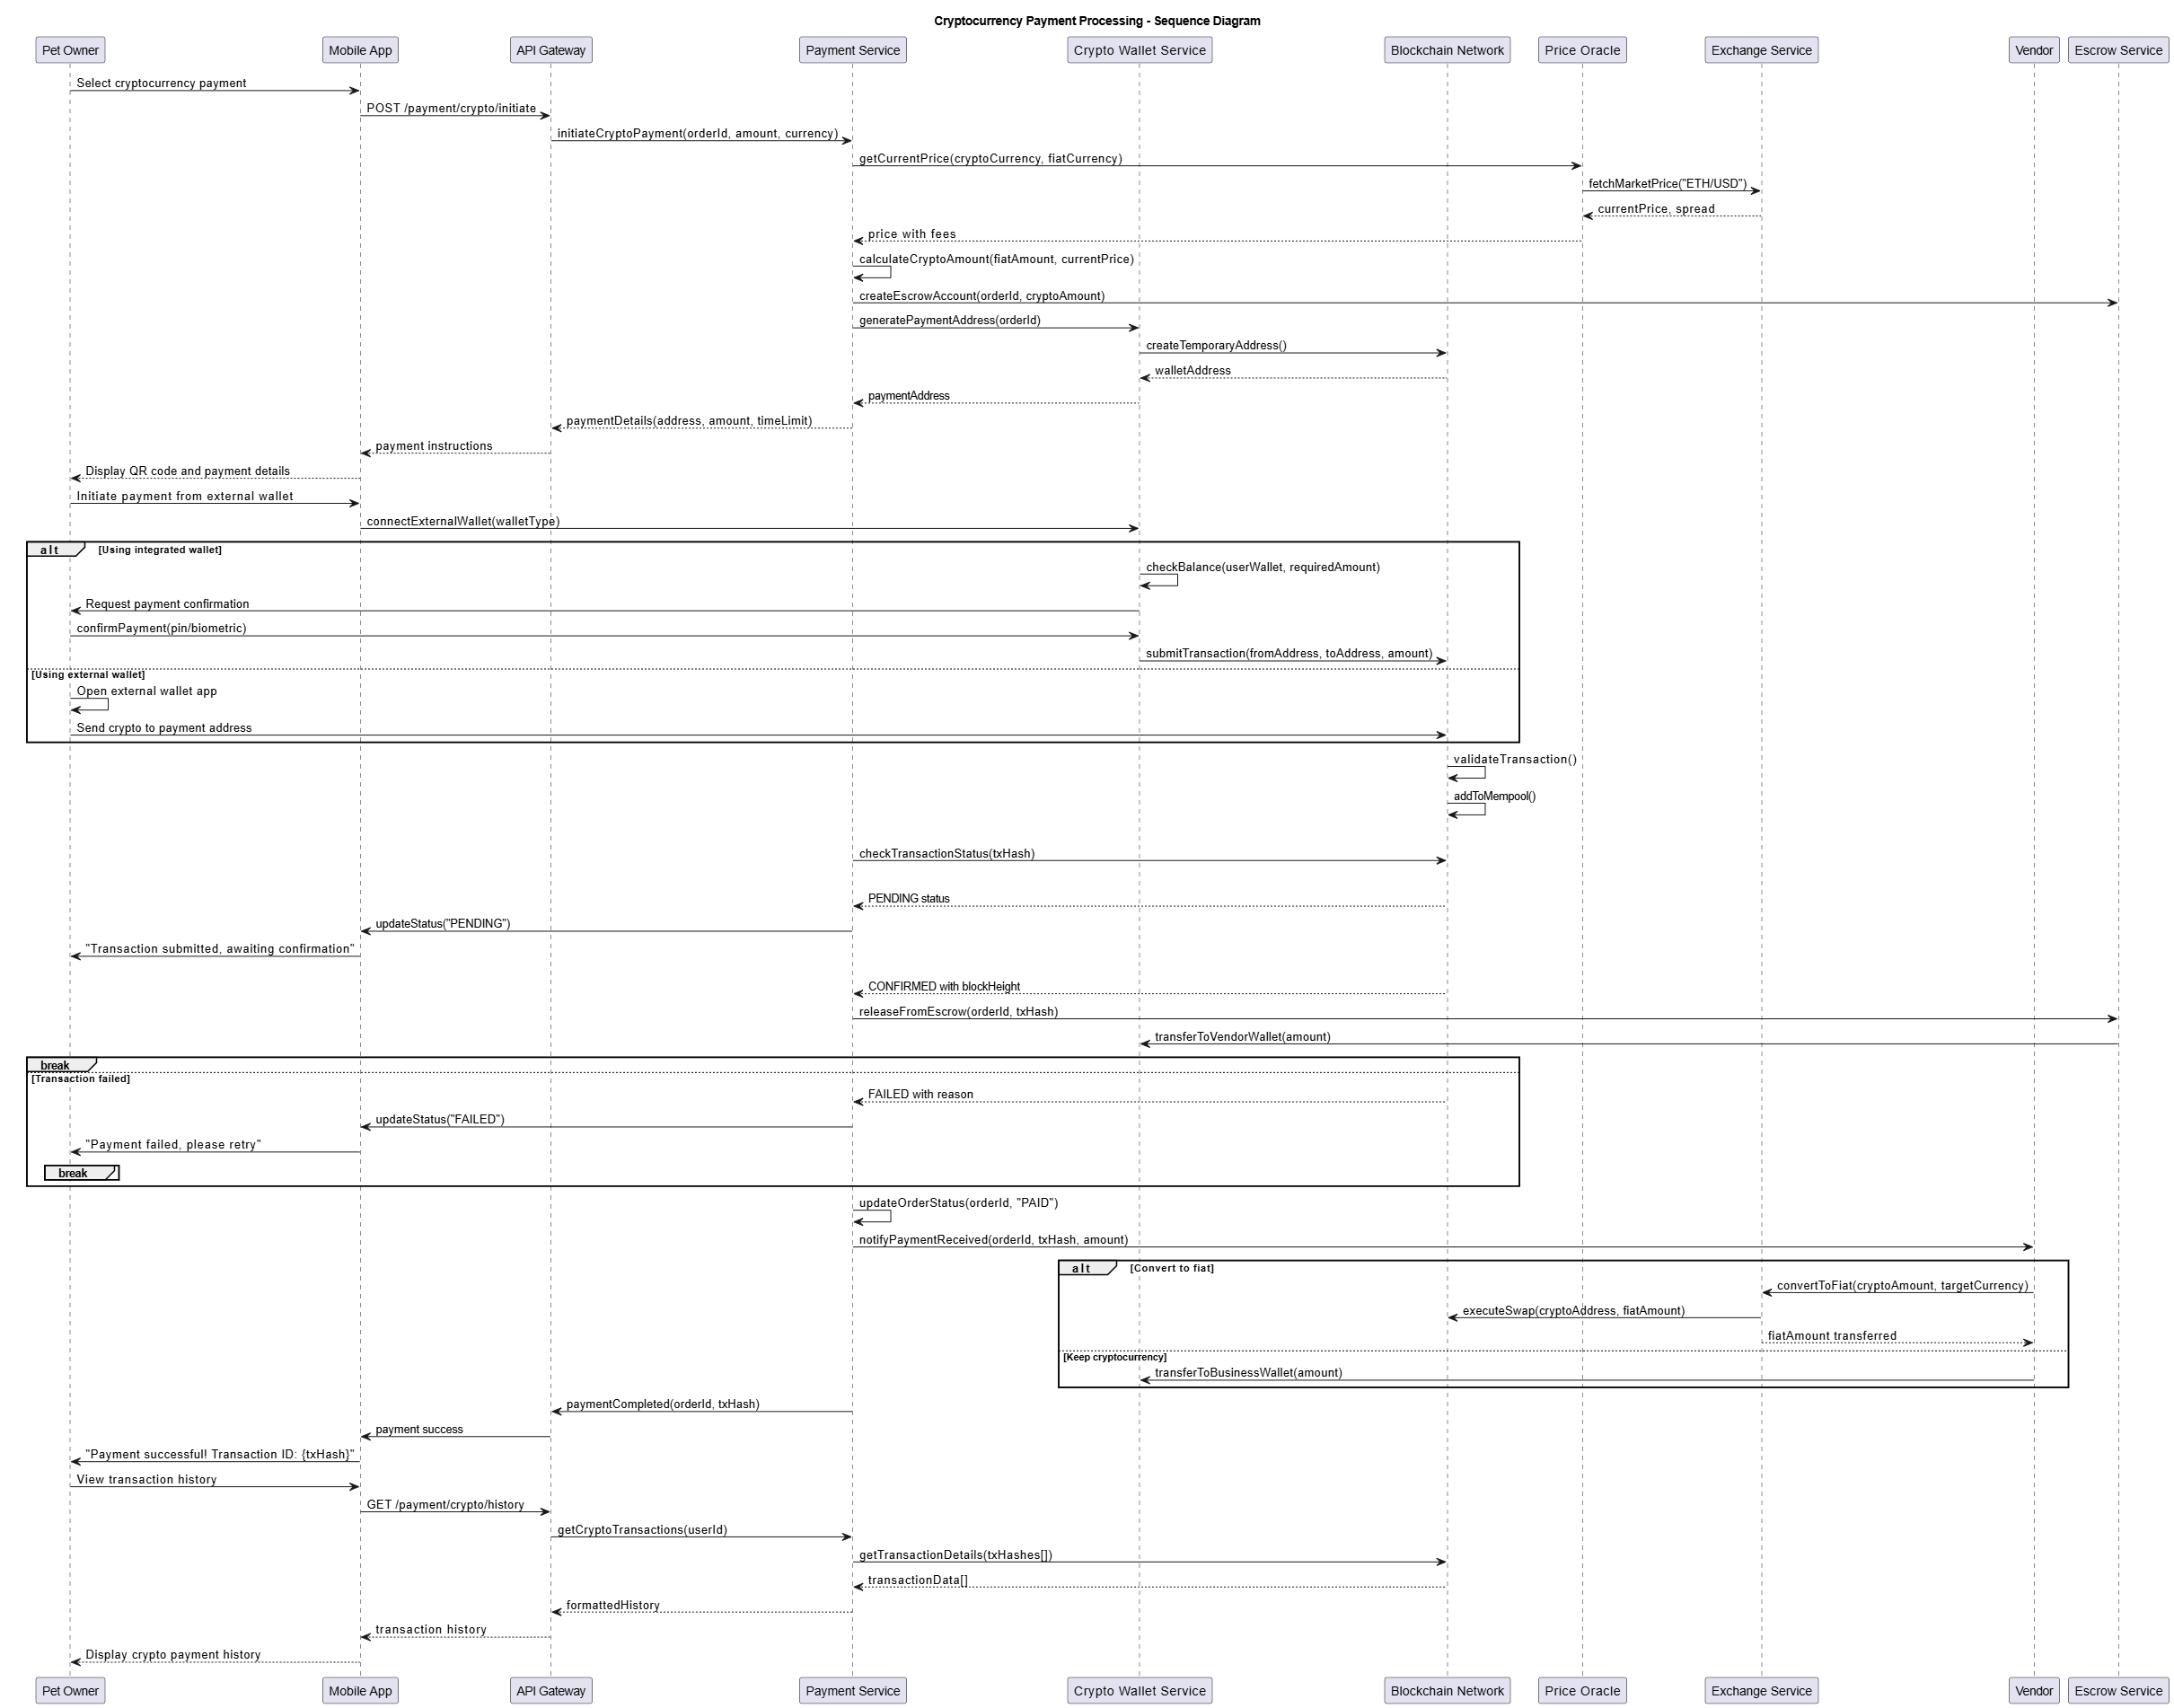
\includegraphics[width=1.0\textwidth]{ThesisFigs/sequence_cryptocurrency_payment_flow.png}
    \caption{Cryptocurrency Payment Flow Sequence Diagram}
    \label{fig:sequence_cryptocurrency_payment_flow}
\end{figure}

This advanced sequence diagram illustrates the cryptocurrency payment processing system including real-time price oracle integration, blockchain transaction monitoring, escrow service management, transaction confirmation tracking, and automated conversion options for vendors. The flow handles both integrated wallet payments and external wallet transactions with comprehensive error handling.

\subsection{State Transition Diagrams}

\subsubsection{Appointment Lifecycle}

\begin{figure}[H]
    \centering
    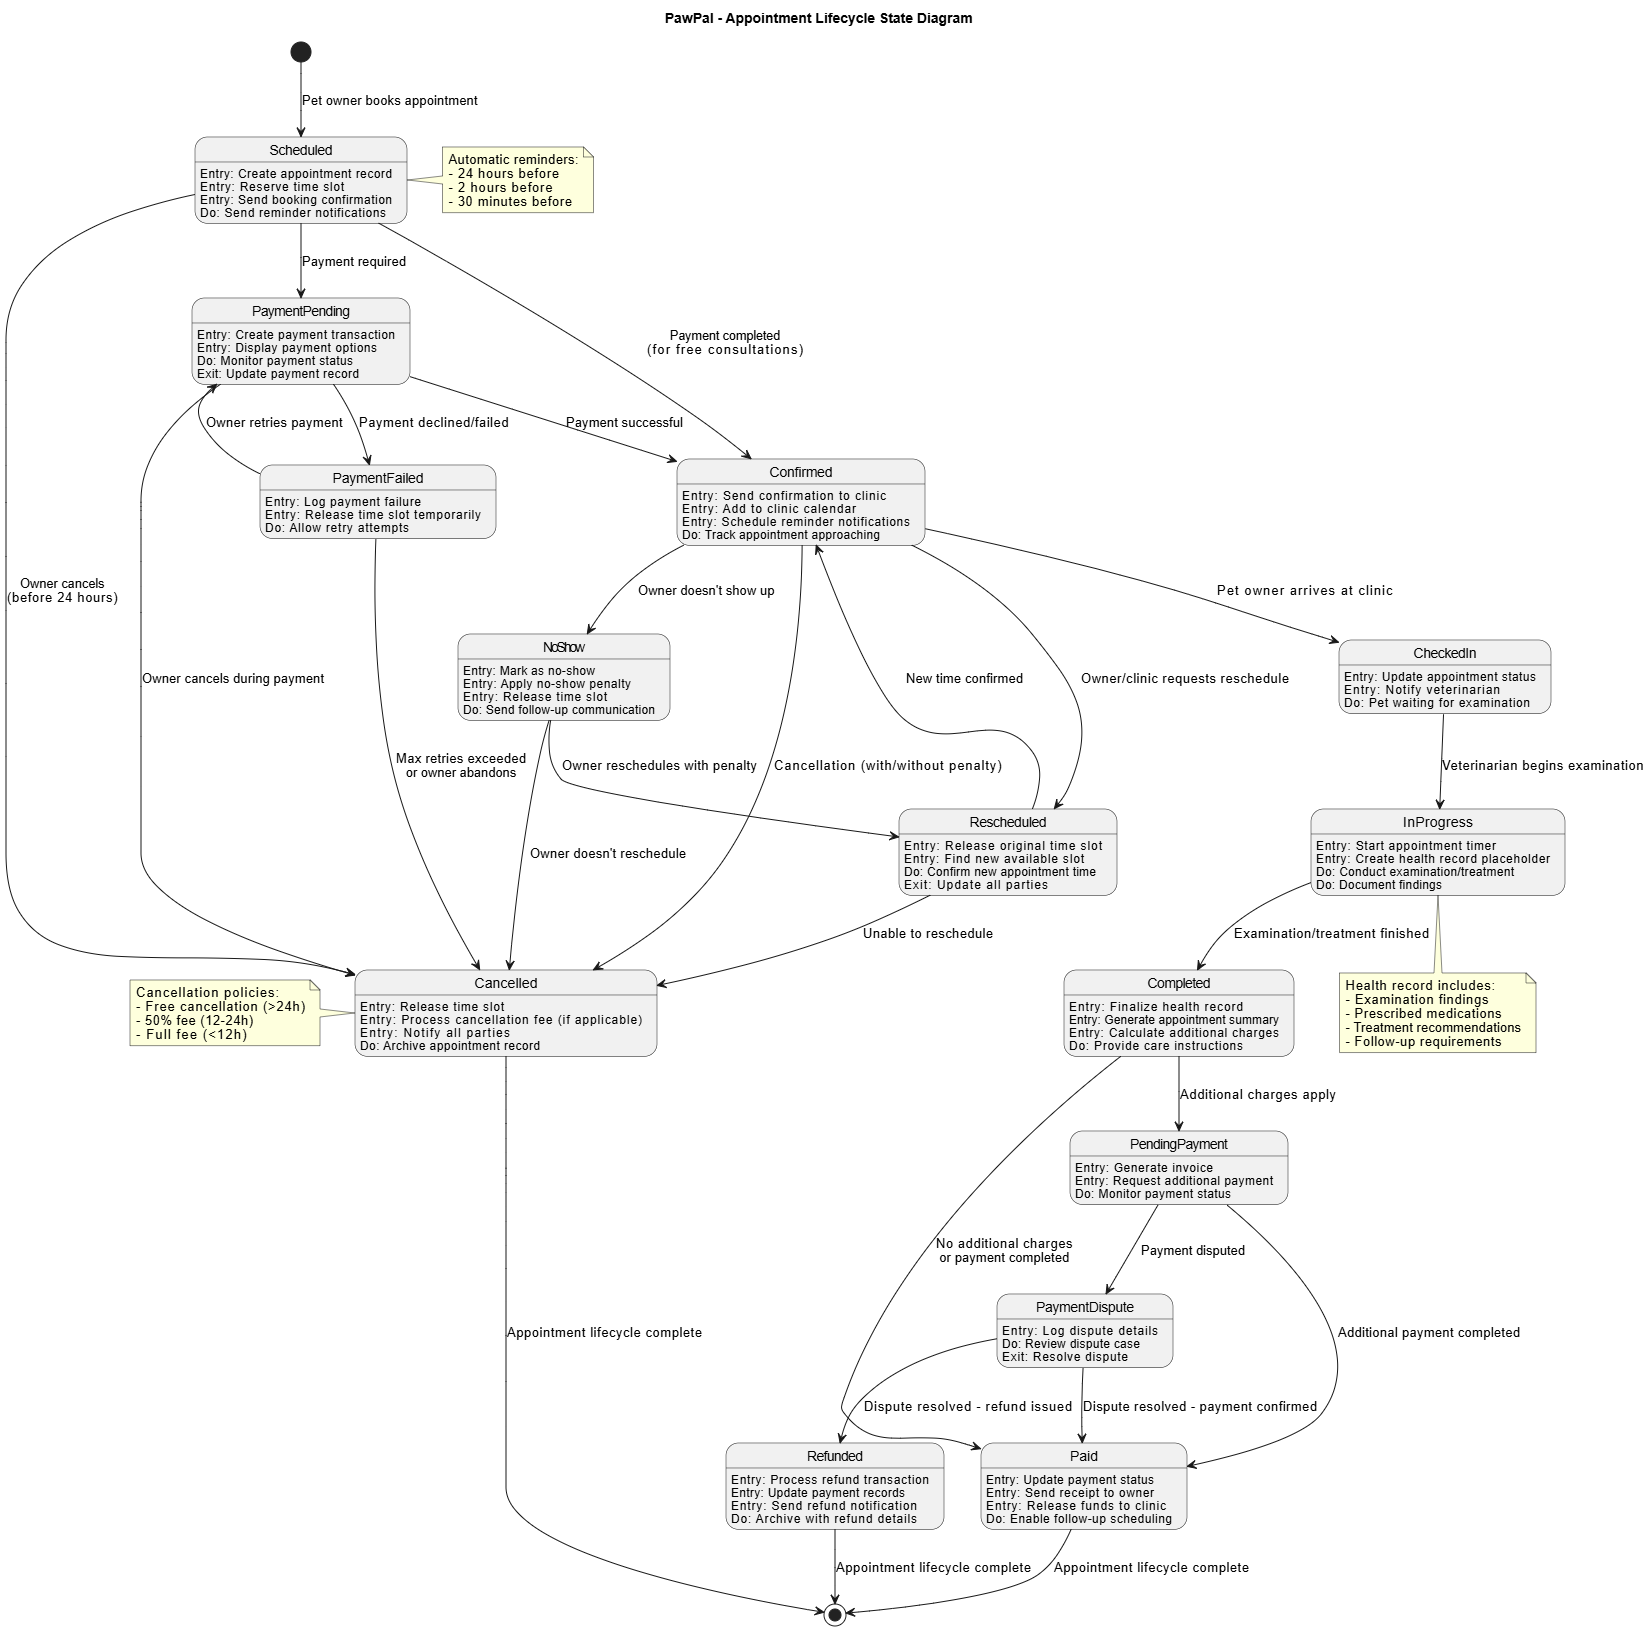
\includegraphics[width=1.0\textwidth]{ThesisFigs/state_appointment_lifecycle.png}
    \caption{Appointment Lifecycle State Diagram}
    \label{fig:state_appointment_lifecycle}
\end{figure}

This state diagram models the complete lifecycle of veterinary appointments from initial scheduling through completion, including payment processing, rescheduling options, cancellation policies, and no-show handling with appropriate state transitions and actions.


\subsubsection{Payment Transaction States}

\begin{figure}[H]
    \centering
    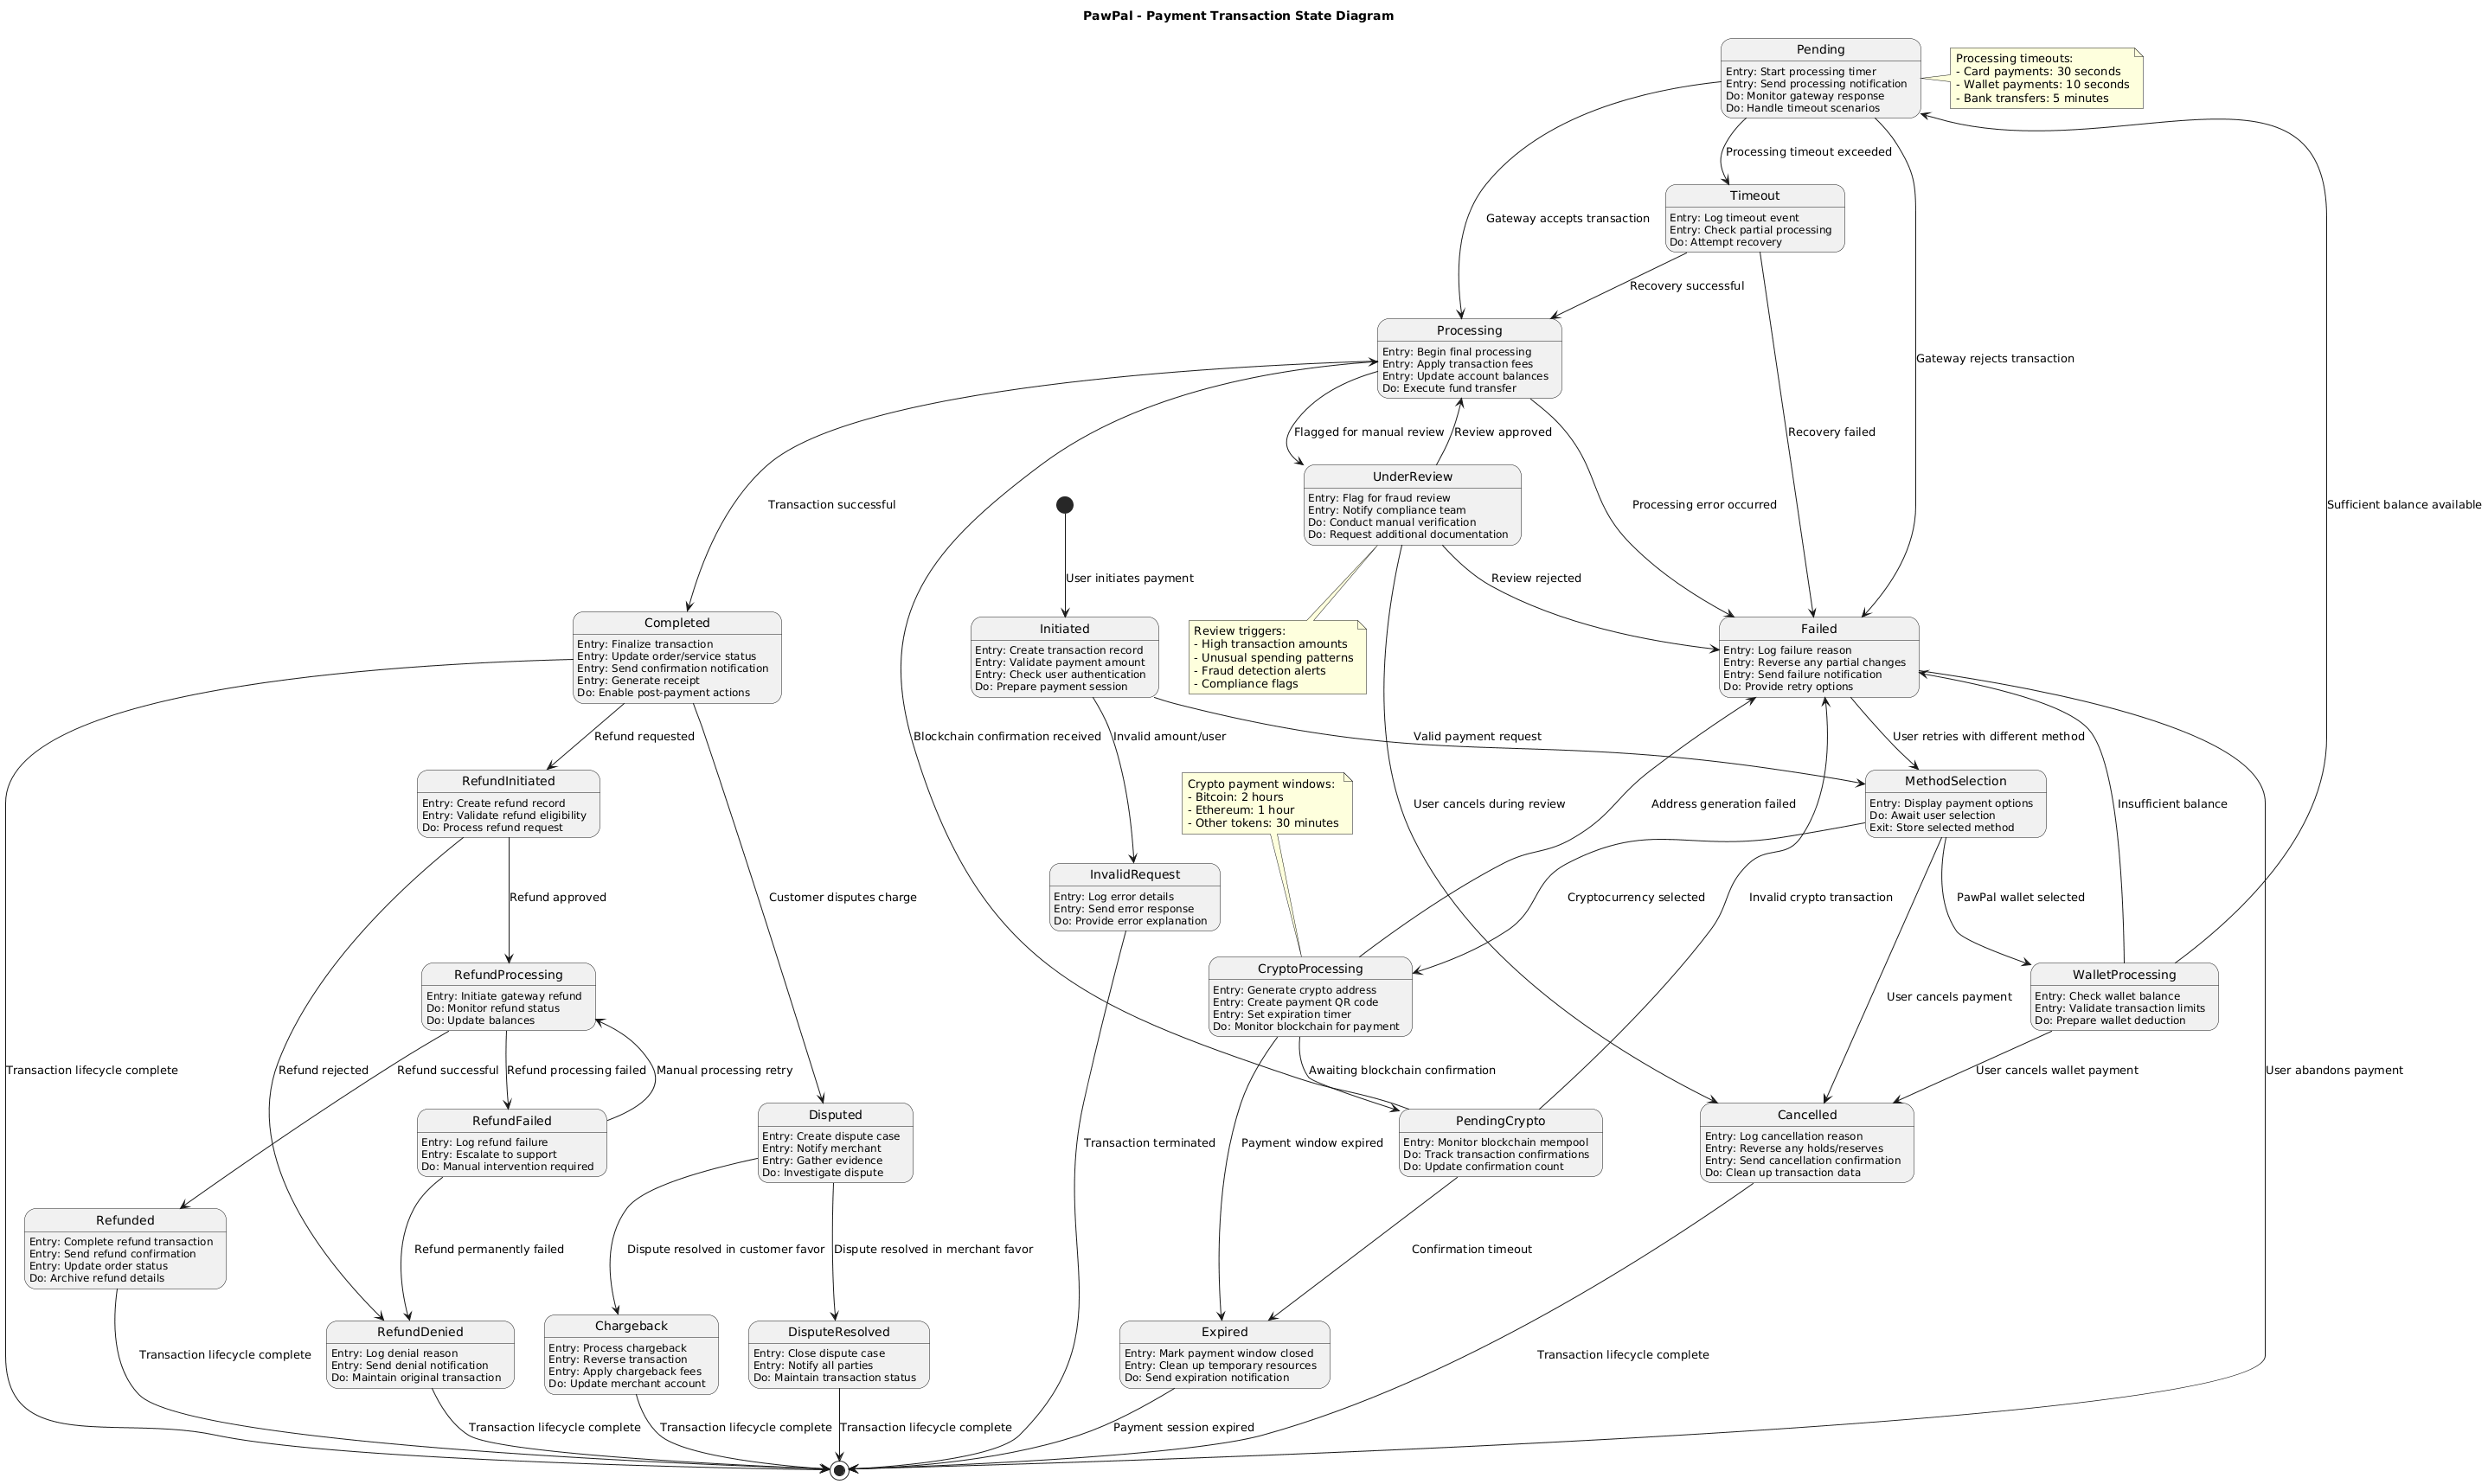
\includegraphics[width=1.0\textwidth]{ThesisFigs/state_payment_transaction.png}
    \caption{Payment Transaction State Diagram}
    \label{fig:state_payment_transaction}
\end{figure}

This state diagram illustrates the payment transaction lifecycle supporting multiple payment methods (card, wallet, cryptocurrency) with proper handling of processing states, timeout scenarios, fraud review processes, dispute resolution, and refund processing.

\subsubsection{Service Booking States}

\begin{figure}[H]
    \centering
    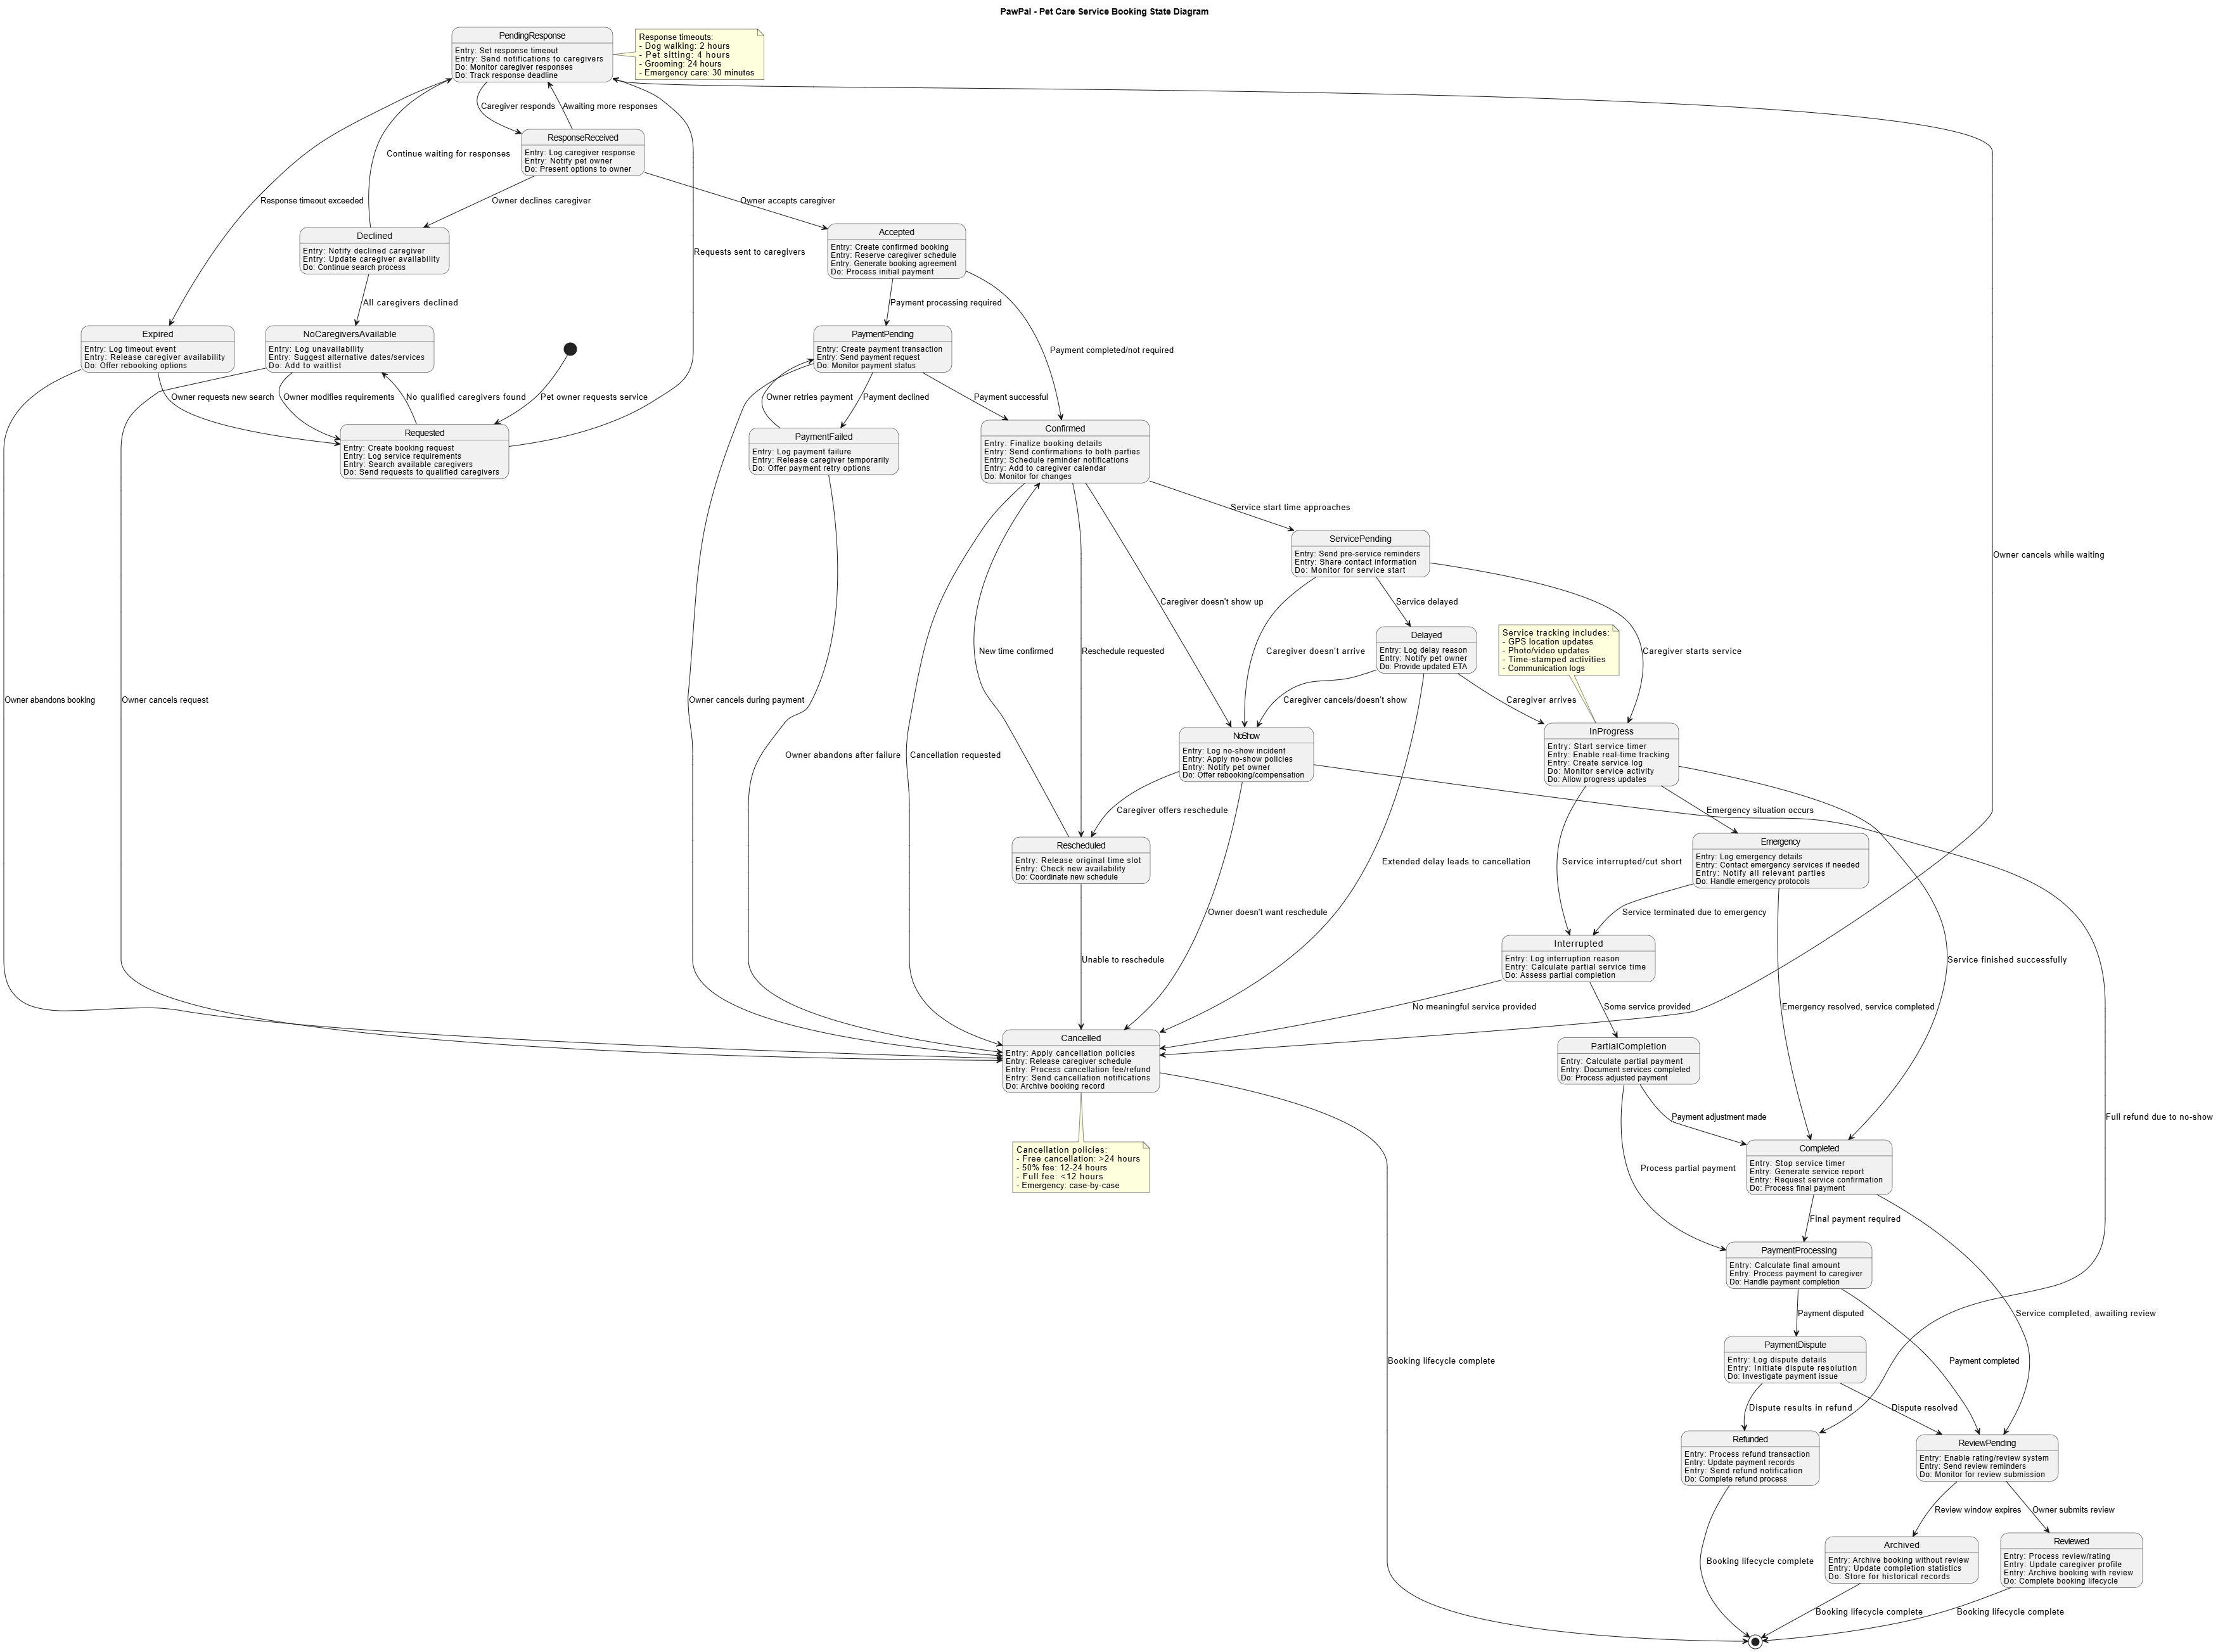
\includegraphics[width=1.0\textwidth]{ThesisFigs/state_service_booking.png}
    \caption{Service Booking State Diagram}
    \label{fig:state_service_booking}
\end{figure}

This state diagram models the pet care service booking lifecycle from initial request through service completion, including caregiver matching, booking confirmation, real-time service tracking, completion reporting, and review submission with comprehensive status management.

\subsubsection{Caregiver Service Lifecycle}

\begin{figure}[H]
    \centering
    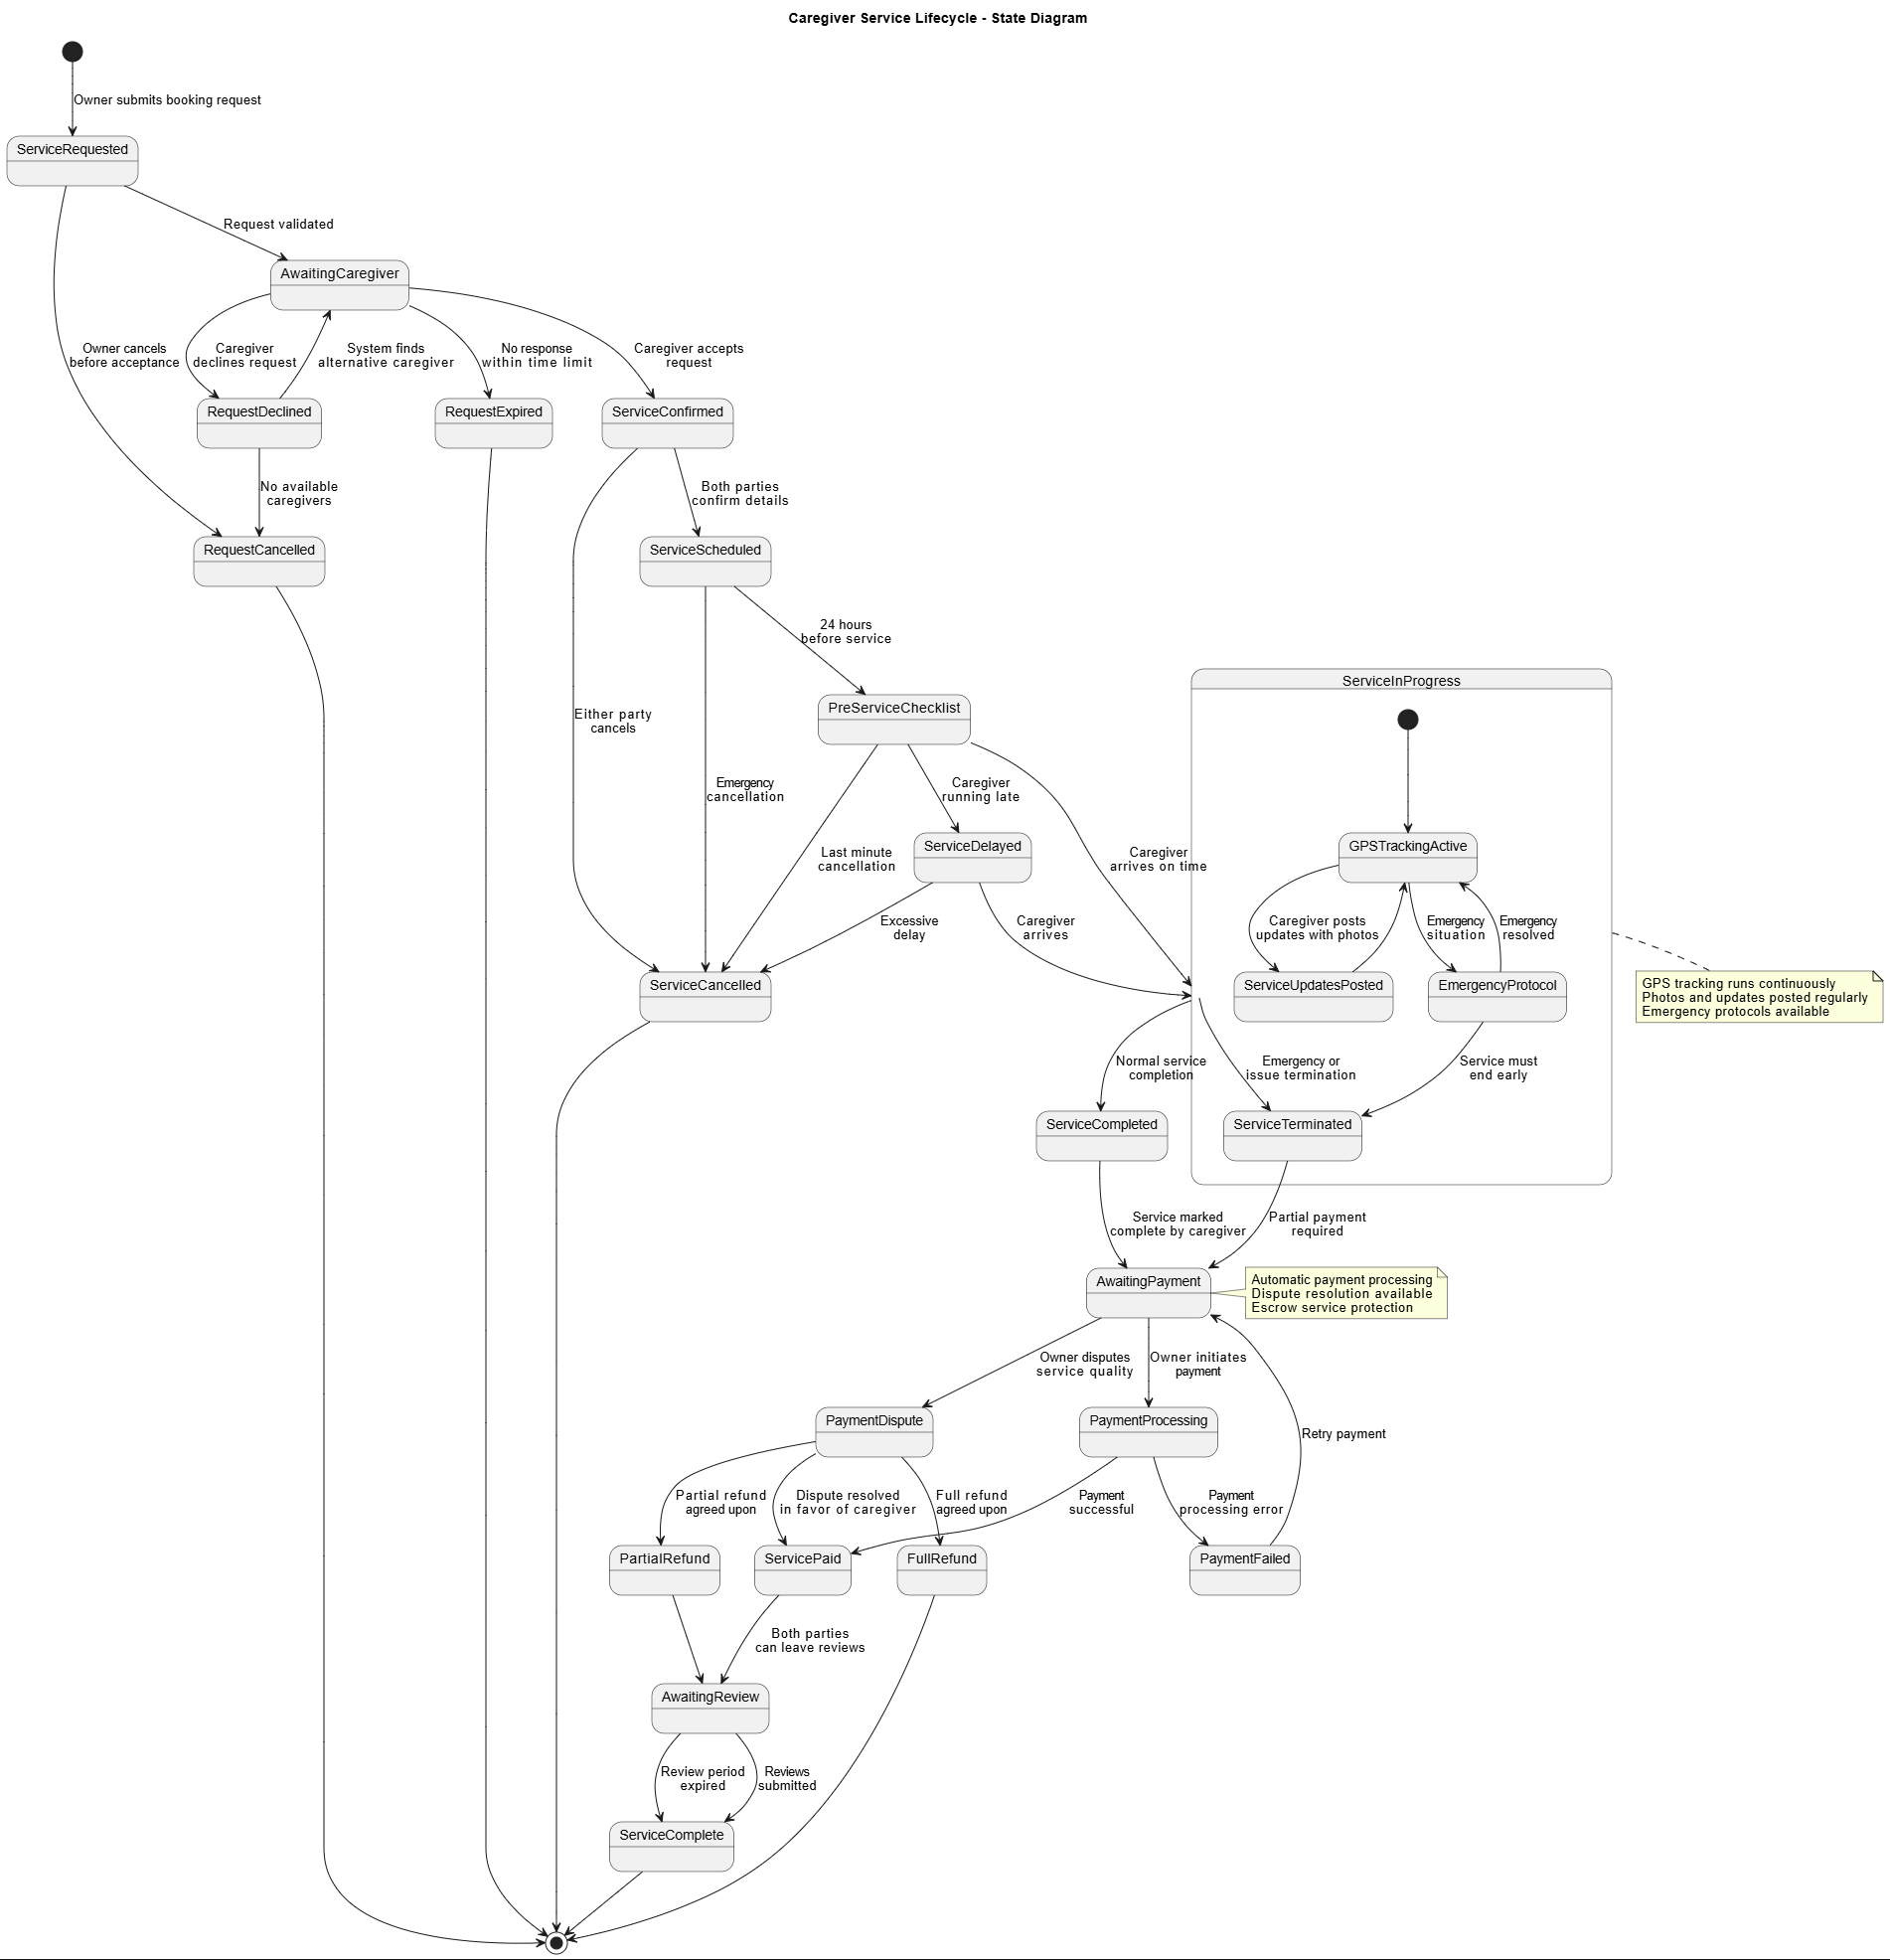
\includegraphics[width=1.0\textwidth]{ThesisFigs/state_caregiver_service_states.png}
    \caption{Caregiver Service Lifecycle State Diagram}
    \label{fig:state_caregiver_service_states}
\end{figure}

This comprehensive state diagram models the complete caregiver service lifecycle from initial booking request through service completion and review. The diagram includes detailed states for service confirmation, GPS tracking activation, emergency protocols, payment processing, dispute resolution, and review collection with proper state transitions and timeout handling.

\subsubsection{Lost Pet Alert Lifecycle}

\begin{figure}[H]
    \centering
    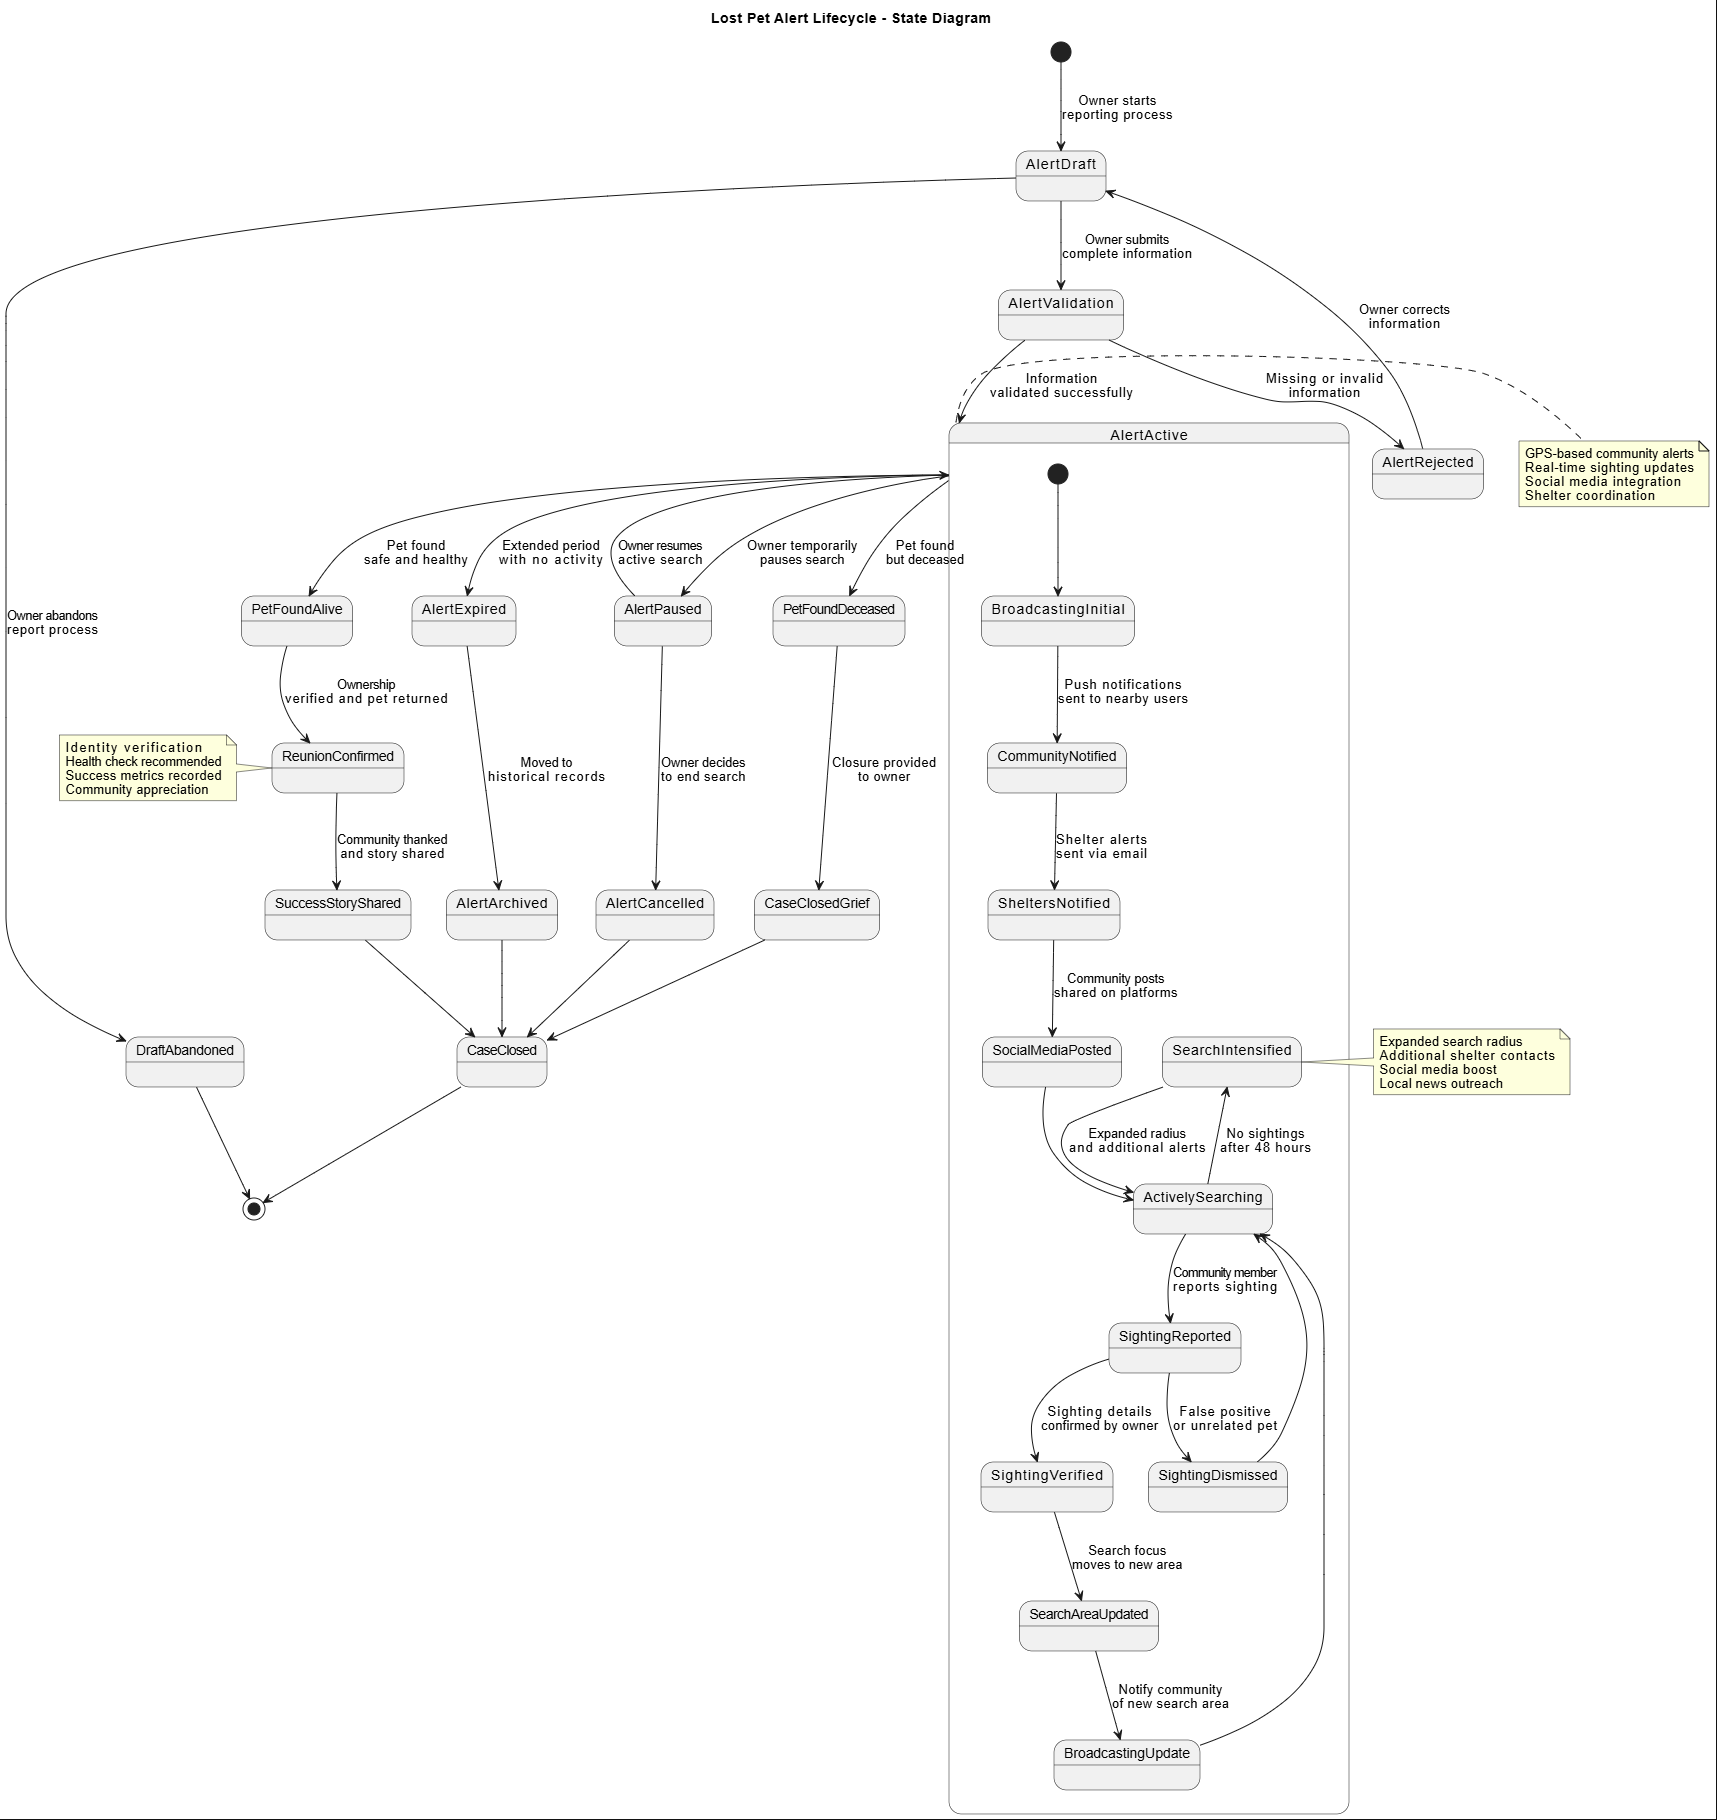
\includegraphics[width=1.0\textwidth]{ThesisFigs/state_lost_pet_alert_states.png}
    \caption{Lost Pet Alert Lifecycle State Diagram}
    \label{fig:state_lost_pet_alert_states}
\end{figure}

This state diagram tracks the lost pet alert lifecycle including alert validation, community broadcasting phases, sighting verification, search area updates, and resolution tracking. The diagram handles both successful reunions and closure scenarios with appropriate community notifications and case archival processes.

\subsubsection{User Account Management}

\begin{figure}[H]
    \centering
    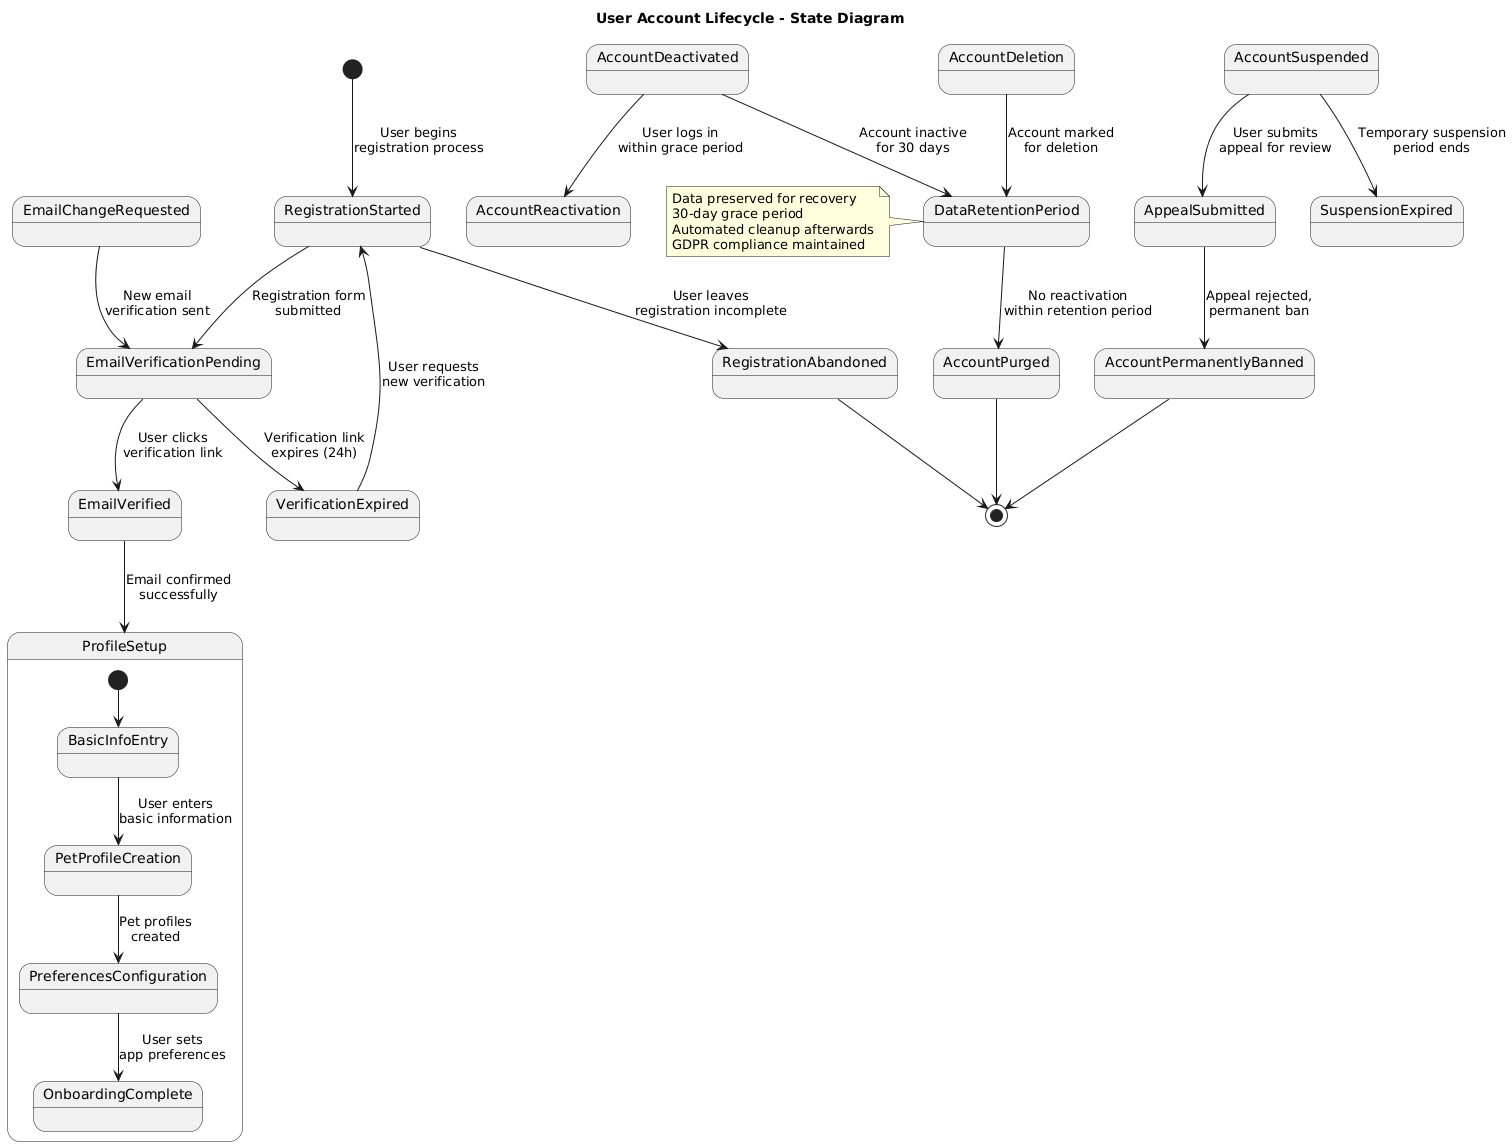
\includegraphics[width=1.0\textwidth]{ThesisFigs/state_user_account_states.png}
    \caption{User Account Lifecycle State Diagram}
    \label{fig:state_user_account_states}
\end{figure}

This comprehensive state diagram models the complete user account lifecycle from registration through account termination. The diagram includes email verification, profile setup phases, account status management (active, restricted, suspended), premium subscription handling, deactivation and reactivation processes, data retention policies, and GDPR compliance procedures.

\clearpage

